% !TEX root = catron-dissertation.tex
% arara: pdflatex
% arara: bibtex
% arara: pdflatex
% arara: pdflatex

\documentclass[twoadvisors,noinfo,final]{nddiss2e}

\usepackage{graphicx}
\usepackage{subcaption}
\usepackage{epstopdf}
\epstopdfsetup{outdir=./images/}
\usepackage{listings}
\usepackage{amsmath,amssymb}
% \usepackage[makeroom]{cancel}
% \usepackage{csquotes}
% \usepackage{fdsymbol}
% \usepackage{physics}
% \usepackage{mathtools}
\usepackage[export]{adjustbox}
\usepackage{multirow}
\usepackage{longtable,tabularx}
\usepackage{xcolor}
\usepackage{tikz}
\newcommand*\circled[1]{\tikz[baseline=(char.base)]{
    \node[shape=circle,draw,inner sep=2pt] (char) {#1};}}
\newcommand*\circledfill[1]{\tikz[baseline=(char.base)]{
    \node[shape=circle,draw,inner sep=2pt,fill=white] (char) {#1};}}
\newcommand*\squared[1]{\tikz[baseline=(char.base)]{
    \node[shape=rectangle,draw,inner sep=2pt] (char) {#1};}}

\lstset
{ %Formatting for code in appendix
    language=Matlab,
    basicstyle=\footnotesize,
    numbers=left,
    stepnumber=1,
    showstringspaces=false,
    tabsize=1,
    breaklines=true,
    breakatwhitespace=false,
}

% Custom Math Objects
\DeclareMathOperator{\fft}{FFT}
\DeclareMathOperator{\fftn}{FFT_n}
\DeclareMathOperator{\fftthree}{FFT_3}
\DeclareMathOperator{\ffttwo}{FFT_2}
\DeclareMathOperator{\fftshift}{FFT_{SHIFT}}
\DeclareMathOperator{\ifft}{IFFT}
\DeclareMathOperator{\ifftn}{IFFT_n}
\DeclareMathOperator{\wf}{WF}
\DeclareMathOperator{\f}{F}
\DeclareMathOperator{\opd}{OPD}
\DeclareMathOperator{\opdrms}{OPD_{RMS}}
\DeclareMathOperator{\opl}{OPL}
\DeclareMathOperator{\sr}{SR}
\DeclareMathOperator{\spl}{SPL}
\DeclareMathOperator{\real}{REAL}
\DeclareMathOperator{\imag}{IMAG}
\DeclareMathOperator{\ft}{FT}


\begin{document}
  \frontmatter
    \title{ Filtering of Acoustic Information from Aero-Optical Measurements }
    \author{ Brian Lowell Catron }
    \work{ Dissertation }
    \degaward{ Doctor of Philosophy }
    \advisor{ R. Mark Rennie }
    \secondadvisor{ Eric J. Jumper}
    \department{ Aerospace and Mechanical Engineering}

    \maketitle
    \copyrightyear{ 2022 }
    \makecopyright

    \begin{abstract}
      % !TEX root = catron-dissertation.tex

With development of new airborne optical systems, there is a significant amount of effort being put into maximizing the farfield performance of these optical systems.
To meet this goal, the root mean square of the optical path difference, $\opdrms$, over the aperture, a measure of the nearfield optical distortions, is being reduced as much as possible.
Part of this development process involves testing models of these systems with various configurations in wind tunnels.
In these tests, the optical disturbances due to the testing environment are becoming a large percentage of the measured optical disturbances.
It is now a necessity to be able to identify, measure, and remove the various noise sources that appear in aero-optical measurements that take place in wind tunnels.

One of the primary sources of signal noise in these measurements, is acoustics.
Both the wing-tunnel fan and the flow through out the tunnel generate large amounts of acoustic noise that travel throughout the tunnel as acoustic duct modes.
The fan generates strong narrow-band signals at the blade-passing frequency and its harmonics.
There are also significant broad-band acoustic duct mode signals along with vibration related signals and strong mostly-steady optical lensing signals that add to the overall measurement.

A significant portion of this dissertation is dedicated to analyzing wind-tunnel optical wavefront data in multidimensional spectral space.
The signal identification and filtering mostly take place in the multidimensional spectrum, where the optical wavefront is not only split into its temporal frequency components but also its spatial frequency components.
A combination of three filters is able to remove most of the noise signals while retaining most of the aero-optical signal.
A velocity filter, which retains a narrow band of signal that is traveling within a small velocity range, is able to remove most of the broad-band signal noise, especially at higher temporal-frequencies.
A backward filter, which retains only the portion of a signal that is traveling in the direction of flow, removes signal that the velocity filter is not able to at lower temporal-frequencies.
Finally a baseline filter identifies the baseline spectrum and removes narrow-band peaks.

    \end{abstract}
    \begin{dedication}
      To my wife Karen \& our son Arthur
    \end{dedication}

    \tableofcontents
    \listoffigures
    \listoftables
    \begin{symbols}[cl]
% A
\sym{Ap}{Aperture size - Typically diameter}
% B
% C
% D
% E
% F
% G
% H
% I
\sym{I}{Actual on target intensity}
\sym{I_0}{Diffraction-limited intensity}
% J
% K
\sym{k}{Wavenumber ($k=2\pi/\lambda$)}
% L
% M
% N
\sym{n}{Index of refraction}
% O
\sym{\opd}{Optical path difference}
\sym{\opdrms}{Time-averaged spatial $\opd$ root-mean-square}
\sym{\opdrms(t)}{Spatial $\opd$ root-mean-square as a function of time}
% P
% Q
% R
% S
\sym{\sr}{Strehl ratio ($\textrm{SR}=I/I_0$)}
% T
% U
% V
% W
% X
% Y
% Z
\sym{}{\textbf{Greek}}
% ALPHA
% BETA
% GAMMA
% DELTA
\sym{\delta}{Boundary layer thickness}
% EPSILON
% ZETA
% ETA
% THETA
\sym{\left<\theta^2\right>}{Mean-squared of the fluctuating deflection angle}
% IOTA
% KAPPA
% LAMBDA
% MU
% NU
% XI
% OMICRON
% PI
% RHO
% SIGMA
% TAU
% UPSILON
% PHI
% CHI
% PSI
% OMEGA
\end{symbols}


    \begin{acknowledge}
      I would like to thank my advisors R. Mark Rennie and Eric J. Jumper along with Stanislav Gordeyev for helping me grow not only in my ability to take measurements, but also as a researcher, designing experiments and analyzing the data.
I would also like to think my fellow grad students, particularly Jon Wells, Barry Pawlowski, Matt Kalensky, and Matt Kemnetz, who endured alongside me.
You helped me when I needed help and gave me some interesting problems to solve.

Most of all I would like to thank my family.
My parents, Kevin and Nila, who pushed me to meet my potential when I was younger.
I would like to think you for the sacrifices you made for my benefit.
Thank you Karen, my wife, for putting up with my slow progress at times.
Thank you for everything you do for me and our child.
Arthur, watching you grow and learn brings me joy everyday.
% Elizabeth, I will always miss you and will have an emptiness from never having the opportunity to hold you.

    \end{acknowledge}

  \mainmatter
    % !TEX root = catron-dissertation.tex
\epstopdfsetup{outdir=./images/01_introduction/}

\chapter{Introduction}
\label{chap:01_intro}

There have been two major attempts to field a directed-energy system aboard an aircraft to date \cite{Jumper-2013-8KtN3pue}.
The first was the Airborne Laser Laboratory (ALL) which took place in the late 1970's and early 1980's which used a CO$_2$ laser with a wavelength of 10.6-$\mu$m.
The second was the Airborne Laser (ABL) program which operated in the 2000's and used a COIL laser at 1.315-$\mu$m.
Airborne optical systems like ALL and ABL have to deal with a phenomenon known as ``aero-optics,'' which refers to optical distortions caused by compressible aero-dynamic flow features that pass through the outgoing beam.
These optical distortions were first noticed due to image degradation in wind tunnel measurements in the 1950's \cite{Stine-1956-UaRzVZCe} as well as in photo-reconnaissance missions in the 1960's \cite{Kyrazis-2013-vwKeEBym}.

The peak on-target irradiance of a beam passing through an optical disturbance, $I$, divided by the diffraction-limited performance, $I_0$, is known as the Strehl ratio \cite{Mahajan-1982-kkXM4eaB}, $\sr$,
\begin{equation}
  \sr = \frac{I}{I_0} \textrm{.}
  \label{eqn:01_strehl_ratio_definition}
\end{equation}
The diffraction-limited performance is the beam intensity that would exist on the same target if not for the optical disturbance.
The Airborne Laser Laboratory had an estimated Strehl ratio of 95\%\cite{Jumper-2013-8KtN3pue} so that the ``aero-optics problem'' effectively did not apply for this case.
Following the Airborne Laser Laboratory program there was a desire to move toward shorter wavelengths in order to take advantage of improved diffraction-limited performance, leading to a smaller-diameter focused spot on target with a higher irradiance $I_0$: \cite{Jumper-2001-6QDh7zDy},
\begin{equation}
  \frac{I_0}{P} = \frac{1}{\pi}\left(\frac{Ap}{\lambda z}\right)^2 \textrm{,}
  \label{eqn:01_farfield_intensity}
\end{equation}
where $P$ is the laser output power, $Ap$ is the aperture size, and $z$ is the propagation distance.
The improvement in diffraction-limited performance as the laser wavelength is decreased is shown in Figure \ref{fig:01_farfield_intensity}.
\begin{figure}
  \centering
  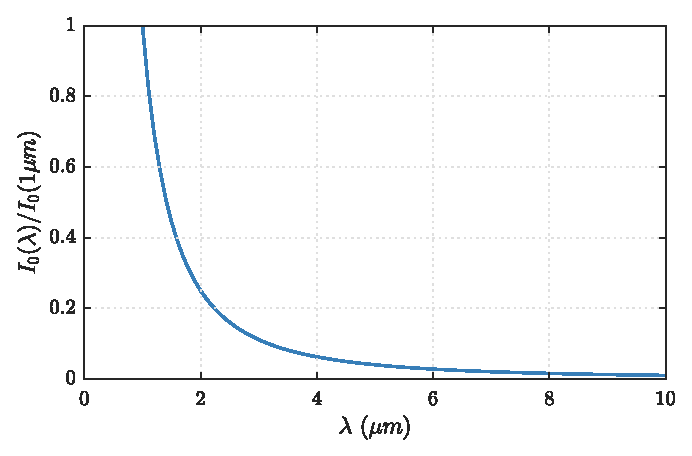
\includegraphics{../matlab/01_introduction/farfield_intensity.eps}
  \caption{Diffraction-limited far-field intensity of a beam normalized by the performance at 1-$\mu$m.}
  \label{fig:01_farfield_intensity}
\end{figure}
By only changing the laser source from a 10-$\mu$m to 1-$\mu$m wavelength the diffraction-limited performance can be increased 100 times.

Aero-optical issues start to become important as the wavelength is decreased as is evident from the Mar\'echal approximation \cite{Mahajan-1983-hg7ahvJM} which relates the Strehl ratio to wavelength,
\begin{equation}
  \sr \approx \exp\left\{-\left[\frac{2\pi \opdrms}{\lambda}\right]^2\right\} \textrm{,}
  \label{eqn:01_strehl_ratio}
\end{equation}
where $\opdrms$ is the spatial root-mean-square of the optical path difference over the aperture and is a way to quantify the optical disturbance as will be discussed further in Chapter \ref{chap:02_lit_review}.
As stated above, the ALL had a Strehl ratio of 95\%; however, if the ALL system's laser was swapped with another laser of a lower wavelength, the Strehl ratio would significantly decrease as shown by Figure \ref{fig:01_strehl_ratio}.
\begin{figure}
  \centering
  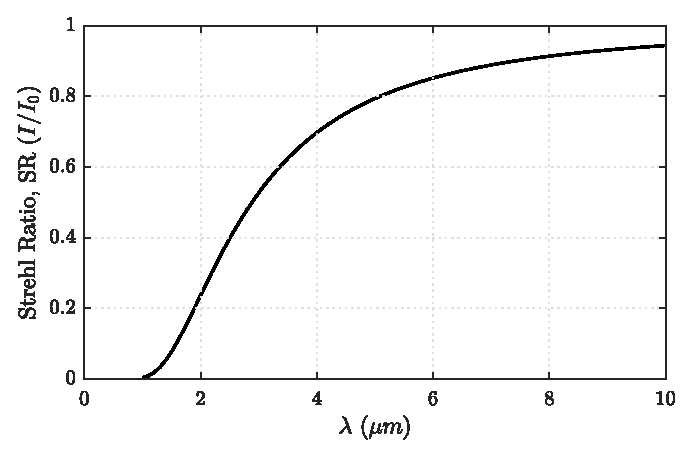
\includegraphics{../matlab/01_introduction/strehl_ratio.eps}
  \caption{Strehl ratio due to the $\opdrms$ of the Airborne Laser Laboratory (ALL) at various laser wavelengths.  ALL had an estimated Strehl ratio of 95\% with its 10.6-$\mu$m laser.}
  \label{fig:01_strehl_ratio}
\end{figure}
While going from 10 to 1-$\mu$m hypothetically results in a 100-fold increase in diffraction-limited performance, the actual on-target intensity that this hypothetical system obtains would be essentially zero due to the much larger effect that aero-optical aberrations have on the outgoing beam as the wavelength is reduced.
This means that the aero-optical problem can no longer be ignored, which was recognized as one of the main developmental risks of the ABL program \cite{DOTE-1999-HnkadUEw}.

As the next generation of airborne directed-energy systems are developed some amount of ground testing of those systems will need to occur.
In order to understand the aero-optical environment that these systems will experience in the air, wind tunnel tests will need to be employed.
These tests are cheaper to perform than, for example, flight testing, and allow for quicker iteration of design parameters.
However, as will be described in further detail in Chapter \ref{chap:02_lit_review}, wind-tunnel measurements of aero-optical effects typically require passing a test beam into and through the test-section, so that the test beam is susceptible to acquiring additional optical contamination including but not limited to the boundary layer present on the wall and the acoustic environment generated by the wind tunnel fan \cite{Gordeyev-2014-jcJndkHM}.
Note that it is common in signal-processing terminology to use the word “noise” to describe unwanted interference that appears in addition to the “signal” that is the objective of the measurement; however, in this dissertation, the word “contamination” is used to describe any optical noise sources that are unrelated to the aero-optical signal, in order to avoid confusion with use of the word “noise” to describe acoustic noise which, as will be shown, is also a source of optical contamination.

Assuming that the optical disturbances from aero-optical effects are statistically independent from the contaminating optical disturbances from the testing environment, we can estimate the total optical disturbance as
\begin{equation}
  \opdrms_{TOTAL}^2 = \opdrms_{MODEL}^2+\opdrms_{ENVIRONMENT}^2 \textrm{.}
  \label{eqn:01_combined_opd}
\end{equation}
 an example of the effect that optical contamination may have on system design, Figure \ref{fig:01_design_iteration} illustrates a hypothetical iterative design process, where the design objective is to obtain a design that meets a required level of performance shown in red, in the presence of a level of environmental optical contamination shown in orange.
\begin{figure}
  \centering
  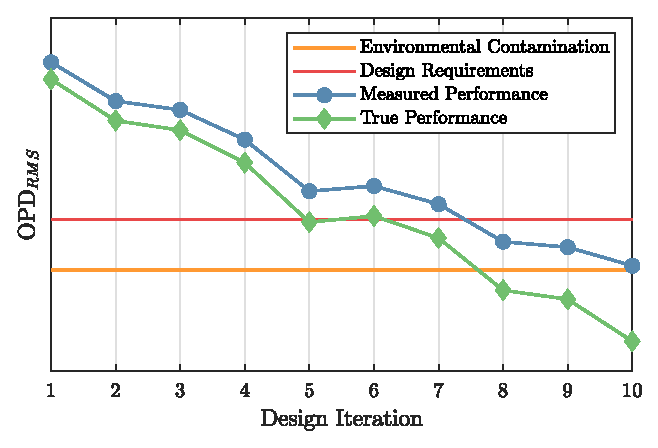
\includegraphics{../matlab/01_introduction/design_iteration.eps}
  \caption{Hypothetical iterative design process of an airborne directed-energy system.  The required performance level is shown by the red line and the testing environment's contamination is shown by the orange line.}
  \label{fig:01_design_iteration}
\end{figure}

As the design process was simulated by an initial aero-optical $\opdrms$ shown on the left of the plot, and the improvement in system performance achieved with each design iteration was simulated as a nearly linear reduction in $\opdrms$ combined with 15\% random variation.
If only the measured data, that is, including the effect of environmental contamination using Equation \ref{eqn:01_combined_opd}, is used to assess the system's performance then three additional design iterations are needed to achieve a usable design, which can add significantly to the development time and costs.
If the environmental contamination is greater than the design requirement, the measured performance will never reach the required performance criteria.
However, if the environmental contamination can be estimated, mitigated and/or removed, then the measured performance is a more accurate evaluation of the true aero-optical performance, and design convergence can be achieved more quickly and with more accurate results.

This dissertation will examine the environmental contamination of aero-optical measurements in wind tunnels, with a particular focus on the contamination due to acoustic noise within the wind tunnel.
A review of the available literature and important concepts in given in Chapter \ref{chap:02_lit_review}.
In Chapter \ref{chap:03_optical_acoustics}, the optical disturbances caused by acoustic waves from simple plane and spherical waves are presented, leading to a process for estimating the acoustical environment within the test section of a wind tunnel.
The strength of an spherical acoustic wave will be assessed with both microphone and optical measurements.
Multi-dimensional spectral techniques will be used to analyze optical wavefronts in Chapter \ref{chap:04_dispersion} and to filter optical wavefronts in Chapter \ref{chap:06_single_filter}.
These filtering techniques will contain some optical contamination particularly in regions where the various signal components interfere with one another.
In order to further reduce the optical contamination, Chapter \ref{chap:07_multiple_filter} will utilize additional sensor information from both microphones and accelerometers to remove some of the overlapping contamination to obtain a better picture of the actual optical performance of an airborne directed-energy system from ground test measurements.

    % !TEX root = catron-dissertation.tex
\epstopdfsetup{outdir=./images/02_background/}

\chapter{Literature Review}
\label{chap:02_lit_review}

Strong narrow-band acoustic waves traveling upstream have been measured in-flight with optical wavefronts from a turret as part of the AAOL program \cite{DeLucca-2018-gBQdjTmT}.
This was one of the first indications that a temporally narrow-band acoustic signal related to a fan was a noise source that could contribute significantly to the overall signal.
Additional measurements have shown both narrow-band and broad-band acoustic signals measured in-flight through a flat window with both boundary and shear layers present \cite{Gordeyev-2020-6HnfJMnC}.
Broad-band acoustic signals have been reported previously in optical wavefront measurements during boundary layer measurements in wind-tunnels but the effect was only  important at low temporal frequencies \cite{Gordeyev-2014-jcJndkHM,Smith-2013-VXArwwux}.
Optical measurements have also been made looking specifically for the acoustic waves inside a wind-tunnel, by looking for narrow-band optical disturbances associated with the wind-tunnel fan, with various model support structures \cite{Catron-2018-DdVp6VZf}, or with acoustic duct modes, showing that the optical disturbances due to the acoustic environment not only travel upstream at $u-c$, but also downstream at $u+c$ and cross-stream at $\pm c$ \cite{Catron-2020-x8njYmmu}.

The literature review will consist of primarily two sections.
The first section will examine aero-optics while the second will look at acoustics inside of ducts.

\section{Aero-Optics}
In optically active flows the index-of-refraction, $n$, varies locally along with other fluid properties.
Gladstone and Dale \cite{Gladstone-1863-ND4wtDT9} found that the index-of-refraction of air is primarily a function of density with a loose dependence on the wavelength of light.
Gladstone and Dale proposed a ``specific refractive energy'' now known as the Gladstone-Dale constant, $K_{GD}$,
\begin{equation}
  K_{GD} = \frac{n-1}{\rho}\textrm{.}
  \label{eqn:02_gladstone_dale_constant}
\end{equation}
For air the refractive index can be related to state quantities \cite{Valley-1965-F3k3cmv6}
\begin{equation}
  n-1 = 77.6\times 10^{-6}\frac{p}{T}\left(1+\frac{7.53\times10^{-3}}{\lambda^2}\right)\textrm{,}
  \label{eqn:02_refractive_index_ptlambda}
\end{equation}
where $p$ is in mbar, $T$ is in K, and $\lambda$ is in $\mu$m.
By combining this relationship with the ideal gas law, the Gladstone-Dale constant can be determined as a function of light wavelength,
\begin{equation}
  K_{GD} = 2.23\times10^{-4}\left(1+\frac{7.53\times10^{-3}}{\lambda_{\mu m}^2}\right) \: \left[\frac{m^3}{kg}\right]\textrm{.}
  \label{eqn:02_gladstone_dale_wavelength}
\end{equation}
The Gladstone-Dale constant for air over the visible range is shown in Figure \ref{fig:02_gladstone_dale_wavelength}.
\begin{figure}
  \centering
  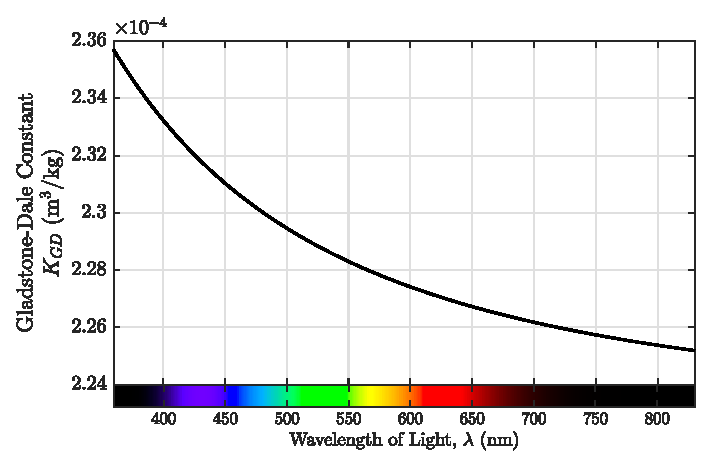
\includegraphics{../matlab/02_background/gladstone_dale_wavelength.eps}
  \caption{Gladstone-Dale constant for air over the visible wavelength range.}
  \label{fig:02_gladstone_dale_wavelength}
\end{figure}
While the value for $K_{GD}$ does vary over the visible range, it is only a few percent, and many sources use an average value of 2.27$\times10^{-4}$ m$^3$/kg for the visible and near-infrared \cite{Gardiner-1980-reW8xrCb}.
The Gladstone-Dale relationship is typically presented as
\begin{equation}
  n = 1+K_{GD}\rho
  \label{eqn:02_gladstone_dale_relation}
\end{equation}
but when applied to situations where there are significant fluctuations in the flow an alternate form is often more useful
\begin{equation}
  n'=K_{GD}\rho'
  \label{eqn:02_gladstone_dale_relation_fluctuating}
\end{equation}
where $'$ denotes the fluctuating component ($n' = n-\bar{n}$).

When a beam with an initially planar wave front passes through a region of optically active flow its wavefront becomes aberrated.
The optical path length ($\opl$) at any point in the beam can be obtained by integrating the index of refraction along the propagation of an optical ray \cite{Klein-1986-8Vx29RfE}.
\begin{equation}
  \opl (x,y,t) = \int^{s_2}_{s_1} n(x,y,z,t)ds
  \label{eqn:02_opl}
\end{equation}
The optical path difference ($\opd$), is then the spatially-averaged $\textrm{OPL}$ over an aperture removed from the OPL.
\begin{equation}
  \opd(x,y,t) = \opl(x,y,t)-\langle\opl(x,y,t)\rangle
  \label{eqn:02_opd}
\end{equation}
When working with fluctuating components, the $\opd$ can be calculated directly
\begin{equation}
  \opd(x,y,t) = \int^{s_2}_{s_1} n'(x,y,z,t)ds \textrm{.}
  \label{eqn:02_opd_n}
\end{equation}

As a finite beam of light travels normal to its wavefront it is diffracted, producing a theoretical limit on the performance of an optical system, i.e. diffraction-limited \cite{Born-1965-HHGYgjdH}.
Sommerfeld defined diffraction as ``any deviation of light rays from rectilinear paths which cannot be interpreted as reflection or refraction'' \cite{Sommerfeld-1954-ep2AWrFF}.
Diffraction through an aperture can be approximated with the Huygens-Fresnel principle by assuming that every point within the aperture produces a spherical wavelet \cite{Huygens-1690-gD8nxCn8},
\begin{equation}
  U(x_0,y_0) = \iint_{Ap} h(x_0,y_0;x_1,y_1)U(x_1,y_1)dx_1dy_1 \textrm{,}
  \label{eqn:02_huygens}
\end{equation}
where $U$ is the complex amplitude, the subscripts 0 and 1 represent the coordinates of the observation plane and aperture plane respectively, and
\begin{equation}
  h(x_0,y_0;x_1,y_1) = \frac{1}{j\lambda}\frac{\exp\{jkr_{01}\}}{r_{01}}\cos(\overrightarrow{n},\overrightarrow{r}_{01}) \textrm{,}
  \label{eqn:02_huygens_h}
\end{equation}
where $r_{01} = \sqrt{z^2+(x_0-x_1)^2+(x_0-y_1)^2}$, is the distance between any point in the observation and aperture planes.
Equation \ref{eqn:02_huygens} can be expanded to infinite limits of integration with the Kirchhoff boundary conditions where $U(x_1,y_1)$ is equal to zero outside of the aperture.
The obliquity factor, $\cos(\overrightarrow{n},\overrightarrow{r}_{01})$, can be approximated as being equal to one by assuming that the observation plane is at a much greater distance than the size of the aperture and is a small finite region.
The accuracy of this assumption is with 5\% if the angle between  $\overrightarrow{n}$ and $\overrightarrow{r}_{01}$ does not exceed $18^\circ$\cite{Goodman-1968-zPUmuuzx}.
With this assumption and for similar accuracy, $r_{01}$ in the denominator of Equation \ref{eqn:02_huygens_h} can be replaced with $z$, resulting in
\begin{equation}
  h(x_0,y_0;x_1,y_1) \approxeq \frac{1}{j\lambda z}\exp\{jkr_{01}\} \textrm{.}
\end{equation}

The Fresnel approximation replaces the spherical wavelets with a quadratic surface \cite{Fresnel-1818-FmMCMbDK},
\begin{equation}
  h(x_0,y_0;x_1,y_1) = \frac{\exp\{jkz\}}{j\lambda z}\exp\left\{j\frac{k}{2z}[(x_0-x_1)^2+(y_0-y_1)^2]\right\} \textrm{,}
  \label{eqn:02_fresnel_approx}
\end{equation}
which has a theoretical requirement that $z^3 \gg \frac{\pi}{4\lambda}\max\{[(x_0-x_1)^2+(y_0-y_1)^2]^2\}$ due to the limited number of terms used in a binomial expansion of $r_{01}$.
In practice this limit is not that critical \cite{Goodman-1968-zPUmuuzx}.
By combining Equations \ref{eqn:02_fraunhofer} and \ref{eqn:02_fresnel_approx}, an expression for Fresnel diffraction can be obtained,
\begin{equation}
  \begin{aligned}
    U(x_0,y_0) =& \frac{\exp\{jkz\}}{j\lambda z}\exp\left\{j\frac{k}{2z}(x_0^2+y_0^2)\right\}\iint_{-\infty}^{+\infty}\left[U(x_1,y_1)\exp\left\{j\frac{k}{2z}(x_1^2+y_1^2)\right\}\right] \\
    &\exp\left\{-j\frac{2\pi}{\lambda z}(x_0x_1+y_0y_1)\right\} dx_1dy_1 \textrm{.}
  \end{aligned}
  \label{eqn:02_fresnel}
\end{equation}
The function $U(x_0,y_0)$ may therefore be found from a two-dimensional Fourier transform:
\begin{equation}
  U(x_0,y_0) = \ft_2\left[U(x_1,y_1)\exp\left\{j\frac{k}{2z}(x_1^2+y_1^2)\right\}\right]
  \label{eqn:02_fresnel_fft}
\end{equation}
where $\ft_2$ is the two-dimensional Fourier transform and transform is evaluated at the spatial frequencies $\xi_x = x_0/\lambda z$, $\xi_y = y_0/\lambda z$.

The Fraunhofer approximation \cite{Goodman-1968-zPUmuuzx},
\begin{equation}
  z \gg \frac{k\max[x_1^2+y_1^2]}{2} \textrm{,}
  \label{eqn:02_fraunhofer_approx}
\end{equation}
places further restrictions than the Fresnel assumption approximation which results in
$\exp\left\{j\frac{k}{2z}(x_1^2+y_1^2)\right\}$ being approximately unity over the aperture further simplifying Equation \ref{eqn:02_fresnel} to
\begin{equation}
  \begin{aligned}
    U(x_0,y_0) =& \frac{\exp\{jkz\}}{j\lambda z}\exp\left\{j\frac{k}{2z}(x_0^2+y_0^2)\right\} \\
    &\iint_{-\infty}^{+\infty}U(x_1,y_1)\exp\left\{-j\frac{2\pi}{\lambda z}(x_0x_1+y_0y_1)\right\} dx_1dy_1 \textrm{.}
  \end{aligned}
  \label{eqn:02_fraunhofer}
\end{equation}
Equation \ref{eqn:02_fraunhofer} known as the Fraunhofer diffraction integral.
In Fraunhofer diffraction, the function $U(x_0,y_0)$ maybe found from the Fourier transform of $U(x_1,y_1)$, when evaluated at the spatial frequencies $\xi_x = x_0/\lambda z$, $\xi_y = y_0/\lambda z$.
For additional details on the derivation of Huygens, Fresnel, and Fraunhofer diffraction, including more in depth discussion on the assumptions and limits, see Goodman \cite{Goodman-1968-zPUmuuzx}.

The optical path difference can be related to the complex amplitude by \cite{Cicchiello-1997-RHxhNMxj},
\begin{equation}
  U(x_1,y_1) = \exp\left\{j\frac{2\pi}{\lambda}\opd(x_1,y_1)\right\} \textrm{.}
\end{equation}
Using the Fraunhofer diffraction integral, the nearfield $\opd$ disturbance can therefore be used to calculate the farfield intensity profile ($I = UU^*$),
\begin{equation}
  I(x_0,y_0) = \left|\ft_2\left(\exp\left\{j\frac{2\pi}{\lambda}\opd(x_1,y_1)\right\}\right)\right|^2 \textrm{,}
\end{equation}
where the transform is evaluated at the spatial frequencies $\xi_x = x_0/\lambda z$, $\xi_y = y_0/\lambda z$ in the observation plane and the complex amplitude outside of the aperture is zero.
For cases in which optical aberrations are nonexistent (i.e. $\opd(x,y,t)=0$), the farfield irradiance pattern that results from Equation \ref{eqn:02_fraunhofer} is caused entirely by diffraction from the optical aperture, and is referred to as the ``diffraction-limited'' irradiance pattern.
For a beam with a flat wave front and circular aperture, the farfield irradiance pattern is the Airy’s disk, and the peak irradiance at the center of the disk, $I_0$ , is the maximum irradiance that can be achieved by the optical system:
\begin{equation}
  I_0 = \left(\frac{kAp^2}{8z}\right)^2
  \label{eqn:02_airy_pattern}
\end{equation}
where $k$ is the wavenumber ($k=2\pi /\lambda$), $Ap$ is the aperture diameter, and $z$ is the distance from the aperture to the observation plane.
In the presence of aero-optical aberrations, $\opd(x,y,t)$ is non-zero, and the farfield irradiance pattern in this case tends to be more spread out and diffuse than the diffraction-limited case; furthermore, the beam may be shifted off target by optical tip/tilt imposed by the aberrations.

The Strehl ratio ($\sr$), is the ratio of intensity on target ($I$) to the diffraction-limited on target intensity ($I_0$):
\begin{equation}
  \sr=\frac{I}{I_0}
  \label{eqn:02_strehl_simple}
\end{equation}
The Strehl ratio can be computed accurately by applying Equation \ref{eqn:02_fraunhofer} twice, once for the diffraction-limited case to obtain $I_0$, and a second time with the $\opd$ field due to aero-optical aberrations included to obtain $I$.
The farfield performance, can also be estimated via the Mar\'{e}chal approximation:
\begin{equation}
  \sr(t) \equiv \frac{I(t)}{I_0} \approx \exp \left\{-\left[\frac{2\pi \opdrms(t)}{\lambda}\right]^2\right\}
  \label{eqn:02_strehl_ratio}
\end{equation}
where $\opdrms$ is the spatial rms of the wave front and $\lambda$ is the wavelength of the beam.
\begin{figure}
  \centering
  \begin{subfigure}[t]{0.45\textwidth}
    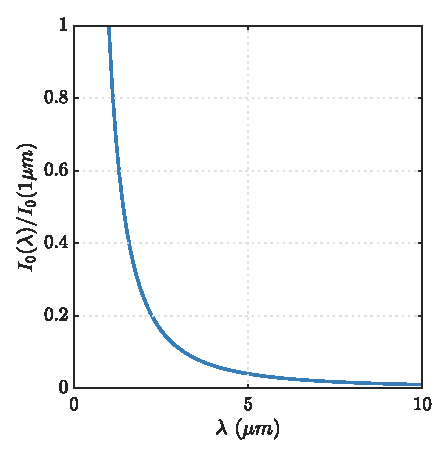
\includegraphics{../matlab/02_background/farfield_intensity.eps}
    \caption{}\label{fig:02_farfield_intensity}
  \end{subfigure}
  ~
  \begin{subfigure}[t]{0.45\textwidth}
    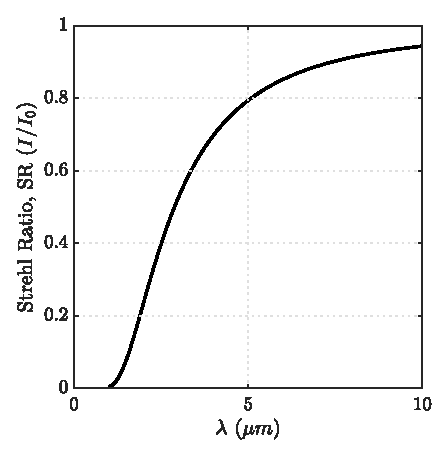
\includegraphics{../matlab/02_background/all_strehl_ratio.eps}
    \caption{}\label{fig:02_all_strehl_ratio}
  \end{subfigure}
  \caption{(\subref{fig:02_farfield_intensity}) Diffraction limited on target intensity as a function of wavelength normalized by the value at $\lambda$ = 1 $\mu$ m. (\subref{fig:02_all_strehl_ratio}) Strehl ratio as a function of wavelength for an aberration that gives SR = 0.95 at $\lambda$ = 10.6 $\mu$m.}
  % \label{FIG:airy_strehl}
\end{figure}
Equation \ref{eqn:02_strehl_ratio} reveals a key relationship between $\opd$, wavelength, and the farfield performance, plotted in Figure \ref{fig:02_all_strehl_ratio}, and shows that, for the same aero-optical aberration, the Strehl ratio decreases substantially as system wavelength decreases.
On the other hand, Equation \ref{eqn:02_airy_pattern} shows that the diffraction-limited farfield irradiance increases as the wavelength is shortened, plotted in Figure \ref{fig:02_farfield_intensity}.
Together, Figure \ref{fig:02_farfield_intensity} and \ref{fig:02_all_strehl_ratio} show that as modern optical systems move to shorter wavelengths to increase $I_0$, aero-optical aberrations cause a much more serious degradation of the Strehl ratio, illustrating why aero-optical considerations are critical in the development of new airborne optical systems.
Figure \ref{fig:02_necessary_opd} shows the $\opdrms$ necessary to achieve various Strehl ratios over a range of wavelengths.
\begin{figure}
  \centering
  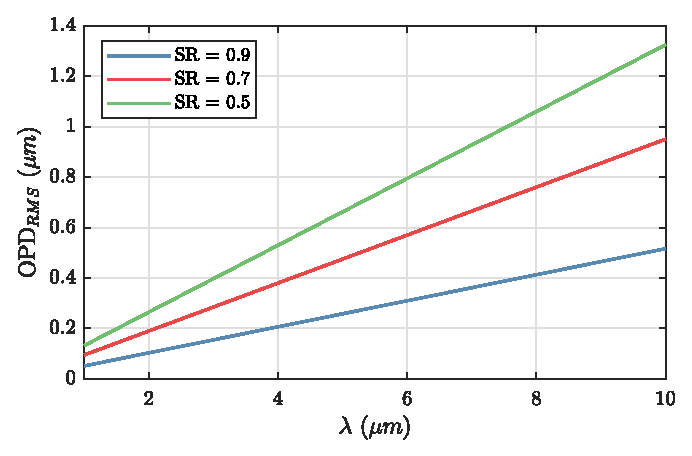
\includegraphics{../matlab/02_background/necessary_opd.eps}
  \caption{$\opdrms$ values necessary to obtain Strehl ratios of 0.9, 0.7, and 0.5 over a range of wavelengths.}
  \label{fig:02_necessary_opd}
\end{figure}
As the wavelength of light decreases the required $\opdrms$ decreases linearly for a fixed Strehl ratio.


\subsection{Typical Optical Wavefront Measurement System}
A diagram of a typical double-pass Shack-Hartmann wavefront front sensor setup is shown in Figure \ref{fig:02_typical_wavefront_system}.
\begin{figure}
  \centering
  \includegraphics[width=3.25in,clip,trim=170 75 170 75]{../cad/wavefront_setup.pdf}
  \put(-72,62){\rotatebox{90}{\Large LASER}}
  \put(-145,78){\rotatebox{90}{BEAM}}
  \put(-135,65){\rotatebox{90}{EXPANDER}}
  \put(-150,200){\rotatebox{90}{\Large PRIMARY TELESCOPE}}
  \put(-130,405){\rotatebox{90}{\Large MEASUREMENT}}
  \put(-112,432){\rotatebox{90}{\Large REGION}}
  \put(-95,160){\rotatebox{60}{\Large REIMAGING}}
  \put(-80,155){\rotatebox{60}{\Large TELESCOPE}}
  \put(-10,245){\rotatebox{90}{\Large WAVEFRONT}}
  \put(5,260){\rotatebox{90}{\Large SENSOR}}
  \put(-59,441){\fcolorbox{white}{white}{\Large $\gamma$}}
  \put(-90,480){\fcolorbox{white}{white}{\Large $\Longleftarrow$ Flow Direction}}
  \caption{Typical double-pass optical wavefront measurement setup.}
  \label{fig:02_typical_wavefront_system}
\end{figure}
The system starts with the laser in the bottom of the plot, which is then expanded to a larger diameter.
The beam expander used in this research increased the diameter of the beam to approximately 1-inch.
The larger diameter beam then passes through a beam splitter where half of the intensity is discarded and the other half proceeds to the primary telescope.
The primary telescope expands the beam to the desired size for the first passage through the measurement region.
For measurements made in a wind-tunnel, the beam angle, $\gamma$, is typically defined based on the flow direction \cite{Gordeyev-2014-jcJndkHM} with $0^\circ$ being looking straight into the flow and $180^\circ$ looking downstream.

A large mirror is used to return the beam along the same path for a second passage through the measurement region where the primary telescope shrinks the beam back down to a 1-inch diameter.
On the return path, the beam splitter sends half of the intensity back through the beam expander to the laser and half to the reimaging telescope.
The reimaging telescope serves two purposes, the first is to create an image plane for the wavefront sensor at the desired object plane location, typically the return mirror for a double-pass setup.
The second is to reduce the beam diameter for the wavefront sensor to a size that depends on the resolution and frame rate needed for a measurement.

The Shack-Hartmann wavefront sensor is comprised of a lenslet array and a camera \cite{Geary-1995-TQXWWFW2}.
A diagram of how the wavefront sensor functions can be seen in Figure \ref{fig:02_lenslet_array}.
\begin{figure}
  \centering
  \includegraphics[width=0.8\textwidth]{../other-sources/Shack_Hartmann_WFS_lensletarray.png}
  \caption{Diagram of a Shack-Hartmann wavefront sensor comprised of four lenslets. The black line represents the perturbed wavefront and the red line the mean slope over each lenslet. The focal point of the wavefront is shifted by $\Delta x$ from the center-line of the lenslet based on the mean slope of the wavefront. \cite{Shack-Hartman-Diagram-Wikipedia}}
  \label{fig:02_lenslet_array}
\end{figure}
The perturbed wavefront is represented by the black lines on the top of the figure.
Each lenslet produces a focused spot on the image plane with a location given by the average slope of the portion of the wavefront that passes through the lenslet.
By measuring the displacement, \cite{Nightingale-2013-gqr4p7GY}, of the focal dot from its normal position, the average slope, $\theta_x$ and $\theta_y$, of the wavefront over a lenslet can be measured,
\begin{equation}
  \theta_x = \tan^{-1}{\frac{\Delta x}{f}} \approx\frac{\Delta x}{f} \textrm{,}
\end{equation}
where $f$ is the focal length of the lenslet.
With an array of gradient data, the optical path difference at each lenslet can be calculated using a number of integration methods \cite{Huang-2015-W29DqPyp}, for example, one well-known method is the Southwell method \cite{Southwell-1980-KqUZMXRB}.

\subsection{Boundary Layer Optical Distortions}
\label{sect:02_BL_OPD}
Because optical wavefront measurements within a wind tunnel will usually include the optical distortion from the boundary layer(s) on the wind-tunnel wall(s), it is important to have some familiarity.
The time-averaged optical disturbance for a large aperture has been reported as,
\begin{equation}
  \opdrms = B(\gamma)K_{GD}\rho_\infty M^2\delta\sqrt{C_f}G(M) \textrm{,}
  \label{eqn:02_opdrms_gor}
\end{equation}
where $C_f$ is the skin-friction coefficient.
The function $B(\gamma)$ accounts for angle between the beam and the direction of flow, $\gamma$:
\begin{equation}
  B(\gamma) = \frac{0.19}{\sin(\gamma)} \textrm{,}
\end{equation}
and
\begin{equation}
  G(M) = 1-0.19M^2+0.03M^4 \textrm{.}
\end{equation}
Aperture size can be accounted for by Figure \ref{fig:02_gordeyev_2014} (Figure 18 in Gordeyev \cite{Gordeyev-2014-jcJndkHM}) with an approximation for the fit,
\begin{equation}
  \frac{\opdrms(Ap)}{\opdrms} \approx 1-a\exp\left\{b\frac{Ap}{\delta}\right\}-(1-a)\exp\left\{c\frac{Ap}{\delta}\right\} \textrm{,}
  \label{eqn:02_opdrms_gor_fit}
\end{equation}
where $a=0.7795$, $b=-0.9616$, and $c=-0.1382$.
\begin{figure}
  \centering
  \includegraphics[width=0.75\textwidth]{../other-sources/gordeyev_2014_figure_18.png}
  \caption{Aperture size correction for $\opdrms$ (Figure 18 in Gordeyev \cite{Gordeyev-2014-jcJndkHM}).}
  \label{fig:02_gordeyev_2014}
\end{figure}

\section{Duct Acoustics}
This section will look at acoustics when confined to a duct in which the acoustic waves primarily travel in the direction of one axis and have walls confining the acoustics along the other two axes as is the case inside of a wind tunnel.
Figure \ref{fig:02_duct_drawing} shows the diagram used for deriving the acoustic properties inside of a constant area duct.
\begin{figure}
\centering
    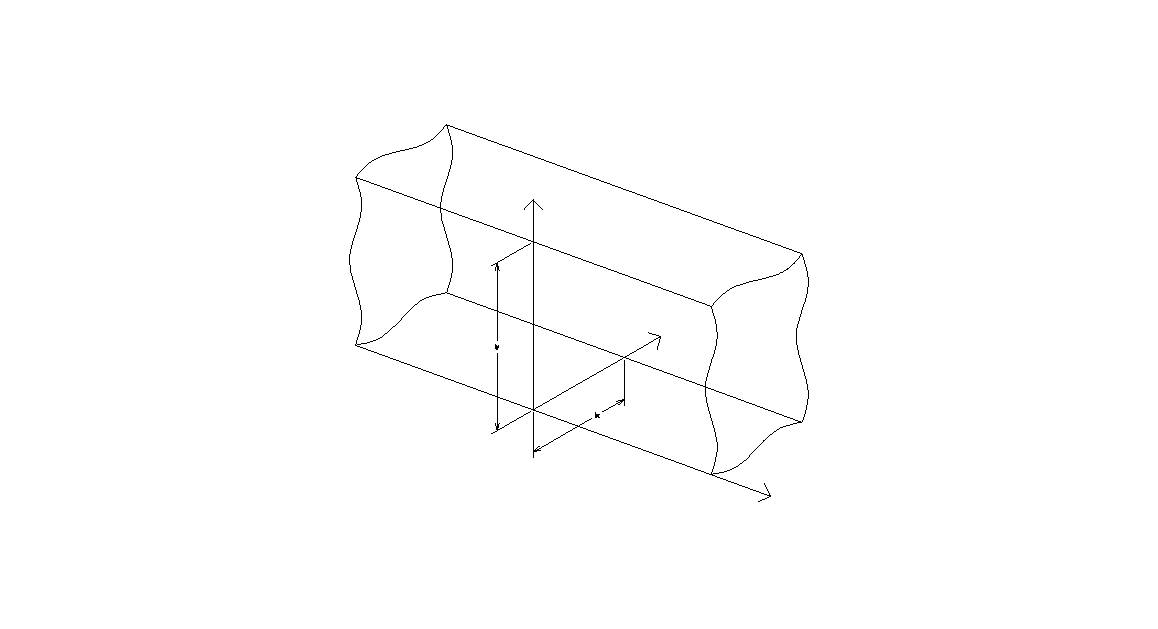
\includegraphics[trim=2.2in 0.7in 2.2in 0.7in,clip,width=4.5in]{../autocad/02_background/duct_drawing.eps}
    \put(-155,62){\fcolorbox{white}{white}{$l_x$}}
    \put(-227,113){\fcolorbox{white}{white}{$l_y$}}
    \put(-103,119){$\mathbf{x}$}
    \put(-198,220){$\mathbf{y}$}
    \put(-26,4){$\mathbf{z}$}
  \caption{Duct with a rectangular cross-section.}
  \label{fig:02_duct_drawing}
\end{figure}

The derivation presented here is primarily influenced by Munjal \cite{Munjal-2014-w28y4EyP} along with Jacobsen and Juhl \cite{Jacobsen-2013-PHD3v3YZ}.
The assumption used in this derivation is that the duct is of constant cross-section;
methods used to solve for the acoustic field in a wind tunnel with varying flow cross sections are presented later in Section \ref{sect:03_test_section}.
This means that all mean quantities ($\rho_0$, $\mathbf{u_0}$, ...) are constant throughout space and time.
Starting with the linearized inviscid forms of the conservation of mass,
\begin{equation}
  \frac{\mathbf{D}\rho}{\mathbf{Dt}} + \rho_0\nabla\cdot\mathbf{u} = 0 \textrm{,}
  % \frac{\partial\rho}{\partial t} + \mathbf{u}\cdot\nabla\rho + \rho_0(\nabla\cdot\mathbf{u}) = 0 \textrm{,}
  \label{eqn:02_cons_mass}
\end{equation}
and conservation of momentum,
\begin{equation}
  \rho_0\frac{\mathbf{Du}}{\mathbf{Dt}} + \nabla p = 0 \textrm{.}
  % \rho_0\frac{\partial\mathbf{u}}{\partial t} + \rho_0(\mathbf{u_0}\cdot\nabla)\mathbf{u} + \nabla p = 0 \textrm{.}
  \label{eqn:02_cons_mom}
\end{equation}
The definition of the speed of sound ($\left.\frac{\partial p}{\partial\rho}\right|_s = c_0^2$) is then substituted into Equation \ref{eqn:02_cons_mass},
\begin{equation}
  \frac{1}{c_0^2}\frac{\mathbf{D}p}{\mathbf{Dt}} + \rho_0\nabla\cdot\mathbf{u} = 0 \textrm{,}
  % \frac{1}{c_0^2}\frac{\partial p}{\partial t} + \frac{1}{c_0^2}(\mathbf{u}\cdot\nabla p) + \rho_0(\nabla\cdot\mathbf{u}) = 0 \textrm{,}
  \label{eqn:02_cons_mass_p}
\end{equation}
where $c_0$ is the speed of sound at average fluid properties ($\rho_0$, $p_0$, $T_0$, ...).
Next the difference between the material derivative ($\mathbf{D}/\mathbf{Dt}$) of Equation \ref{eqn:02_cons_mass_p} and the partial derivative ($\partial/\partial\mathbf{x}$) of Equation \ref{eqn:02_cons_mom} with respect to space is taken which results in the convected 3-D wave equation,
\begin{equation}
  \left(\frac{\mathbf{D}^2}{\mathbf{Dt}^2}-c_0^2\nabla^2\right)p=0\textrm{.}
  \label{eqn:02_wave_conv_3_c}
\end{equation}
Expanding the material derivative and dividing by $c_0^2$,
\begin{equation}
  \left(\frac{1}{c_0^2}\frac{\partial^2}{\partial t^2} + \frac{2\mathbf{M}}{c_0}\frac{\partial^2}{\partial t\partial\mathbf{x}} - (1-\mathbf{M}^2)\nabla^2\right)p = 0 \textrm{,}
  \label{eqn:02_wave_conv_expand}
\end{equation}
where $\mathbf{M} = \mathbf{u_0}/c_0$.
By using the fact that $c_0=\omega/k_0$, Equation \ref{eqn:02_wave_conv_3_c} can be written in a more convent form,
\begin{equation}
  \left(\frac{1}{\omega^2}\frac{\partial^2}{\partial t^2} + \frac{2\mathbf{M}}{\omega k_0}\frac{\partial^2}{\partial t\partial\mathbf{x}} - \frac{1-\mathbf{M}^2}{k_0^2}\nabla^2\right)p = 0 \textrm{,}
  \label{eqn:02_wave_conv_3}
\end{equation}
where $\omega$ is the angular frequency and $k_0$ is the total wavenumber.

At this point the pressure field is written in complex form and assumed to be separable in both time and space such that $\hat{p}(\mathbf{x},t) = \hat{p}(x,y)\hat{p}(z)\hat{p}(t)$.
The temporal solution is assumed to take the form
\begin{equation}
  \hat{p}(t) = \exp\left\{j\omega t\right\} \textrm{,}
  \label{eqn:02_pressure_solution_time}
\end{equation}
which results in the spatial component of the convecting wave equation
\begin{equation}
  \left((1-\mathbf{M}^2)\nabla^2-2jk_0\mathbf{M}\nabla+k_0^2\right)\hat{p}(x,y)\hat{p}(z) = 0 \textrm{.}
  \label{eqn:02_wave_conv_space}
\end{equation}
This can be further split into axial and cross-sectional components by splitting $k_0$ into components,
\begin{equation}
  k_0 = \sqrt{k_{xy}^2+k_z^2} \textrm{,}
  \label{eqn:02_k0}
\end{equation}
and because the mean flow is only in the axial direction ($\mathbf{M} = M\mathbf{\hat{k}}$).
The cross-sectional component is a typical Helmholtz equation
\begin{equation}
  \left(\frac{\partial^2}{\partial x^2}+\frac{\partial^2}{\partial y^2}\right)\hat{p}_{xy}(x,y)+k_{xy}^2\hat{p}(x,y) = 0 \textrm{,}
  \label{eqn:02_wave_xy}
\end{equation}
whose solution,
\begin{equation}
  \hat{p}(x,y) = \Psi_m(x,y) \textrm{,}
  \label{eqn:02_pressure_solution_xy}
\end{equation}
is one of an infinite number of eigen-function solutions with discrete wavenumbers, $k_m$.
The axial component of the convecting wave equation,
\begin{equation}
  (1-M^2)\frac{\partial^2\hat{p}(z)}{\partial z^2} - 2jk_0M\frac{\partial\hat{p}(z)}{\partial z} + k_z^2\hat{p}(z) = 0 \textrm{,}
  \label{eqn:02_wave_z}
\end{equation}
retains the total wavenumber in the second term which means its solution will depend on the cross-sectional wavenumber value of the cross-sectional mode.
The solution to the axial convecting wave equation,
\begin{equation}
  \hat{p}(z) = C^+_m\exp{\left\{-jk^+_{zm}z\right\}}+C^-_m\exp{\left\{+jk^-_{zm}z\right\}} \textrm{,}
  \label{eqn:02_pressure_solution_z}
\end{equation}
has waves traveling in both directions with the axial wavenumber in each direction for a given mode
\begin{equation}
  k^\pm_{zm} = \frac{\mp Mk_0+\sqrt{k_0^2-(1-M^2)k_m^2}}{1-M^2} \textrm{.}
  \label{eqn:02_kzm}
\end{equation}

The solution for a three-dimensional acoustic wave in a duct with a constant but arbitrary cross-section in complex pressure is the combination of the component solutions presented in Equations \ref{eqn:02_pressure_solution_time}, \ref{eqn:02_pressure_solution_xy}, and \ref{eqn:02_pressure_solution_z},
\begin{equation}
  \hat{p}(x,y,z,t) = \Psi_m(x,y)\left(C^+_m\exp{\left\{-jk^+_{zm}z\right\}}+C^-_m\exp{\left\{+jk^-_{zm}z\right\}}\right)\exp\left\{j\omega t\right\} \textrm{.}
  \label{eqn:02_pressure_solution_duct}
\end{equation}
The two solutions for a plane wave ($\Psi_m=1$, $k_m=0$) traveling in a duct have a characteristic speed of $u\pm c_0$.
Acoustic modes will travel indefinitly if $k_0^2-(1-M^2)k_m^2>0$ (the quantity inside of the square-root of Equation \ref{eqn:02_kzm}).
This presents a frequency at which a given mode will cut-on,
\begin{equation}
  f_{cuton} = \frac{c_0}{2\pi}\sqrt{(1-M^2)k_m^2} \textrm{.}
  \label{eqn:02_cuton_freq}
\end{equation}
Below this frequency, an acoustic mode will be exponentially attenuated as it travels through the duct.

\subsection{Characteristic Equations of Cross-Sections}
In order to determine the characteristic equations of an acoustic field within a cross-section the solution to Equation \ref{eqn:02_wave_xy} needs to be determined.
In this research, it will be assumed that the walls of the duct are perfectly rigid, giving the following boundary condition for the 2-D Helmholtz equation:
\begin{equation}
  \nabla p_{x,y}(x,y)\cdot\mathbf{n}_{wall} = 0
  \label{eqn:02_bc_rigig_wall}
\end{equation}
This boundary condition results in the acoustic waves being perfectly reflected off of the duct walls.
There are several known empirical solution sets of the characteristic equations for specific geometries with the rigid wall assumption.

The first of these solutions is for a duct with rectangular cross-section,
\begin{equation}
  \Psi_{m,n}(x,y) = \cos(k_xx)\cos(k_yy) \textrm{,}
  \label{eqn:02_psi_rect}
\end{equation}
where the wave numbers along each axis are $k_x = m\pi/l_x$ and $k_y = n\pi/l_y$.
The duct has a width of $l_x$ and a height of $l_y$.
The total cross-sectional wave number for use in determining the axial wave numbers is
\begin{equation}
  k_m^2 = k_x^2+k_y^2 \textrm{.}
  \label{eqn:02_wave_number_crosssection}
\end{equation}
Figure \ref{fig:02_cross_section_rect} shows the characteristic functions when m=0:2 and n=0:3 for a rectangular cross-section of width of $l_x$ and height of $l_y$.
\begin{figure}
  \centering
  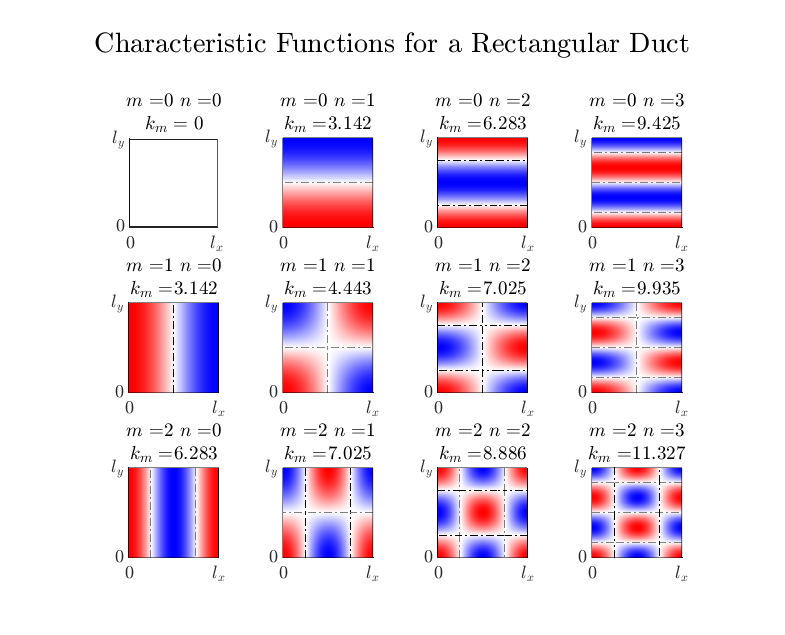
\includegraphics[width=\textwidth]{../matlab/02_background/cross_section_rect.eps}
  \caption{Characteristic solutions to Equation \ref{eqn:02_wave_xy} with rigid wall in a rectangular cross-section where m=0:2 and n=0:3.  Nodal lines are depicted by the dot-dash lines.  The cross-sectional wave numbers, $k_m$, listed are for a duct of unit length and height.}
  \label{fig:02_cross_section_rect}
\end{figure}
The lines depicted in the figure are nodal lines and represent locations where there is zero pressure fluctuations for that acoustic mode.

The second set of known empirical solutions is for a circular cross-section with radius $R$,
\begin{equation}
  \Psi_{m,n}(r,\theta) = J_m(k_{mn}r)\exp\left\{\pm jm\theta\right\} \textrm{,}
  \label{eqn:02_psi_circ}
\end{equation}
where $J_m$ is the $m^\textrm{th}$ Bessel function of the first kind and the $\pm$ indicates the direction of spin.
If the left and right spin coefficients are equal in magnitude then a non-spinning mode is created.
In order to satisfy the solid wall boundary condition $J_m'(k_{mn}R) = 0$ which determines a set of discrete values for the cross-sectional wave number at the $n^\textrm{th}$ zero for the $m^\textrm{th}$ Bessel function.
Figure \ref{fig:02_cross_section_circ} shows the characteristic functions for a circular duct.
\begin{figure}
  \centering
  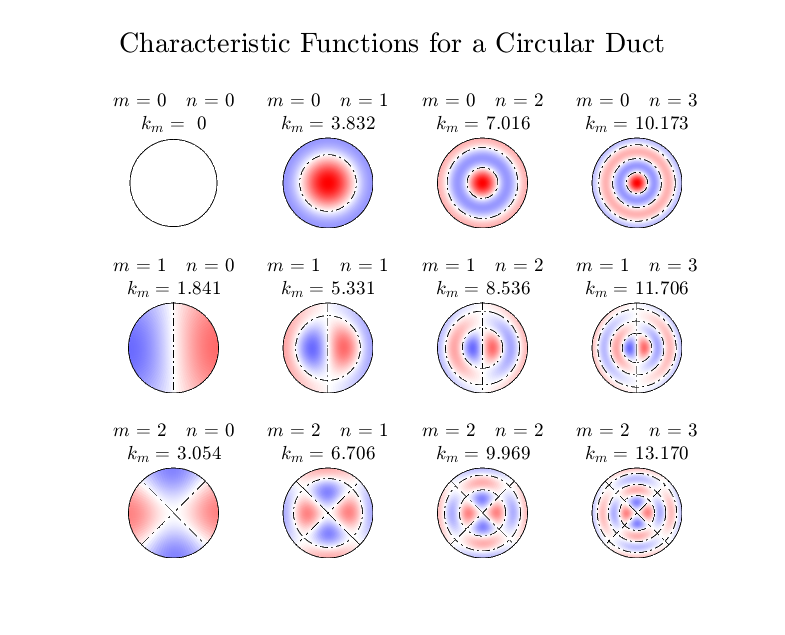
\includegraphics[width=\textwidth]{../matlab/02_background/cross_section_circ.eps}
  \caption{Characteristic solutions to Equation \ref{eqn:02_wave_xy} with rigid wall in a circular cross-section where m=0:2 and n=0:3.  Nodal lines are depicted by the dot-dash lines.  The cross-sectional wave numbers, $k_m$, listed are for a duct of unit radius.}
  \label{fig:02_cross_section_circ}
\end{figure}

    % !TEX root = catron-dissertation.tex
\epstopdfsetup{outdir=./images/03_aero_optics_acoustics/}

\chapter{Aero-Optical and Acoustical Coupling}

\begin{itemize}
  \color{red}
  \item Update plots to have constant nomenclature with the rest of the document
  \item Coordinate transform between beam and duct geometry
  \item Spherical solutions and measurements
  \item Mode marching method
\end{itemize}


Acoustic waves are isentropic compression waves with the fluctuating pressure, $p'$, determining the strength of the wave.
This fluctuating pressure is related to the sound pressure level, $\spl$ by
\begin{equation}
  \spl = 20\log_{10}\left(\frac{p_{rms}}{p_0}\right)
  \label{eqn:03_spl}
\end{equation}
where $p_{rms}$ is the root mean square of the pressure fluctuation, and $p_0$ is the reference pressure (20 $\mu$Pa for air).
The pressure fluctuations can be converted to the density fluctuations via the definition of the speed of sound:
\begin{equation}
  c_0^2 = \left(\frac{\partial p}{\partial \rho}\right)_s=\frac{p'}{\rho'}
  \label{eqn:03_speed_sound}
\end{equation}
where $c_0$ is the speed of sound at mean fluid properties and the subscript $s$ denotes constant entropy.
It can be shown by combining Equations \ref{eqn:02_gladstone_dale_relation_fluctuating} and \ref{eqn:02_opd} that the fluctuating density can be related to the $\opd$,
\begin{equation}
  \opd = K_{GD}\int_{s_1}^{s_2}{\rho'}ds \textrm{.}
  \label{eqn:03_opd_fluct}
\end{equation}
This can be combined with Equation \ref{eqn:03_speed_sound},
\begin{equation}
  \opd = \frac{K_{GD}}{c_0^2}\int_{s_1}^{s_2}{p'}ds \textrm{,}
  \label{eqn:03_opd_pressure}
\end{equation}
to provide a way of computing the optical path difference of a pressure field.

When the pressure field is known in complex quantities (magnitude and phase), a complex optical path difference can calculated,
\begin{equation}
  \widehat{\opd}(x,y) = \frac{K_{GD}}{c_0^2}\int_{z_1}^{z_2} \hat{p}(x,y,z)dz \textrm{.}
  \label{eqn:03_opd_complex}
\end{equation}
Here the complex pressure field was assumed to be seperable in time and space.
The measurable $\opd$ is
\begin{equation}
  \opd(x,y) = \real\left[\sum\widehat{\opd}(x,y)\exp\{j\omega t\}\right] \textrm{.}
  \label{eqn:03_opd_real}
\end{equation}
This can greatly reduce the computational cost of simulating a beam passing through a pressue or density field that is separable in time and space by only performing the spatial integration once for each temporal frequency component.

\section{Simple Examples of Acoustic-Optical Coupling}
Two basic acoustic pressure fields will be numerically examined for their optical properties.
The first will be a planar acoustic wave that will be numerically simulated over a variety of conditions.
The second will be a spherical acoustic wave that will be both numerically simulated and validated experimentally.

\subsection{Planar Acoustic Waves}
A planar wave is the simplest solution to the wave equation and varies only in time and the direction of travel.
A planar wave can be calculated from the set of solutions for duct acoustics, Equation \ref{eqn:02_pressure_solution_duct}, given that $\Psi_m(x,y)=1$,
\begin{equation}
  \hat{p}(z,t) = p_m\exp\left\{j(\omega t \mp k_{zm}^\pm z)\right\} \textrm{.}
  \label{eqn:03_plane_wave}
\end{equation}
This section will show several plots to show the effect that acoustic waves have on the optical wavefront of a planar wave with the general geometry shown in Figure \ref{fig:03_planar_sample_domain}.
\begin{figure}
  \centering
  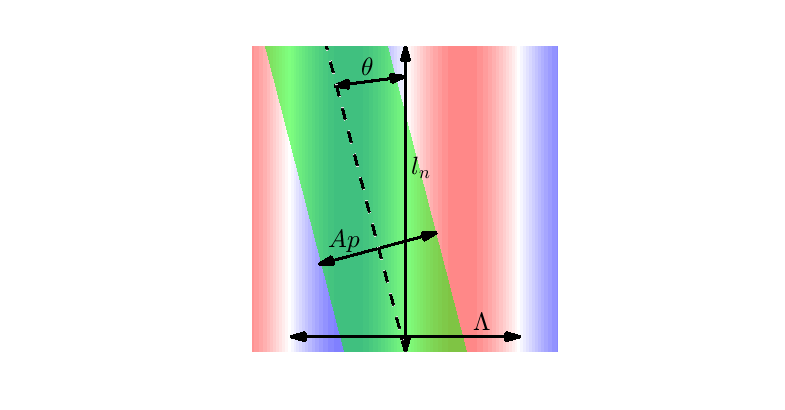
\includegraphics{../matlab/03_aero_optics_acoustics/planar_sample_domain.eps}
  \caption{General geometry for various sample calculations for showing the acoustic-optical coupling effect.}
  \label{fig:03_planar_sample_domain}
\end{figure}
For the following example, $l_n$ is the width of the acoustic disturbance (for example, the width of the wind tunnel), $\theta$ is the angle between the planar acoustic wave and the beam direction, $A_p$ is the aperture diameter of the beam, and $\Lambda$ is the wavelength of the acoustic wave.

Figure \ref{fig:03_planar_sample_calc_3} shows the time averaged $\opdrms$ per meter of beam propagation when the beam path is parallel ($\theta=0$) to the peaks and troughs of the planar acoustic wave as $\spl$ is varied.
\begin{figure}
  \centering
  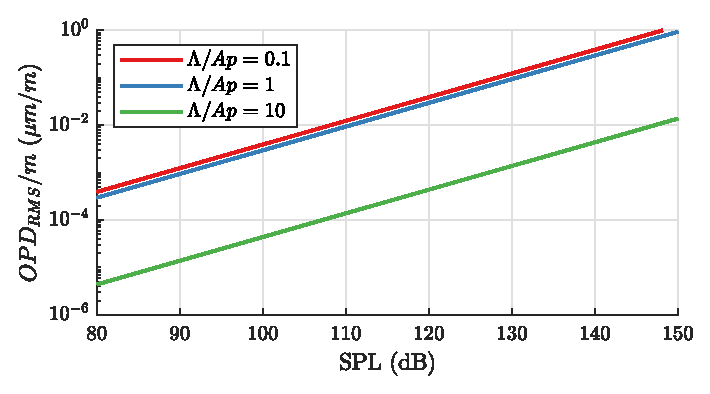
\includegraphics{../matlab/03_aero_optics_acoustics/planar_sample_calc_3.eps}
  \caption{Theoretical time-averaged $\opdrms$ per meter of beam propagation as a function of sound pressure level, $\spl$, for several $\Lambda/Ap$ ratios and $\theta=0$.}
  \label{fig:03_planar_sample_calc_3}
\end{figure}
As the sound pressure level increases the time averaged $\opdrms$ also increases and can easily reach the point of being a significant factor in the measured optical disturbance.
There is little difference between 0.1 and 1 $\Lambda/Ap$, but as the wavelength gets much larger compared to the beam diameter, then the optical effect of the noise is greatly reduced, this effect is known as aperture filtering \cite{Siegenthaler-2005-KQ2HGmfp}.

Aperture filtering is more clearly shown in Figure \ref{fig:03_planar_sample_calc_1}.
\begin{figure}
  \centering
  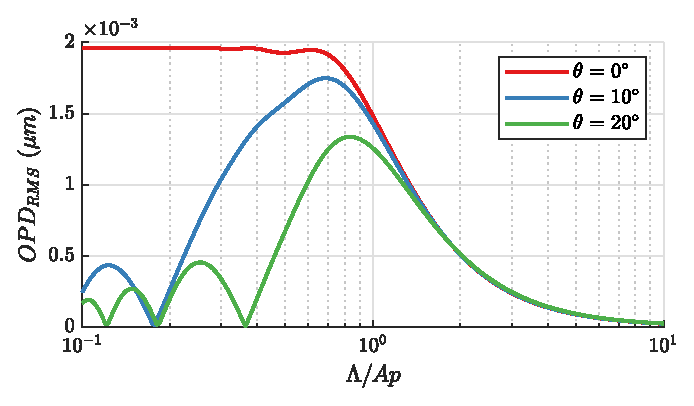
\includegraphics{../matlab/03_aero_optics_acoustics/planar_sample_calc_1.eps}
  \caption{Theoretical time-averaged $\opdrms$ for a rms sound pressure of 1 Pa ($\spl$ of 94 dB), $l_n$ of 1 m, and various angles and $\Lambda/Ap$ ratios.}
  \label{fig:03_planar_sample_calc_1}
\end{figure}
As the $\Lambda/Ap$ ratio increases from 0.1, time-averaged $\opdrms$ remains fairly constant until it starts to drop around $\Lambda/Ap$ of 0.7 and starts to asymptotically approach zero which it basically reaches by $\Lambda/Ap$ of 10.
Figure \ref{fig:03_planar_sample_calc_1} also shows the effect of changing the beam angle, $\theta$, through the acoustic field.
For nonzero $\theta$, the beam encounters alternating high and low index of refraction as it passes through the test region, so that the time-averaged $\opdrms$ begins to decrease compared to the $\theta = 0^\circ$ case below $\Lambda/Ap=1$.
There are also points of zero optical disturbance that occur at $\theta_{zero}=\tan^{-1}(n\Lambda/l_n)$ for $n\neq0$; these points occur because the peaks and valleys of the optical disturbance caused by the sound wave effectively cancel out over the length of the integration path, $l_n/\cos\theta$.

Figures \ref{fig:03_planar_sample_calc_3} and \ref{fig:03_planar_sample_calc_1} show the optical effect of plane acoustic waves in a no-flow environment.
The effect of wind-tunnel flow is to stretch (downstream-traveling waves) or compress (upstream-traveling waves) the wavelength of the acoustic noise thereby altering the filtering effect of the beam aperture.
Figure \ref{fig:03_planar_sample_calc_2} shows a typical optical disturbance from the two transverse acoustic waves (u+c and u-c) present in a wind tunnel at Mach 0.6.
\begin{figure}
  \centering
  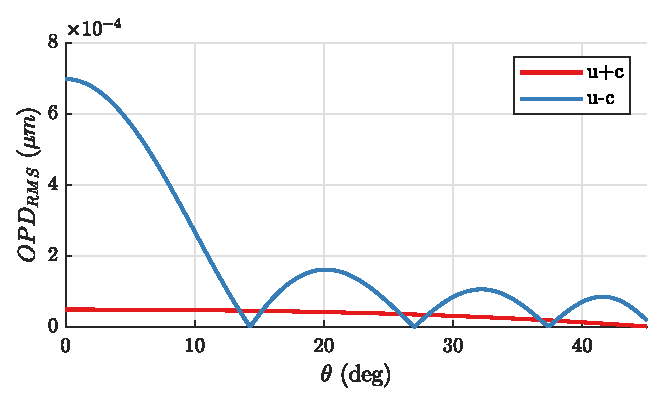
\includegraphics{../matlab/03_aero_optics_acoustics/planar_sample_calc_2.eps}
  \caption{Theoretical time-averaged $\opdrms$ for the two acoustic waves (u+c and u-c) for the blade pass frequency (534 Hz) at Mach 0.6 with a RMS sound pressure of 1 Pa ($\spl$ of 94 dB), $l_n$ of 1 m, and $Ap$ of 15 cm.}
  \label{fig:03_planar_sample_calc_2}
\end{figure}
Both waves have a RMS sound pressure of 1 Pa and the beam has an aperture of 15 cm and propagates through a 1 m acoustic field inside the tunnel.
Over a vast majority of the look back angles the upstream-traveling acoustic wave has a much greater effect on the optical disturbance compared to the downstream-traveling acoustic wave, due to the much shorter wavelength of the upstream-traveling waves which is less affected by aperture filtering.
However, the upstream-traveling wave goes through several zero points so the downstream-traveling wave dominates at some look back angles.

% In summary, Figures \ref{fig:03_planar_sample_calc_3} to \ref{fig:03_planar_sample_calc_2} give an example of how planar acoustic waves are expected to affect a beam traveling a finite distance $l_n$ at an angle $\theta$ through the acoustic field.

\subsection{Spherical Acoustic Waves}
The acoustic field from an speaker maybe assumed to be a spherical wave from a pulsating sphere if the frequency is sufficiently low and measurement region is far enough away from the source \cite{Randall-1951-9NtPPXPq}.

\begin{equation}
  \hat{p}(r,t) = \frac{A_0}{r}\exp\left\{-j(kr-\omega t)\right\}
  \label{eqn:03_spherical_pressure}
\end{equation}
% 3-16 pg61

\begin{equation}
  p_{rms} = \frac{|A_0|}{r\sqrt{2}}
  \label{eqn:03_spherical_pressure_rms}
\end{equation}

\begin{figure}
  \centering
  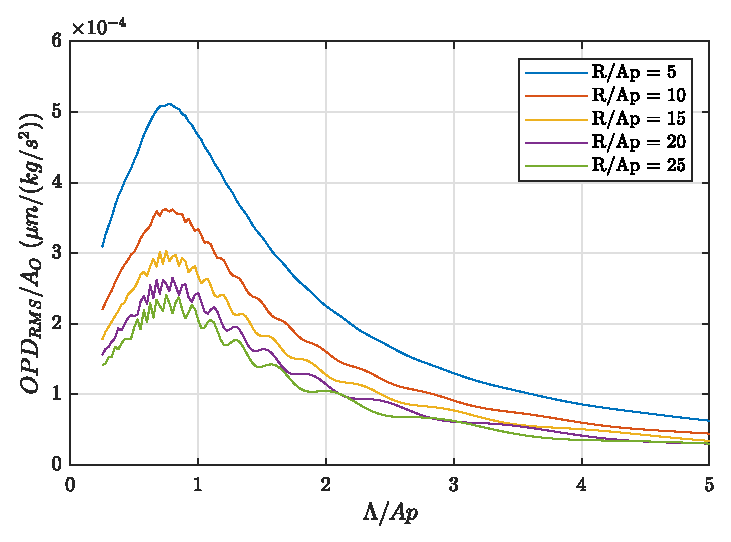
\includegraphics{../matlab/03_aero_optics_acoustics/spherical_sample.eps}
  \caption{Theoretical time-averaged $\opdrms$ for a spherical acoustic wave. There are oscillations not captured by the curve fit that are a function of aperture size.}
  \label{fig:03_spherical_sample}
\end{figure}

\begin{equation}
  \frac{\opdrms\sqrt{R/Ap}}{|A_0|} \approx \frac{p_1(\Lambda/Ap)^2+p_2(\Lambda/Ap)+p_3}{(\Lambda/Ap)^2+q_1(\Lambda/Ap)+q_2}
  \label{eqn:03_spherical_sample_fit}
\end{equation}


\begin{table}
\centering
\caption{Curve fit values for Figure \ref{fig:03_spherical_sample} and Equation \ref{eqn:03_spherical_sample_fit}}
\input{../matlab/03_aero_optics_acoustics/spherical_sample.txt}
\label{tab:03_speherical_sample_coeff}
\end{table}

\begin{table}
\centering
\caption{Comparison of microphone and wavefront computation of $|A_0|$}
\input{../matlab/03_aero_optics_acoustics/spherical_measurement.txt}
\label{tab:03_speherical_measurement}
\end{table}



\section{Estimating the Acoustic Field Inside the Test-Section}



\subsection{Mode Marching Process}
\begin{enumerate}
  \item Start with a known or assumed source acoustic field, $p^n(x,y)$

  \item Calculate the transmitted pressure ratio
  \begin{itemize}
    \item Traveling with subsonic flow
      \begin{equation}
        \frac{p^t}{p^i} = \left(\frac{1+M_n}{1+M_{n+1}}\right)\left(\frac{2M_{n+1}}{M_n+M_{n+1}}\right)\left(\frac{X_{n,n}}{X_{n,n+1}}\right)\left(\frac{X_{n,n}}{X_{n+1,n+1}}\right)^{1/(\gamma-1)}
      \end{equation}
    \item Traveling against subsonic flow
      \begin{equation}
        \frac{p^t}{p^i} = \left(\frac{1-M_n}{1-M_{n+1}}\right)\left(\frac{2M_{n+1}}{M_n+M_{n+1}}\right)\left(\frac{X_{n,n}}{X_{n,n+1}}\right)\left(\frac{X_{n,n}}{X_{n+1,n+1}}\right)^{1/(\gamma-1)}
      \end{equation}
    \item Where
      \begin{equation}
        X_{a,b} = 1+\frac{\gamma-1}{2}M_aM_b
      \end{equation}
  \end{itemize}

  \item March acoustic field to next axial step,
    \begin{equation}
      p^{n+1}(x,y) = p^{n}(x,y)\frac{p^t}{p^i}\exp\{j(\omega t\mp k_{zm}^\pm z)\}
    \end{equation}

  \item Best-fit set of local duct modes coefficients, $C_m$, to acoustic field $p^{n+1}(x,y)$

  \item Calculate new acoustic field from duct mode and repeat from step 2
    \begin{equation}
      p^n(x,y) = \sum_{m=0}^{M} C_m\cdot p_m(x,y)
    \end{equation}

  \item When the end point is reached, step inlet acoustic field (rotate fan) and repeat
\end{enumerate}

    % !TEX root = catron-dissertation.tex
\epstopdfsetup{outdir=./images/04_dispersion_analysis/}

\chapter{Dispersion Analysis}
\label{chap:04_dispersion}
\textcolor{red}{I think an analytical solution maybe needed for the n-dimensional case. Either a n-dimensional tophat function or dirac delta function. I also plan on adding a little analysis on viewing angle in the test-section.}

Dispersion analysis is an expansion of power spectra analysis from one-dimension to $n$-dimensions.
The technique allows a signal that is measured in both time and space to be separated into not only temporal-frequency components but also spacial-frequency components.
This allows not only the direction of travel that a particular wave to be determined but also the velocity of which that the wave travels.
The benefits of using a dispersion analysis are shown in Figure \ref{fig:04_dispersion_demo}.
\begin{figure}
\centering
  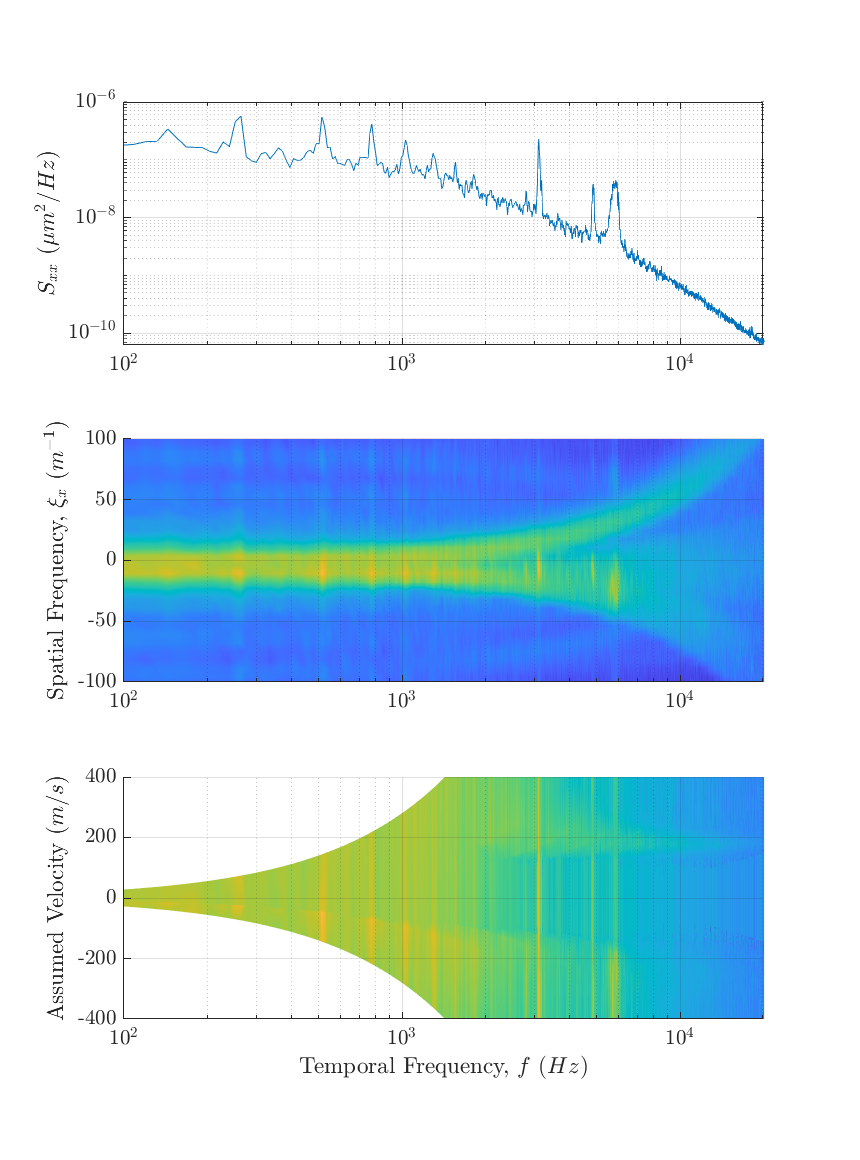
\includegraphics{../matlab/04_dispersion_analysis/dispersion_demo.eps}
  \caption{Dispersion plot example and comparison to traditional power spectra measurements. A single row of a wavefront measurement was used in this example. The top plot shows the typical power spectra measurement averaged over the entire row of data. Both the middle and bottom plots show the dispersion plot with the y-axis as spacial-frequency in the middle and velocity in the bottom assuming $u=f/\xi_x$.}
  \label{fig:04_dispersion_demo}
\end{figure}
The single row of sub-apertures from a wavefront measurement conducted with a 5-inch diameter beam propagating normally through two boundary layers with a free-stream Mach number of 0.5.
This measurement was preformed in the University of Notre Dame Whitefield Wind Tunnel in a test section that contained a model representing the fuselage of the AAOL aircraft \cite{Jumper-2013-8KtN3pue} with window that was flat and flush to the outer mold line of the fuselage.
The top plot shows a traditional power spectra representation averaged over the row of data.
Both the blade-passing frequency (517-Hz) and its sub-harmonic had similar power levels with an additional five harmonics showing significant spikes above the local baseline measurement.
There are three additional strong peaks at approximately 3100, 4850, and 5850 Hz that do not have an easily identifiable source or explanation.

Both the middle and bottom plots show a dispersion plot or two-dimensional power spectra measurement.
The colorbars were intentionally not shown in order to allow for all three plots to be aligned in the temporal frequency axis and the color space is representative of the power spectra in log-space.
The middle plot shows horizontally moving waves with the y-axis representing the spatial frequency, $\xi_x$, with units of inverse meters.
Waves with positive spatial frequencies are moving in the direction of flow.
All of the temporal frequency below 2000-Hz, where there is an obvious separation between the upstream and downstream traveling optical disturbances, are significantly more on the upstream traveling side.
The blade-passing frequency and its various harmonics show some significant broadband spatial frequency signals.
The three signals of unknown origin are clearly moving upstream but also show some significant broadband spatial signal that is indicative of a source producing optical disturbances that travel in both directions around the tunnel similar to the blade-passing frequency disturbances coming off of the wind tunnel fan.
In addition to optical disturbances branching off in the upstream and downstream moving directions there is a significant disturbances along zero spatial frequency representing a collection of standing waves.

The bottom plot shows the same dispersion plot as the middle one but with the y-axis representing an assumed velocity, $u_{assumed}$, where
\begin{equation}
  u_{assumed} = \frac{f}{\xi_x} \textrm{.}
  \label{eqn:04_velocity_assumed}
\end{equation}
The actual velocity, $u$, of a disturbance in the dispersion plot would be
\begin{equation}
  u = \frac{\partial f}{\partial \xi_x} \textrm{.}
  \label{eqn:04_velocity_actual}
\end{equation}
The assumed velocity measurement is in effect a average of the actual velocity assuming a zero-zero intercept in frequency space.
As there was no discernible separation between disturbance the upstream and downstream moving disturbances in the middle plot below 2000-Hz, there is no discernible velocity below that point.
The primary optical disturbance moving in the direction of flow is moving at the free-stream velocity of approximately 175-m/s.
The upstream traveling disturbance is traveling at the same speed but due to the signal being broader is more difficult to measure this way.
When the middle plot is shown with all linear axis, the slope of any given line through the origin is the inverse of the assumed velocity.
This is why the disturbances along the zero-spatial frequency line are a collection of standing waves and not some structure with broadband temporal content as it would be traveling at near infinite speed.
More discussion will follow a derivation of the dispersion analysis technique which is the n-dimensional power spectra.

\section{One-Dimensional Power Spectra Calculation}
The typical power spectrum calculation on a set of data that is only in one dimension, typically over the temporal dimension.
A typical example would be a single sensor measurement over time but a sensor array used to take data at one moment in time could used to measure the power spectrum in terms of spatial frequencies.
For a typical single-point measurement that varies in time, $x(t)$, the power spectra calculation is
\begin{equation}
 S_{xx} = \frac{|\fft(x(t))|^2}{N\cdot f_{s}} \textrm{,}
 \label{eqn:04_basic_sxx}
\end{equation}
where $\fft$ is the Fast Fourier Transform, $N$ is the number of samples, and $f_{s}$ is the sample rate \cite{Blackman-1958-4QtKgDb8}.
For data that has only a real component the Fast Fourier Transform function produces magnitude and phase relations at each frequency step, $f_{s}/N$, over the range from zero-frequency up to but not including the Nyquist frequency, $f_s/w$, with a mirrored set of data that can be represented either below (starting at $-f_s/2$) or above (ending just below $f_s$) this range.
The Nyquist frequency not being included and the mirrored data is due to an assumption that is integral to the Fourier Transform, that being the signal is assumed to be periodic.

The total energy, $\sigma^2$, of the signal must be preserved through the transform from physical space-time to frequency space
\begin{equation}
  \sigma^2 = \frac{\sum x^2(t)}{N} = \Delta f\sum S_{xx}(f) \textrm{.}
  \label{eqn:04_fft_energy_conservation}
\end{equation}
Additionally, because of the periodic nature of the Fourier Transform and a finite sample length of discrete data, spectral leakage can cause the power in one frequency bin to leak into adjacent frequency bins.
To minimize this spectral leakage, windowing functions are employed which typically force the end points of the signal to zero.
The Hann window,
\begin{equation}
 w(t) = 1/2\left[1-\cos\left(\frac{2\pi t}{T}\right)\right] \textrm{,}
 \label{eqn:04_hann_window}
\end{equation}
is one of the more commonly used windowing functions where $w(t)$ is the window function, $t$ is the time at a given sample, and $T$ is the total sample time.
Since the windowing of a data set changes the signal energy some correction is needed to be applied.
For an arbitrary windowing function the correction factor, $c_w$, can be obtained by substituting the windowing function in place of $x(t)$ in Equation \ref{eqn:04_fft_energy_conservation},
\begin{equation}
 c_w = \frac{1}{\sqrt{\sum w^2(t)/N}} \textrm{.}
 \label{eqn:04_window_correction}
\end{equation}
For a Hann window this correction factor approaches $\sqrt{8/3}$ as $N$ goes to infinity.
When Equation \ref{eqn:04_basic_sxx} is combined with a windowing function and associated correction the double sided power spectra equation in one dimension becomes
\begin{equation}
 S_{xx} = \cdot\frac{|c_w\cdot\fft\{x(t)\cdot w(t)\}|^2}{N\cdot f_{s}} \textrm{.}
 \label{eqn:04_windowed_sxx}
\end{equation}
A simple MATLAB function for computing the power spectrum of a one-dimensional signal with an arbitrary windowing function is shown in Appendix \ref{code:sc_simpleSXX}.

\section{N-Dimensional Power Spectra Calculation}
For measurements with multiple spatial and temporal dimensions the Fast Fourier Transform is applied $n$-times where $n$ is the total number of dimensions, with each application in a different dimension,
\begin{equation}
 \fftn(x) = \fft(\fft(\cdots\fft(\fft(x,1),2)\cdots,n-1),n) \textrm{,}
 \label{eqn:04_fftn}
\end{equation}
where $\fft(x,n)$ is the Fast Fourier Transform of $x$ in the $n^{th}$ dimension.
For a $n$-dimensional array the operation becomes,
\begin{equation}
 \mathbf{S_{xx}} =\frac{|c_w\cdot\fftn\{f(\mathbf{x})\cdot w(\mathbf{x})\}|^2}{\prod{\overrightarrow{N}\cdot\overrightarrow{f_s}}} \textrm{,}
 \label{eqn:04_sxxn}
\end{equation}
where $\mathbf{S_{xx}}$ is the $n$-dimensional power spectra array or dispersion array, $f(\mathbf{x})$ is a $n$-dimensional set of data, $w(\mathbf{x})$ is a $n$-dimensional windowing function, $\overrightarrow{N}$ is a vector denoting the number of elements in each dimension, $\overrightarrow{f_s}$ is a vector denoting the sample rate in each dimension, and
\begin{equation}
 c_w = \frac{1}{\sqrt{\sum w^2(\mathbf{x})/\prod{\overrightarrow{N}}}} \textrm{.}
 \label{eqn:04_windown}
\end{equation}
The signal energy conservation relationship becomes
\begin{equation}
  \sigma^2=\frac{\sum\mathbf{x}}{\prod{\overrightarrow{N}}} = \prod{\overrightarrow{\Delta f_s}}\sum\mathbf{S_{xx}} \textrm{,}
  \label{eqn:04_fftn_energy_conservation}
\end{equation}
where $\overrightarrow{\Delta f_s}$ is a vector representing the frequency step sizes in each dimension.
A simple MATLAB code for calculating the dispersion of $x$ with an arbitrary windowing function is shown in Appendix \ref{code:sc_simpleSXXn}.

\section{Non-Rectangular Spatial Windows}
For n-dimensional data sets that fill a rectangular array, a windowing function can easily be created by multiplying together a series of one-dimensional windowing functions created in the direction of each dimension.
For non-rectangular data sets, such as is often the case with optical wavefront measurement, windowing functions take some additional steps in there construction.
In cases when the spatial measurement locations are constant throughout time, the windowing function can be split into two separate components,
\begin{equation}
 w(\mathbf{x}) = w_t(t)\cdot w_s(x,y) \textrm{,}
 \label{eqn:04_window_sep}
\end{equation}
the temporal windowing function, $w_t(t)$, and the spatial windowing function, $w_s(x,y)$.
This dissertation uses a Hann window for the temporal windowing function and a modified Hann window for the spatial windowing function.
For the case of a circular aperture, the Hann window can be reformulated to be based normalized radius, $\rho_N$, of the aperture,
\begin{equation}
 w_s(\rho_N) =
 \begin{cases}
  \frac{1+\cos(\pi\cdot\rho_N)}{2} & \textrm{if } \rho_N < 1 \\
  0                                & \textrm{otherwise.}
 \end{cases}
 \label{eqn:04_window_space}
\end{equation}
This modified Hann window is two-dimensional with a value of one at the center of the aperture and decreases to zero at the edge of the aperture in the same manor as a Hann windows decreases from the center to either end.

Because the wavefronts measurements often had a clipped edge or some other obscuration, a different method was employed.
For an arbitrary shaped aperture, the minimum distance from any given measurement location to the edge of the aperture was used to create the spatial windows.
The minimum distance can be computed given the a set of points ($x$ and $y$) that spans the measurement range and the set of points outside of the aperture ($x_O$ and $y_O$),
\begin{equation}
 d_{min}(x,y) = \min\left\{\sqrt{(x-x_{O})^2+(y-y_{O})^2}\right\} \textrm{.}
 \label{eqn:04_window_space_arb_dist}
\end{equation}
This distance is then normalized by the maximum value and the resulting spatial window given a modified Hann window,
\begin{equation}
 w_s(x,y) = \frac{1+\cos\left\{\pi\cdot\left(1-d_{min}^{norm}(x,y)\right)\right\}}{2} \textrm{.}
 \label{eqn:04_window_space_arb}
\end{equation}
This same basic process can be extended to data sets where the locations of measurements in space vary with time.

\section{Dispersion Analysis}
At the beginning of this chapter a dispersion plot was shown along with a typical power spectra plot in Figure \ref{fig:04_dispersion_demo}.
This was for the purpose of doing a simple discussion of on some of the benefits of using a dispersion analysis on optical wavefronts.
That simple analysis was using only a single row of a wavefront and provided an incite into the disturbances that were moving in the horizontal direction only.
When a dispersion analysis is performed over all dimensions of a wavefront, as will be done for the remained of the chapter additional detail is available, additional detail as well as determination of optical disturbances moving vertically or any direction in between.
Figure \ref{fig:04_dispersion_comparison} shows a comparison between the two-dimensional single row dispersion and a three-dimensional dispersion showing the just the horizontal moving optical disturbances at both zero-vertical spatial frequency and the maximum value through all vertical spatial frequencies.
\begin{figure}
  \centering
  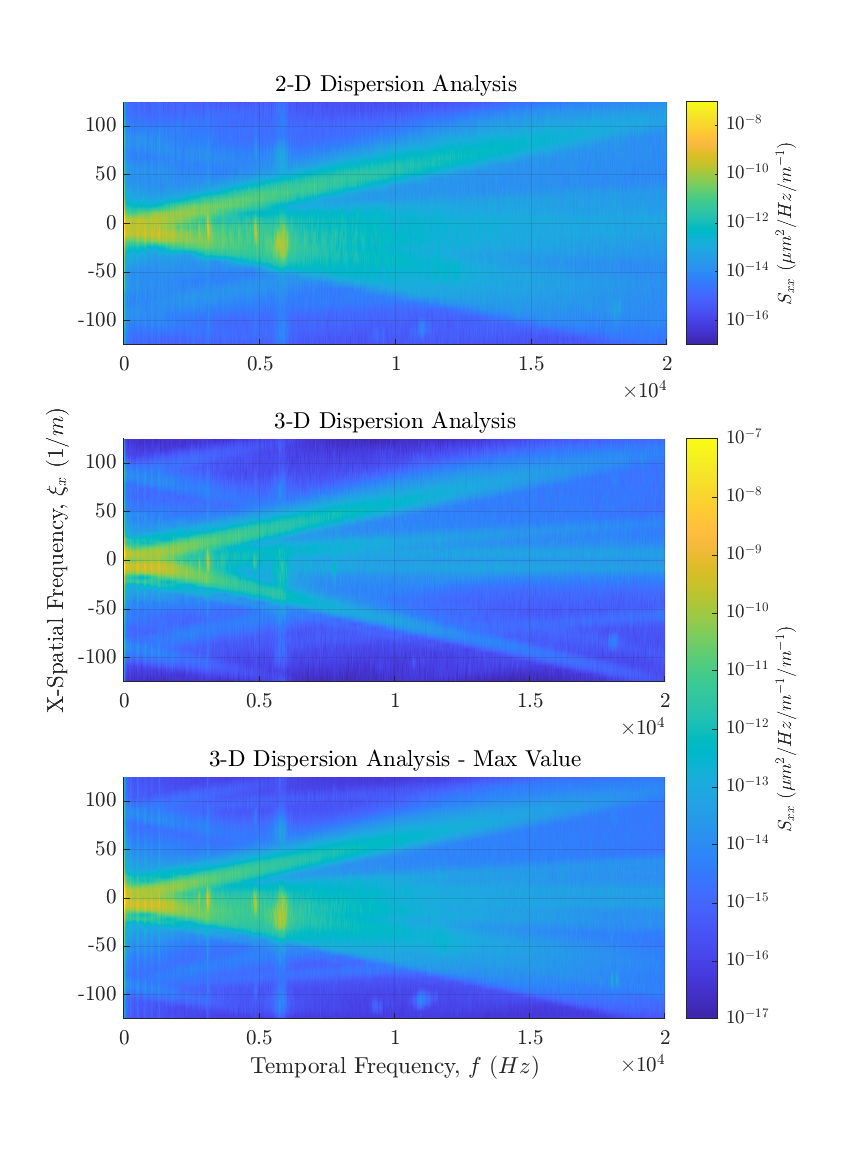
\includegraphics{../matlab/04_dispersion_analysis/dispersion_comparison.eps}
  \caption{Horizontal moving optical disturbances comparison. The top plot shows a two-dimensional dispersion analysis over a single row of data. The middle plot shows a three-dimensional dispersion analysis at $\xi_y=0$. The bottom plot shows the same three-dimensional dispersion analysis but showing the maximum value through the vertical axis.}
  \label{fig:04_dispersion_comparison}
\end{figure}
The top plots shows the two-dimensional dispersion plot that was previously shown in Figure \ref{fig:04_dispersion_demo} but this time with a linear temporal frequency axis.
The middle plot shows the three-dimensional dispersion plot at $\xi_y=0\ m^{-1}$, which shows a significant amount of additional data.
The two-dimensional dispersion shows a wide swath of signal that is generally traveling upstream from a line that goes through the origin and has a slight amount of positive slope downward to a line with a significant amount of negative slope.
This discussion of slopes is of the relative visible slope in the plots due and not actual slope calculation as the temporal frequency axis is several orders of magnitude larger than the spatial frequency axes (\textcolor{red}{footnote?}).

The slice of the full three-dimensional dispersion shows signal at the same limits for the two-dimensional swath of signal with some signal laying along the temporal frequency axis at $\xi_y=0\ m^{-1}$.
This signal represents a collection of stationary modes at each temporal frequency.
If this were to be some flow related phenomenon the velocity the disturbance would be nearing infinity.
On the three-dimensional dispersion plot there are easily observable signals that run parallel to the strongest signals but do not emanate from the origin.
These are signals that have been aliased due to the sample rate, either spatial or temporal, being to low.  This has some interesting implications in the possibility of being able to artificially increase the sample rate as will be discussed later.

The bottom plot of Figure \ref{fig:04_dispersion_comparison} shows the maximum value at each $f-\xi_x$ location through the range of $\xi_y$ values.
This effectively recreates the two-dimensional dispersion plot is a higher signal to noise ratio.
The aliased data is far more noticeable in this plot an in the two-dimensional one.
This indicates that a two-dimensional dispersion analysis is approximately the maximum value of the three-dimensional dispersion in a given dimension.
A reduced order dispersion can be calculated by
\begin{equation}
  S_{xx}^{n-1} = \max(S_{xx}^n,m)\cdot f_s^m \textrm{,}
\end{equation}
where $S_{xx}^n$ is the n-dimensional dispersion, $\max(x,m)$ is the maximum value of $x$ in the $m$-th dimension, and $f_s^m$ is the sample rate in the $m$-th dimension.
This can be shown in Figure \ref{fig:04_dispersion_max}.
The recovered power spectra from the two-dimensional dispersion analysis is a good estimation at the center of the frequency range but has some diversion near the edges.
It stays within half an order of magnitude below 1000-Hz with the signal peaks being a much closer approximation.
On the high end, the recovered power spectra has a decay rate that runs even with the direct computation up to about 10,000-Hz at which point the decay rate increases.
\begin{figure}
  \centering
  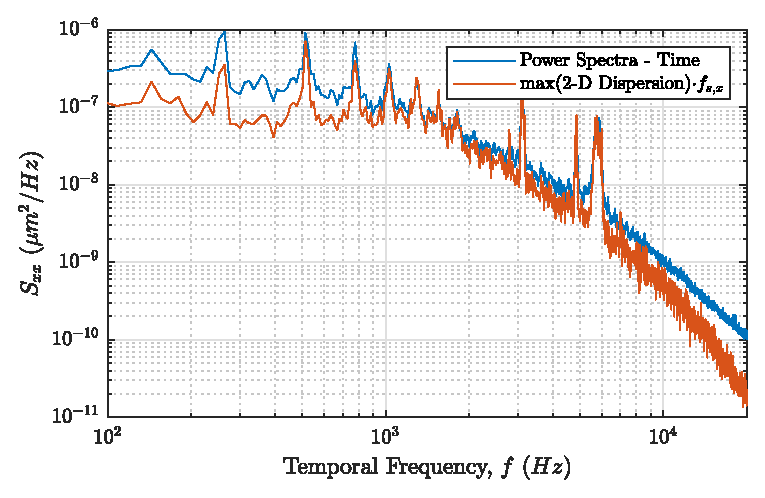
\includegraphics{../matlab/04_dispersion_analysis/dispersion_max.eps}
  \caption{Recovery of time-based power spectra from two-dimensional dispersion analysis.}
  \label{fig:04_dispersion_max}
\end{figure}

\subsection{2-D Slices of Full Dispersion}
The full dispersion analysis contains information of flow features not only moving in the horizontal direction as the two-dimensional dispersion showed but also in the vertical direction and the combinations of the two.
Figure \ref{fig:04_dispersion_xy} shows slices of the full dispersion in both the horizontal and vertical directions along with lines representing critical velocities.
Each of these plots is shown when the other spatial frequency is equal to zero, meaning that the disturbances shown are moving solely in that direction.
\begin{figure}
  \centering
  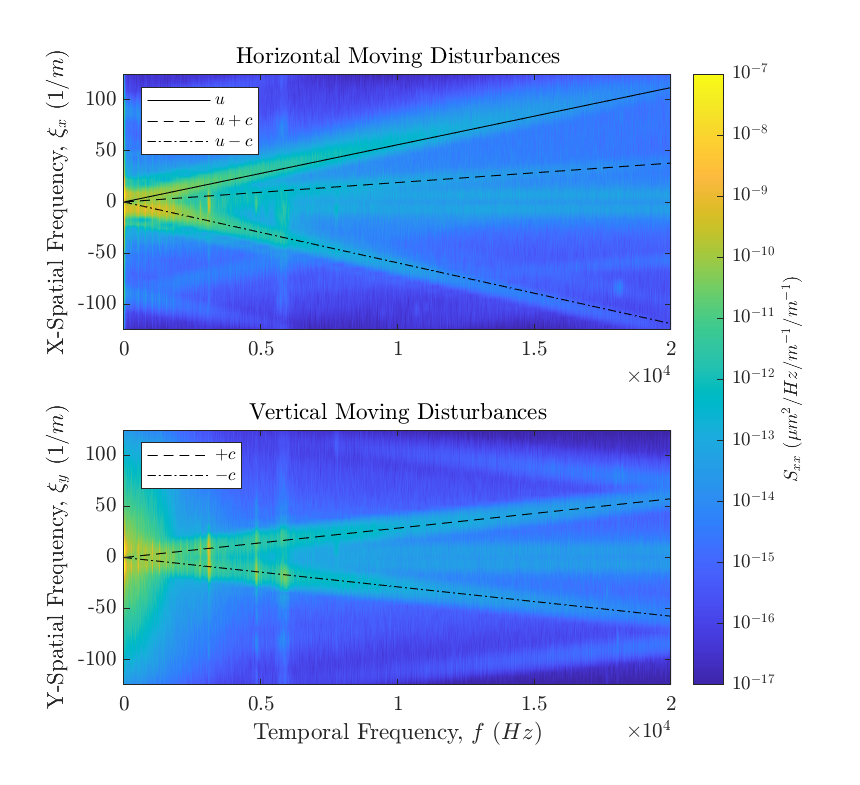
\includegraphics{../matlab/04_dispersion_analysis/dispersion_xy.eps}
  \caption{Horizontal and vertical moving optical disturbances. This is the same data as presented in Figure \ref{fig:04_dispersion_demo} but after calculating the full three-dimensional power spectra. The horizontal disturbances are shown at zero vertical spatial frequency and likewise the vertical disturbances are shown at zero horizontal spatial frequency.}
  \label{fig:04_dispersion_xy}
\end{figure}

The top plot shows the horizontally moving optical disturbances that has been shown previously.
There are three major flow related structures that can be observed.
The top most flow related structure is the boundary layers on both sides of the wind tunnel.
It can be seen that the boundary signal has a sharp drop off at the free-stream velocity, $u$, and has a slight decay as the velocity decreases (increasing slope).
Figure \ref{fig:04_dispersion_speed} shows the boundary layer velocity at a few cuts a little more clearly.
\begin{figure}
  \centering
  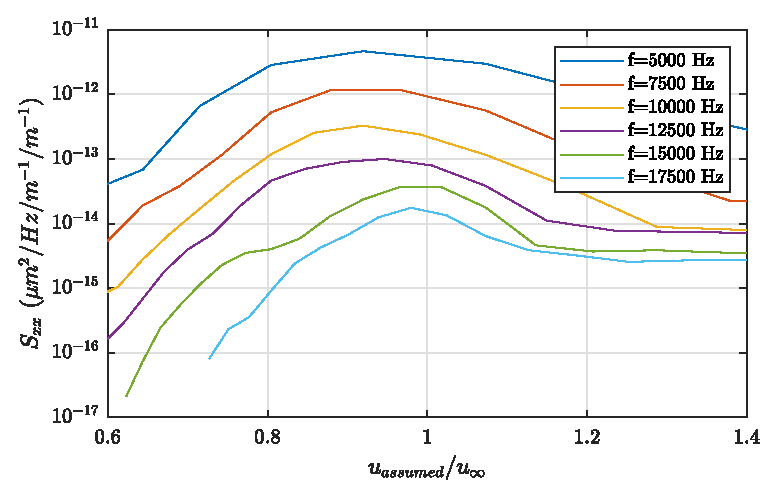
\includegraphics{../matlab/04_dispersion_analysis/dispersion_speed.eps}
  \caption{Assumed boundary speed at various temporal frequencies.}
  \label{fig:04_dispersion_speed}
\end{figure}
The boundary layer velocity has typically be reported as approximately 0.83$u$ \cite{Gordeyev-2014-jcJndkHM}.
This data shows the boundary layer velocity has a range of velocities at each given frequency in which the peak velocity component has some dependence on the temporal frequency.
The lower frequencies tend to have a lower velocity of around 0.9$u$ which is higher than has typically been reported while the higher frequencies approach the free-stream velocity.
When placing a lower bounding line on the boundary layer line in terms of speed in Figure \ref{fig:04_dispersion_xy}, a value of approximately 0.7$u$ seems to do a good job at bounding most of the boundary layer signal along with the free-stream velocity line.

The next two major flow related structures deal with acoustic signals traveling in both directions through the wind-tunnel.
The downstream traveling acoustic wave, $u+c$, typically has a low signal strength than the upstream traveling acoustic wave, $u-c$, due to the downstream traveling wave having a longer wavelength and thus more signal being filtered out due to aperture filtering \cite{Siegenthaler-2008-9Yutbt6c}.
At the low frequencies, the blade-passing frequency and its associated harmonics can be seen with regular spacing.
There also appears to be some constructive interference with the BPF and some of the aliased data around $\xi_x = \pm100\ m^{-1}$.

In both the horizontal and vertical moving plots the stationary modes are a prominent feature.
The two main features on the vertical moving disturbance plot is the signal at the speed of sound as well as some significant aliasing.
These to lines represent acoustic waves that are traversing either straight up or down.
Some of the high frequency spikes (~3, 5, and 6-kHz) seems to be laying along these speed of sound lines in the vertical direction and stationary in the horizontal direction.
These spikes maybe something in the test-section itself, along the top and bottom walls that is being excited and resonating.

\subsection{3-D Representations of Full Dispersion}
While the two-dimensional slices are fairly informative, particularly when it comes to signal strength of various flow structures and their velocities, a three-dimensional plot allows better visualization of the overall flow structures but some details are lost.
The same data that has been previously shown in slice form, is depicted in Figure \ref{fig:04_dispersion_3d} as an isosurface with a power of $10^{-14}$ $\mu m^2/Hz/m^{-1}/m^{-1}$ and shown from four different views.
\begin{figure}
  \centering
  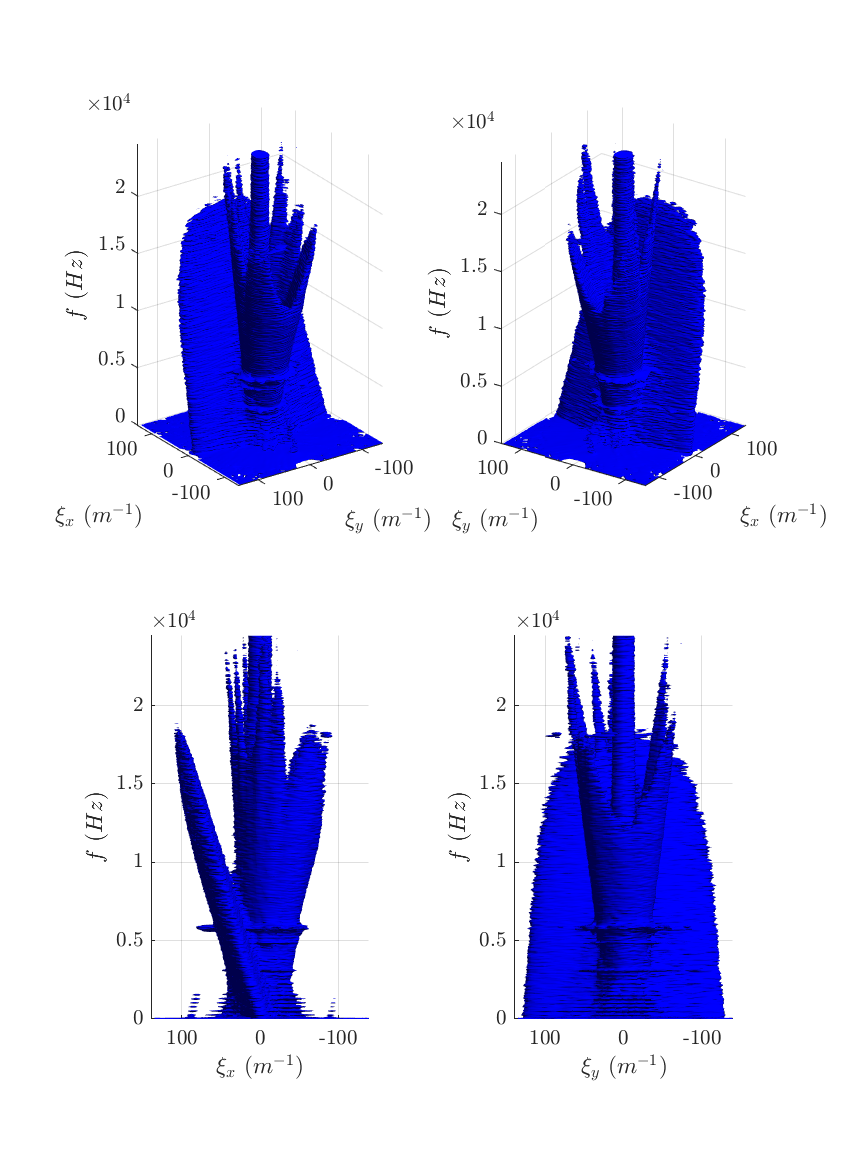
\includegraphics{../matlab/04_dispersion_analysis/dispersion_3d.eps}
  \caption{Three-dimensional view of the dispersion plot showing an isosurface at a power of $10^{-14}$ $\mu m^2/Hz/m^{-1}/m^{-1}$. The isosurface encompasses 99.9\% of the power of the wavefront.}
  \label{fig:04_dispersion_3d}
\end{figure}
This particular isosurface encompasses approximately 99.9\% of the power of the optical disturbances with little aliased information represented.
The largest feature is the boundary layer which resembles an ellipsoid or elliptical wing.
The other main feature is the acoustic signal which appears as a cone which has been tilted over a little bit.
The acoustic signal has several predominate spikes which form at high temporal frequencies indicating that there may be a small number of dominate duct modes.
The last feature is the stationary modes which have a near constant shape and magnitude through all frequency ranges.

Figure \ref{fig:04_dispersion_mach} shows two views of this three-dimensional dispersion but over a range of Mach numbers.
\begin{figure}
  \centering
  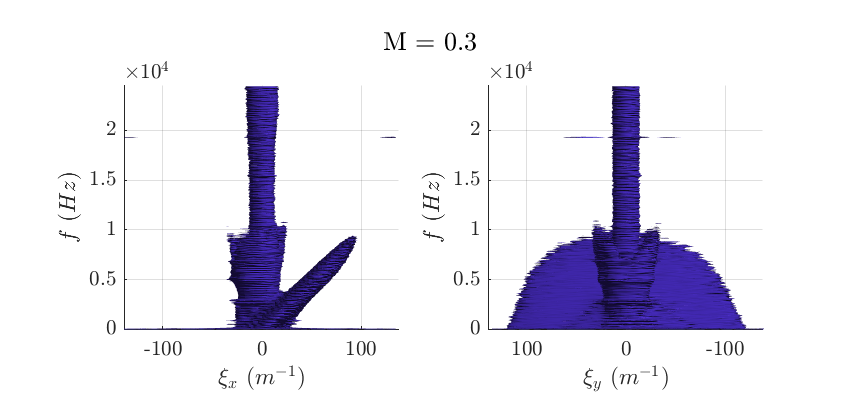
\includegraphics{../matlab/04_dispersion_analysis/dispersion_mach_0.3.eps}
  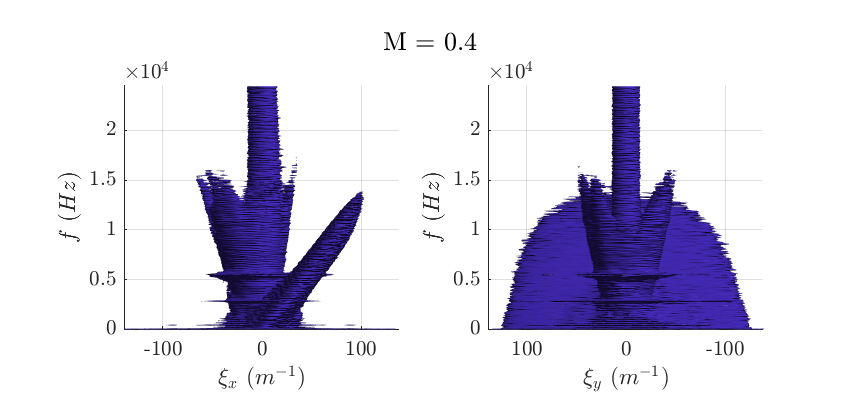
\includegraphics{../matlab/04_dispersion_analysis/dispersion_mach_0.4.eps}
  \includegraphics{../matlab/04_dispersion_analysis/dispersion_mach_0.5.eps}
  \caption{Three-dimensional view of dispersion plots as the Mach number increased from 0.3 to 0.5. The isosurfaces are all shown at a power of $10^{-14}$ $\mu m^2/Hz/m^{-1}/m^{-1}$ and all encompass 99.9\% of the wavefront power.}
  \label{fig:04_dispersion_mach}
\end{figure}
All of these plots are of an isosurface with the same strength as used in Figure \ref{fig:04_dispersion_3d}.
For a Mach number of 0.3, top plot, the most noticeable feature is the stationary modes which do not seem to change much as the Mach number is increase.
This indicates that the stationary waves are mostly as measurement artifact that could be from either laser or camera noise.
The boundary layer signal increases in power significantly as Mach number is increased but also the slope is significantly increased as well.
The acoustic signal sees some interesting evolution as well.
Along with the strength greatly increasing with Mach number, the slope of the upstream traveling disturbances decreases significantly while the downstream moving acoustic disturbances do not see much change other than an increase in signal strength.

While the three-dimensional views offer some significant incite, sometimes the insides need a close look a shown in Figure \ref{fig:04_dispersion_slices}.
\begin{figure}
  \centering
  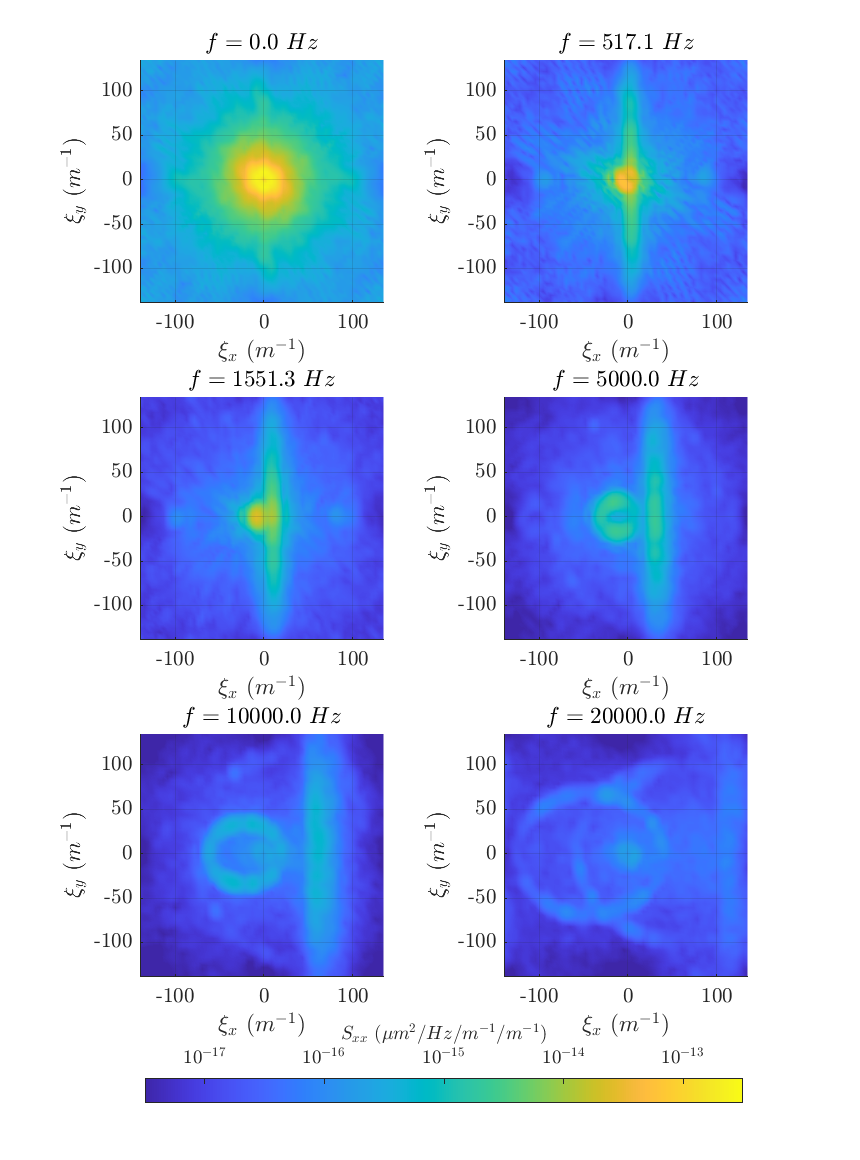
\includegraphics{../matlab/04_dispersion_analysis/dispersion_slices.eps}
  \caption{Additional dispersion slices at various temporal frequencies.}
  \label{fig:04_dispersion_slices}
\end{figure}
This figure shows slices of the dispersion array at several different temporal frequencies: a mean lensing slice at 0-Hz, the blade-passing frequency at 517-Hz, the second harmonic of the blade-passing frequency at 1551-Hz, and additional slices at 5, 10, and 20-kHz.
The mean lensing slice at 0-Hz shows a mostly axisymmetric pattern that is strongest in the center and dies out as the distance from the origin increases.
There appear to be the occasional spike radiating out from the center, most noticeably in line with the boundary layer signal.

The next four slices show boundary layers structure slowly moving towards positive x-spatial frequencies.
It does appear to be rotated slightly counter-clockwise indicating that the interrogation beam is slightly rotated between the test section and the wavefront sensor.
The boundary layers signal at the lower frequencies appears to be more elliptically shaped while the higher frequencies appear to have a sharp drop in signal strength going towards the origin and are slightly more feathered going away.
This could be indicative of lower frequency disturbances in the boundary layer typically traveling at a more uniform speed very near the free-stream velocity likely being either in the outer boundary layer or free-stream tunnel turbulence.
The higher frequency disturbances seem to have a wide range of velocities that approach the free-stream velocity and are likely small structures that span some significant portion of the boundary layer.

The acoustic disturbances show an interesting evolution as the frequency increase from fairly compact and strong signal just on the upstream traveling side of things around the blade-passing frequency to elliptical shaped rings at the higher frequencies.
At 20-kHz, there are two elliptical shapes that are easily identifiable, the smaller one is the signal that is actually present at that frequency while the other one is some aliased data due to a limited temporal sample rate.
The 10-kHz slice shows a little bit of acoustic aliasing
Both the 10 and 20-kHz acoustic rings show some favorable spatial frequencies which could also be seen in the three-dimensional view as spikes.
These two slices also show the center stationary modes that appear to be nearly identical.

\subsection{Artificially Increased Sample Rate}
Aliased data has been partially discussed previously.
When a signal crosses a plane represented by one of the Nyquist frequencies (positive or negative) it transposed to the conjugate Nyquist frequency plane and continues on with the same gradient as before, which is shown in Figure \ref{fig:04_dispersion_supersample} using the horizontal and vertical dispersion slices.
\begin{figure}
  \centering
  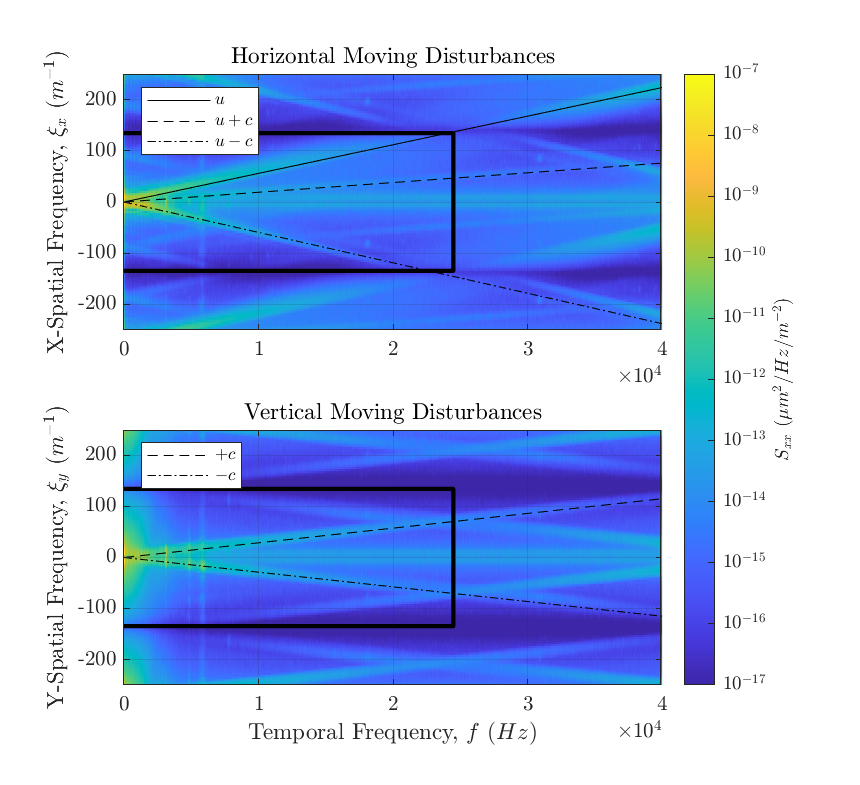
\includegraphics{../matlab/04_dispersion_analysis/dispersion_supersample.eps}
  \caption{Artificially increased temporal sample rate using a dispersion analysis. The black box represents original dispersion plot.}
  \label{fig:04_dispersion_supersample}
\end{figure}
Here the black box represents the original dispersion plot, while outside of that box is data that has an artificially increased sample rate.
This process can be accomplished by simply tiling the entire dispersion array in the desired dimension.
In this case the dispersion array was tiled in a three-by-three grid for each of the horizontal and vertical slices.
Along the spatial Nyquist frequency edges, there is a significant dip in the signal strength which would result in a spatial super sampling to have a significant loss of signal at these frequencies.

On the upstream moving disturbance side there is some noticeable aliasing that is present including a significant spike at 18-kHz (-80-$m^{-1}$) while aliased and about 31-kHz (-200-$m^{-1}$) when it has been unaliased.
As that upstream moving acoustic disturbance crosses the spatial Nyquist frequency, the signal strength drops significantly to local background levels.
The boundary layer signal is unfortunately to well aligned with its tiled self for any aliased data to be noticeable.
The vertically moving disturbances have some significant temporal aliasing but little to no spatial aliasing.

Just as the aliased signal is unaliased into the higher frequencies, non-aliased data is aliased into higher frequencies.
This means that some sort of filtering technique will need to be employed.
These filters should not only be designed to remove the aliased data from actual sample but also the aliased data from the super sampled frequencies.


% Depending of the sensor array construction, the signal could also be super sampled in the spatial dimensions as well.
% Because a Shack-Hartmann wavefront sensor is comprised of integrated measurements over each sub-aperture, artificially increasing the spatial sample rate is not possible due to the aperture filtering process.
%
% \begin{figure}
%   \centering
%   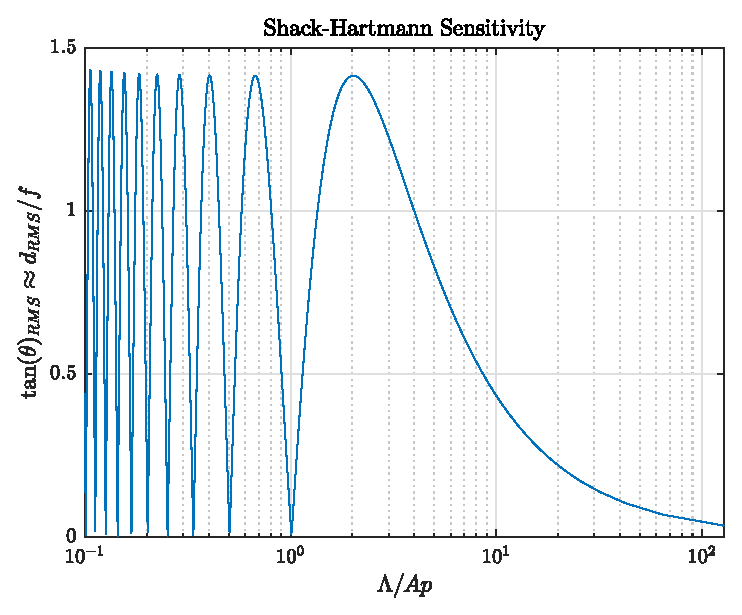
\includegraphics{../matlab/04_dispersion_analysis/shack_hartmann_sensitivity.eps}
%   \caption{Shack-Hartmann sensitivity as a function of the ratio of a structure's wavelength and the aperture size. This shows the RMS value of the displacement of the focal dot for a sub-aperture as a sinusoidal wave of unit magnitude passes through the sub-aperture.}
%   \label{fig:04_shack_hartmann_sensitivity}
% \end{figure}

    % !TEX root = catron-dissertation.tex
\epstopdfsetup{outdir=./images/05_synthetic_wavefront/}

\chapter{Synthetic Wavefront}
\label{chap:05_synthetic}
% \begin{itemize}
%   \color{red}
%   \item
% \end{itemize}

In the preceding chapter, the way that wavefront data appears in multidimensional spectra was shown using data acquired in Notre Dame’s White Field wind tunnel, for a representative wind-tunnel aero-optical test setup shown in Figure \ref{fig:02_typical_wavefront_system}.
The spectra and accompanying discussion showed how individual sources of optical aberration can be identified in the spectra, such as boundary-layer aero-optical signals, acoustic noise sources, mechanical vibration, etc.
In following chapters of this dissertation, filtering techniques will be presented for extracting or removing signals or noise sources from wavefront data such as shown in Chapter \ref{chap:03_optical_acoustics}.
As a first step towards this objective of developing and examining filtering approaches, this chapter presents methods used to construct a ``synthetic'' wavefront that contains typical optical and aero-optical signals, which will be used to test and examine different filtering techniques described in Chapter \ref{chap:06_single_filter}.

In order to best understand how some basic filters perform on a set of data, a fully known synthetic wavefront was generated such that all of the various components could be generated separately with the combined product filtered and compared to the synthetic wavefront containing only relevant aero-optical data.
This was done by constructing a multidimensional spectrum where each source component was separately generated with parameters that can be modified to alter the output signal as necessary.
The resulting multidimensional spectrum could then be used to create the equivalent spatial- and temporally-resolved wavefront signal in the physical domain by inverse Fourier transforming the spectrum.

This synthetic wavefront generation technique produces a qualitative representation that closely matches the measured wavefront but leaves room for improvement in producing a more physically accurate synthetic wavefront.
It should be stressed that, although physical models for the spectral behavior are presented for some of the signal components, the shape of the spectrum for each signal component was largely constructed to qualitatively match details observed in the spectra for experimental data such as shown in Chapter \ref{chap:03_optical_acoustics}.
This qualitative character to the constructed spectrum for some components should not influence the ability to use the synthesized spectral and wavefront data for examination of filtering approaches, since the constructed data still have the important behaviors exhibited by measured data.

The synthetic wavefront was generated to approximate the same sampling conditions used to acquire the data first presented in Section \ref{sect:03_summary}; these sampling conditions are reasonably typical for Shack-Hartmann wavefront measurements at the time of writing.
The sample rate was 200 m$^{-1}$ (i.e. 200 lenslets/m equivalent in the measurement beam) with 64 ($2^6$) samples in the spatial dimensions and 30,000 Hz with 8192 ($2^{13}$) samples in the temporal dimension.
% The speed of sound was chosen to be 340 m/s, with a Mach number of 0.6, and a boundary layer velocity of 163.2 m/s ($0.8U_\infty$).
Figure \ref{fig:05_dispersion_comp_real} shows the multidimensional spectra estimation of the measured wavefront that was used for the model.
\begin{figure}
  \centering
  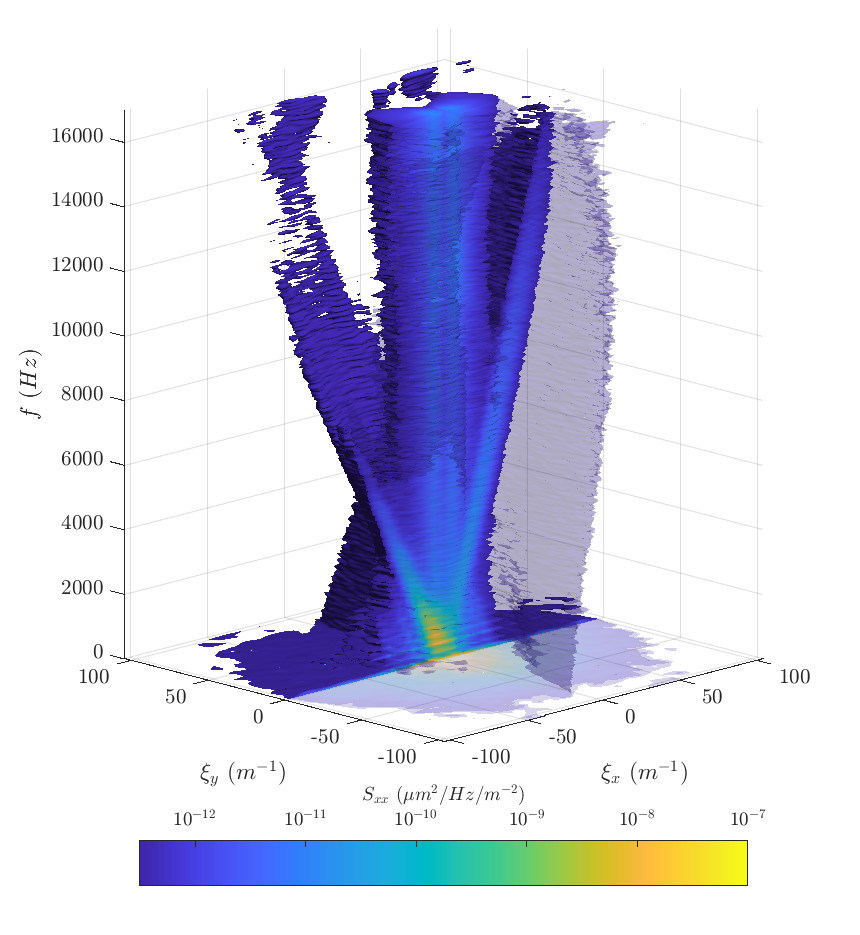
\includegraphics{../matlab/05_synthetic_wavefront/dispersion_comp_real.eps}
  \caption{Multidimensional spectral estimation that the synthetic wavefront is based.}
  \label{fig:05_dispersion_comp_real}
\end{figure}
The optical wavefront was measured in the University of Notre Dame Whitefield wind tunnel at a Mach number of 0.6 with a 10-inch diameter beam.
The beam angle through the test section was $90^\circ$.

The signals that were assumed to be statistically independent from one another, such as the boundary layer signal, were converted into dimensional space separately and then summed together, while signals that were assumed to be related to one another, such as the sound and vibration components, were first summed together in frequency space.
Figure \ref{fig:05_synthetic_dispersion_input} shows the input dispersion plot with each signal component separately colored.
\begin{figure}
 \centering
 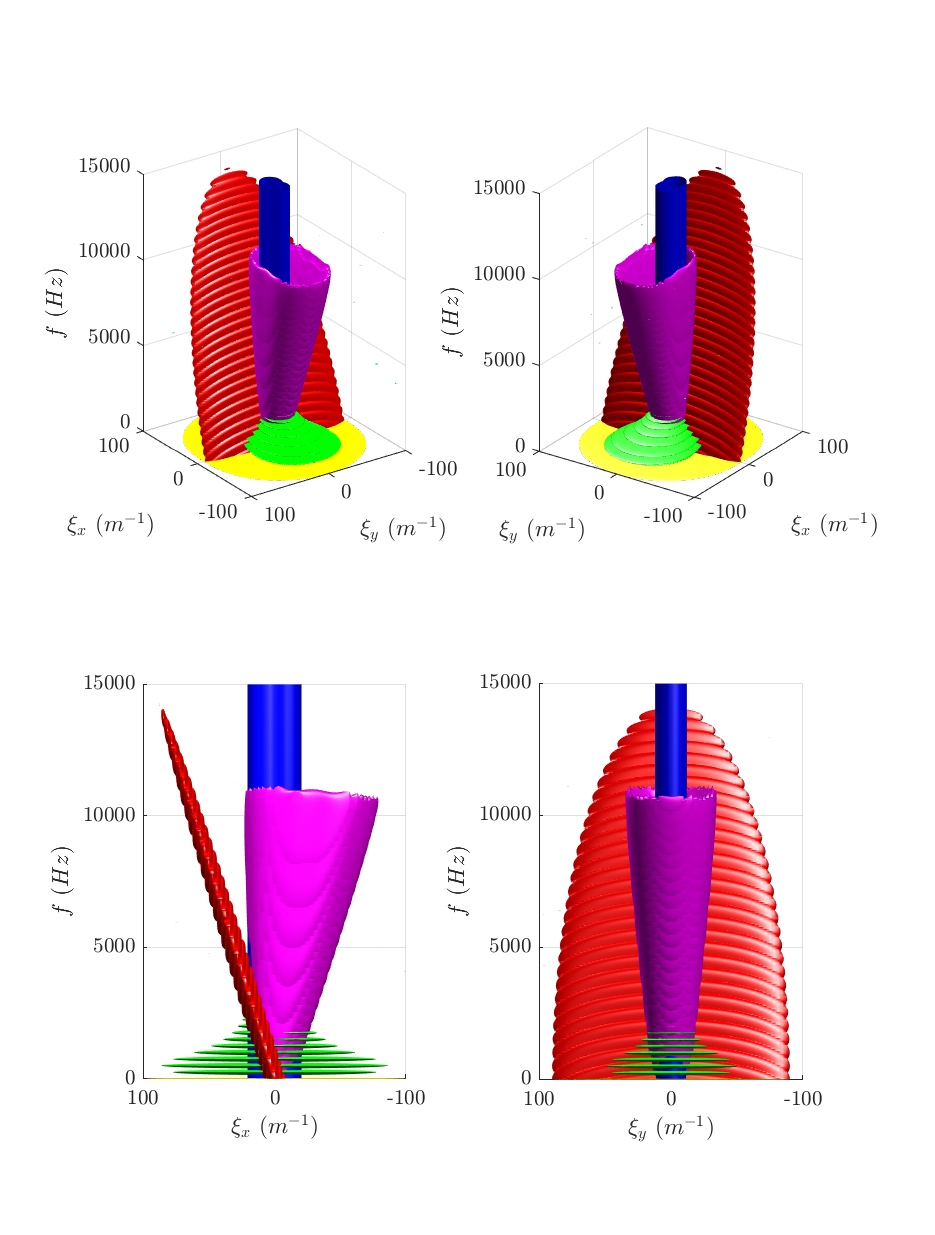
\includegraphics{../matlab/05_synthetic_wavefront/synthetic_wavefront.eps}
 \caption{Synthetic wavefront input dispersion plot of an aero-optical signal and various signal corruption components.  The aero-optical signal is shown in red, the stationary modes in blue, duct acoustics in magenta, blade-passing frequency related corruption in green, slowly varying mean-lensing in yellow, and background in cyan.}
 \label{fig:05_synthetic_dispersion_input}
\end{figure}
The aero-optical signal is shown in red, the stationary modes in blue, duct acoustics in magenta, blade-passing frequency related noise in green, slowly varying mean-lensing in yellow, and background noise in cyan.

\section{General Spectrum Construction}
The general process of developing most of the component signals was to determine an approximate shape, normalize it in the appropriate dimensions, and scale the result by using a function derived from a hyperbola,
\begin{equation}
 \frac{\log_{10}(WF)-b}{b^2}-\frac{\xi_{\rho_N}^2}{a^2} = 1 \textrm{,}
 \label{eqn:05_scaling_hyperbola}
\end{equation}
such that the signal strength at unity of the normalized radial frequency, $\log_{10}(WF(\xi_{\rho_N}=1))$, and the limiting slope, $a/b$, are inputs.
This results in the signal strength of the wavefront being
\begin{equation}
 \log_{10}(WF) = b-\sqrt{\frac{\xi_{\rho_N}^2}{m^2}+b^2} \textrm{,}
 \label{eqn:05_wavefront_strength}
\end{equation}
where
\begin{equation}
 b = \frac{1}{2\log_{10}(WF(\xi_{\rho_N}=1))}\cdot\left(\log_{10}(WF(\xi_{\rho_N}=1))^2-\frac{1}{m^2}\right) \textrm{.}
 \label{eqn:05_wavefront_strength_b}
\end{equation}
The code used to generate the synthetic wavefront used in this section is shown in Appendix \ref{code:sc_synthetic_wavefront}.

\section{Aero-Optical Signal}
The aero-optical signal was generated to approximate an optical beam passing perpendicularly through a test section with boundary layers on each of the test section walls.
An ellipsoid was chosen to approximate the boundary-layer signal because it is the simplest shape that best resembles the aero-optical signal in Figure \ref{fig:05_dispersion_comp_real}.
This signal was approximated by creating an ellipsoid,
\begin{equation}
  \xi_{\rho_N}^2 = (\xi_{x,R}/a_x)^2+(\xi_{y,R}/a_y)^2+(f_R/a_t)^2
\end{equation}
which had been rotated into the plane representing the boundary-layer's dispersion velocity,
\begin{equation}
  \left[\begin{array}{c} \xi_{x,R} \\ \xi_{y,R} \\ f_R \end{array}\right] = \left[\begin{array}{c c c} \cos\theta_u & 0 & \sin\theta_u \\ 0 & 1 & 0 \\ -\sin\theta_u & 0 & \cos\theta_u \end{array}\right]\left[\begin{array}{c} \xi_{x} \\ \xi_{y} \\ f \end{array}\right]
\end{equation}
where $\theta_u=\tan^{-1}(-1/u_{BL})$.
Equations \ref{eqn:05_wavefront_strength} and \ref{eqn:05_wavefront_strength_b} were then used to calculate the multidimensional spectrum of the boundary layer signal.
% The code used to generate the multidimensional spectrum of the boundary layer signal are shown in lines 18-31 of Appendix \ref{code:sc_synthetic_wavefront} and
The values used are shown in Table \ref{tab:05_boundary_layer}.
In Figure \ref{fig:05_synthetic_dispersion_input} the aero-optical signal is shown in red.
\begin{table}
  \centering
  \caption{Values used in the construction of the multidimensional spectrum for the boundary layer signal}
  \begin{tabular}{c c}
    Variable & Value \\
    \hline \hline
    $a_x$ & 8 \\
    $a_y$ & 90 \\
    $a_t$ & 175 \\
    $m$ & -0.13 \\
    $u_{BL}$ & 163.2 m/s \\
    $\log_{10}(WF(\xi_{\rho_N}=1))$ & -14.5
  \end{tabular}
  \label{tab:05_boundary_layer}
\end{table}

\section{Stationary Mode Signals}
The collection of stationary modes is a temporally constant signal at low spatial frequencies that is often has a cross-section in the plane of spatial-frequencies that is circular.
In the particular case that is being modeled, the stationary modes have a cross-section of two circular regions offset along the $\xi_x$-axis that just overlap one another.
A smooth function was chosen to approximate this overlapping circle type stationary mode,
\begin{equation}
 \xi_{\rho_N} = \frac{\xi_\rho}{\xi_{\rho_0}\sqrt{10-6\cos{(2\xi_\theta+\pi)}}} \textrm{.}
 \label{eqn:05_epicycloid_simple}
\end{equation}
This spectrum for the stationary modes component is shown in blue in Figure \ref{fig:05_synthetic_dispersion_input}.
 % and the relevant code shown in Lines 33-40 of Appendix \ref{code:sc_synthetic_wavefront}.
Table \ref{tab:05_stationary_modes} shows the values used in generating the spectrum.
\begin{table}
  \centering
  \caption{Values used in the construction of the multidimensional spectrum for the signal of the stationary modes}
  \begin{tabular}{c c}
    Variable & Value \\
    \hline \hline
    $m$ & -0.175 \\
    $\xi_{\rho_0}$ & 5 \\
    $\log_{10}(WF(\xi_{\rho_N}=1))$ & -14.5
  \end{tabular}
  \label{tab:05_stationary_modes}
\end{table}

\section{Sound and Vibration Signals}
The sound and vibrating component signals are comprised of two parts.
The first of these is the blade-passing frequency and its harmonic disturbances (shown in green in Figure \ref{fig:05_synthetic_dispersion_input}) and the second is the acoustic duct modes (shown in magenta).

\subsection{Blade-Passing Frequency Disturbance}
Like the stationary modes, the blade-passing frequency disturbances were modeled with the same cross-sectional shape as the stationary mode, Equation \ref{eqn:05_epicycloid_simple}, but as narrow-band discs,
\begin{equation}
  \xi_{\rho_N}^2 = \frac{\sqrt{\xi_x^2+(AR\xi_y)^2}}{\xi_{\rho,BPF}\sqrt{10-6\cos(2\xi_\theta+\pi)}}+\left(\frac{f\pm BPF n}{f_T}\right)^2
  \label{eqn:05_blade_passing_frequency}
\end{equation}
where $AR$ is the aspect ratio of the cross-sectional shape, $n$ is the harmonic number, $f_T$ is the disc thickness, and $\xi_{rho,BPF}$ is
\begin{equation}
  \xi_{rho,BPF} = \frac{\xi_{\rho_0}}{\sqrt{1+\frac{BPF n-BPF}{f_c}}}
\end{equation}
where $f_c$ is the effectively cutoff frequency for modulating the strength of each disc as the harmonic number increased from $n=0.5$ to $n=5$ in steps of 0.5.
% The code for the blade-passing frequency disturbances is shown in Lines 42-60 of Appendix \ref{code:sc_synthetic_wavefront} with
A list of values is shown in Table \ref{tab:05_bpf}.
\begin{table}
  \centering
  \caption{Values used in the construction of the multidimensional spectrum for the blade-passing frequency disturbance}
  \begin{tabular}{c c}
    Variable & Value \\
    \hline \hline
    $AR$ & 1 \\
    $BPF$ & 500 Hz \\
    $f_c$ & 500 Hz \\
    $f_T$ & 100 Hz \\
    $m$ & -0.13 \\
    $\xi_{\rho_0}$ & 20 \\
    $\log_{10}(WF(\xi_{\rho_N}=1))$ & -14
  \end{tabular}
  \label{tab:05_bpf}
\end{table}


\subsection{Acoustic Cone}
The acoustic duct mode disturbances form a cone which in the $f-\xi_x$ plane is defined by the lines $u\pm c$, while in the $f-\xi_y$ plane is defined by the speed of sound.
At each temporal frequency step an ellipse was defined based on the constraining lines and the distance to that ellipse used to calculate a normalized radial frequency,
\begin{equation}
  \xi_{\rho_N}^2 = \frac{\sqrt{(\xi_x-\xi_{x_0})^2+(\xi_y-\xi_{y_0})^2}}{\sqrt{\xi^2_{x_a}\cos^2\xi_\theta+\xi^2_{y_a}\sin^2\xi_\theta-1}} \frac{\sqrt{\xi^2_{x_a}\cos^2\xi_\theta+\xi^2_{y_a}\sin^2\xi_\theta}}{\xi_{\rho_T}} \textrm{,}
\end{equation}
where $\xi_{x_0}$ and $\xi_{y_0}$ are the midpoint between the sonic lines in the x and y directions as a function of $f$, $\xi_{x_a}$ and $\xi_{y_a}$ are the distances from the midpoint to the sonic lines as a function of $f$, and $\xi_{\rho_T}$ is the thickness of the ellipse.
The strength of the disturbance was decreased logarithmically as a function of $|f|$ from $f=0$ to $f=f_s/2$ with Equation \ref{eqn:05_wavefront_strength_b} becoming,
\begin{equation}
  b(f) = \frac{1}{2b_0(f)}\left(b_0^2(f)-\frac{1}{m^2}\right) \textrm{,}
\end{equation}
where
\begin{equation}
  \begin{aligned}
    b_0(f) =& \frac{\log_{10}(WF(\xi_{\rho_N}=1,f=f_s/2))-\log_{10}(WF(\xi_{\rho_N}=1,f=0))}{f_s/2}|f| \\ &+\log_{10}(WF(\xi_{\rho_N}=1,f=f_0)) \textrm{.}
  \end{aligned}
\end{equation}

Two low-pass spatial filters (more discussion in Chapter \ref{chap:06_single_filter}) were used to replicate some of the signal attenuation that happens at the low spatial frequencies in the x-direction.
First a low-pass filter in $\rho$ was used,
\begin{equation}
  WF = WF\sqrt{\frac{1}{1+\left(\frac{\xi_\rho}{\xi_{c_\rho}}\right)^2}} \textrm{,}
\end{equation}
followed by a low-pass filter in the x-direction,
\begin{equation}
  WF = WF\sqrt{\frac{1}{1+\left(\frac{\xi_x}{\xi_{c_x}}\right)^2}} \textrm{.}
\end{equation}
The values used in creating the spectrum are shown in Table \ref{tab:05_cone}.
 % and the code is shown in lines 74-93 of Appendix \ref{code:sc_synthetic_wavefront}.
\begin{table}
  \centering
  \caption{Values used in the construction of the multidimensional spectrum for the acoustic cone disturbance}
  \begin{tabular}{c c}
    Variable & Value \\
    \hline \hline
    $m$ & -0.3 \\
    $\xi_{c_x}$ & 115 m$^{-1}$ \\
    $\xi_{c_\rho}$ & 200 m$^{-1}$ \\
    $\xi_{\rho_T}$ & 8 m$^{-1}$ \\
    $\log_{10}(WF(\xi_{\rho_N}=1,f=0))$ & -13 \\
    $\log_{10}(WF(\xi_{\rho_N}=1,f=f_s/2))$ & -16
  \end{tabular}
  \label{tab:05_cone}
\end{table}

\section{Mean-Lensing Signal}
The mean lensing part of the optical signal is the integrated effect of steady optical aberrations added by lenses, mirror, windows, etc, in the beam path.
The aberrations are effectively random and a physical model cannot be developed for them.
The mean-lensing signal (shown in yellow in Figure \ref{fig:05_synthetic_dispersion_input}) uses same cross-sectional as the blade-passing frequency disturbances and represents the slowly varying spatial disturbance,
\begin{equation}
  \xi_{\rho_N}^2 = \frac{\sqrt{\xi_x^2+(AR\xi_y)^2}}{\xi_{\rho_0}\sqrt{10-6\cos(2\xi_\theta+\pi)}}+\left(\frac{f}{f_T}\right)^2 \textrm{.}
  \label{eqn:05_mean_lensing}
\end{equation}
% The relevant code is shown on lines 62-72 of Appendix \ref{code:sc_synthetic_wavefront} with values shown in Table \ref{tab:05_mean_lensing}.
Table \ref{tab:05_mean_lensing} shows a list of the values used in creating this component of the wavefront signal.
\begin{table}
  \centering
  \caption{Values used in the construction of the multidimensional spectrum for the mean-lensing disturbance}
  \begin{tabular}{c c}
    Variable & Value \\
    \hline \hline
    $AR$ & 0.55 \\
    $f_T$ & 50 Hz \\
    $m$ & -0.5 \\
    $\xi_{\rho_0}$ & 25 \\
    $\log_{10}(WF(\xi_{\rho_N}=1))$ & -14.5
  \end{tabular}
  \label{tab:05_mean_lensing}
\end{table}

\section{Background Noise Signal}
Background noise in the wavefront data originates from sources which are random in nature.
The background noise disturbance (with a few small spots shown in cyan in Figure \ref{fig:05_synthetic_dispersion_input}) was simulated using normally distributed random noise with a mean noise level, $\mu(\log_{10}(WF))=-18$, and deviation, $\sigma(\log_{10}(WF))=0.75$.
% The relevant code is shown in lines 95-100 of Appendix \ref{code:sc_synthetic_wavefront}.

\section{Synthetic Wavefront Creation}
A synthetic signal can be created from a power spectrum by solving for $x$ in Equation \ref{eqn:04_basic_sxx} and using the Inverse Fast Fourier Transform,
\begin{equation}
 x(t) = \real\left[\ifft\left\{\sqrt{S_{xx}\cdot N\cdot f_{samp}}\cdot\exp{i\phi}\right\}\right] \textrm{,}
 \label{eqn:05_ifft}
\end{equation}
where $\real$ is the real component and $\phi$ is a random set of phases for each point in the measurement space.
As shown previously this relation can be extended into $n$-dimensions,
\begin{equation}
 f(\mathbf{x}) = \real\left[\ifftn\left\{\sqrt{\mathbf{S_{xx}}\cdot\prod{\overrightarrow{N}\cdot \overrightarrow{f}_{samp}}}\cdot\exp{i\mathbf{\phi}}\right\}\right] \textrm{.}
 \label{eqn:05_ifftn}
\end{equation}
Care should be taken when constructing the random set of phases, as the zero-frequency component has zero phase, $\phi(0,0,0) = 0$, and the phases on either side of it are conjugates of one another, $\phi(\pm\xi_x,\pm\xi_y,\pm f)=-\phi(\mp\xi_x,\mp\xi_y,\mp f)$.
% The code for creating a wavefront from a multidimensional spectrum is shown in lines 196-202 of Appendix \ref{code:sc_synthetic_wavefront} and is specifically creating the wavefront for the aero-optical signal but other signals are generated using the same basic code.
% Note that the first three lines are to get the set of phases properly configured that creates conjugate phases rotated about the origin.

It was assumed that the aero-optical signal, the stationary modes, the background noise, and the sound and vibration combination of modes were statistically independent of one another and, as such, could be separately transformed into physical space.
The components of the sound and vibration sources, the blade-passing frequency, the acoustic cone, and the mean-lensing, were assumed to be related to one another and thus were summed together in frequency space prior to being transformed into physical space.
Once the separate components were in physical space the total wavefront was obtained by summing up the separate components with the aero-optical signal saved along side the total wavefront.
Some frames from the synthetic wavefront are shown in Figure \ref{fig:05_synthetic_frames} with the total wavefront shown on top and the aero-optical only signal shown on the bottom.
\begin{figure}
 \centering
 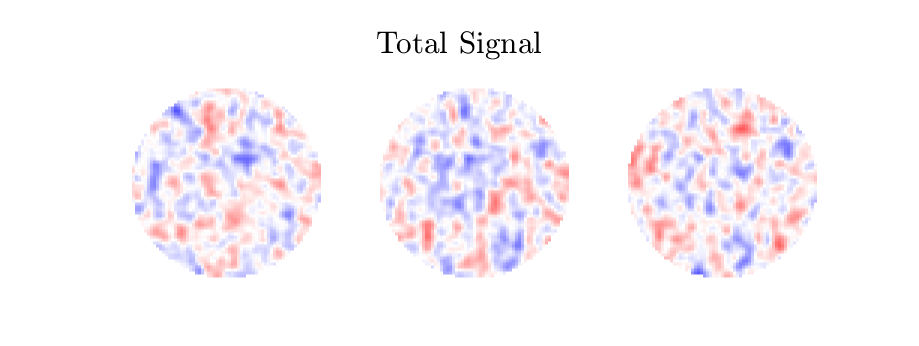
\includegraphics{../matlab/05_synthetic_wavefront/synthetic_frames_total.eps}
 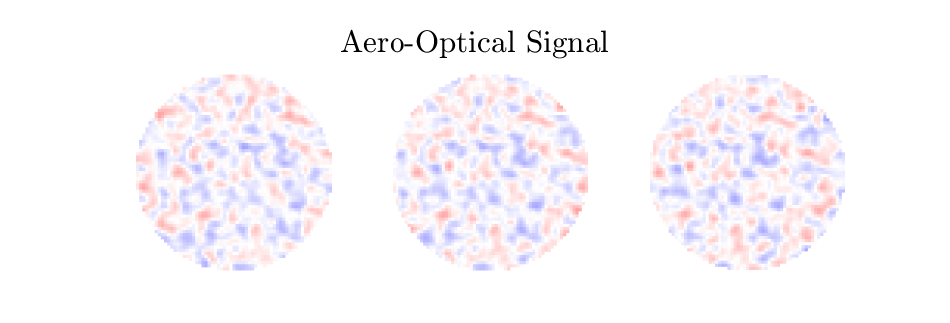
\includegraphics{../matlab/05_synthetic_wavefront/synthetic_frames_ao.eps}
 \caption{Sample frames from the synthetic wavefront with the total wavefront signal on top and the aero-optical only signal bottom.  Flow is from right to left.}
 \label{fig:05_synthetic_frames}
\end{figure}
Flow is from right to left.
The aero-optical signal is noticeable to some degree in the total wavefront signal, but can be overpowered by the various noise sources.

\section{Comparison to Measured Data}
A multidimensional spectral plot of the total synthetic wavefront is shown in Figure \ref{fig:dispersion_comp_synthetic}.
\begin{figure}
 \centering
 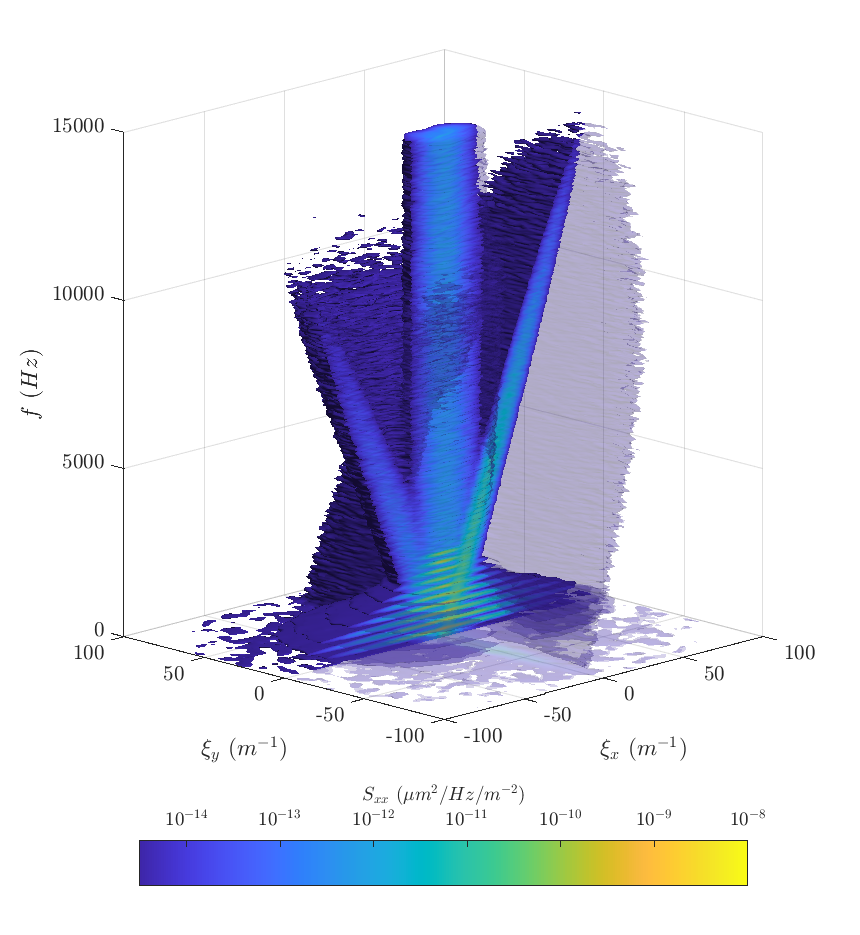
\includegraphics{../matlab/05_synthetic_wavefront/dispersion_comp_synthetic.eps}
 \caption{Synthetic wavefront output dispersion plot of an aero-optical signal and various signal corruption components.}
 \label{fig:dispersion_comp_synthetic}
\end{figure}
In this view the aero-optical signal is more noticeable but there still remains some significant overlap with the various noise sources.
While the mean-lensing component is not as visible in this isosurface, the rest of the dispersion plot in a good representation of the input dispersion plot shown in Figure \ref{fig:05_synthetic_dispersion_input}.
The blade-passing frequency was depicted as symmetric in the synthetic wavefront while measured data (shown in Figure \ref{fig:04_dispersion_3d}) shows more signal on the side traveling in the direction of flow.
The harmonics of the BPF are more on the upstream traveling side of the dispersion and are a little less pronounced in the measured data.
The total synthetic wavefront has a $\opdrms$ of $0.0112\pm0.0006\mu m$ with the aero-optical only signal having a $\opdrms$ of $0.0073\pm0.0003\mu m$.
The measured wavefront presented in Figure \ref{fig:04_dispersion_3d} had a $\opdrms$ of $0.0874\pm0.0263\mu m$.
The overall $\opdrms$ of the synthetic wavefront was $12.8\%$ when compared to the measured wavefront indicating that the algorithms used to generate the wavefront are not representative of reality and can provide a future path of research in order to produce more realistic synthetic wavefronts.

    % !TEX root = catron-dissertation.tex
\epstopdfsetup{outdir=./images/06_single_sensor_filtering/}

\chapter{Wavefront Multidimensional Spectral Filtering Techniques}
\label{chap:06_single_filter}
% \textcolor{red}{
%   \begin{itemize}
%     \item Work on the chapter intro
%     \item Filter applied in Fourier space and multidimensional spectral space
%   \end{itemize}
% }

This chapter will examine a variety of filtering techniques used on multidimensional spectra of optical wavefronts.
While none of the filters presented here are novel, many are based on well known digital filters, their application to filtering optical wavefronts is something that needs to be studied.
This chapter will start out by examining some filters that are applied to just the wavefront data itself and will then examine a filtering technique that incorporates additional sensors data in the filtering process.

By using multidimensional spectral estimates on wavefronts, as shown in Chapter \ref{chap:04_dispersion}, differences in source disturbances become clearly evident.
When just the wavefront measurement itself is available, digital filters can be used to separate or isolate a single disturbance source or at least minimize the impact from other sources.
The digital filters used in this dissertation, use a transfer function, $H(j\omega)$, and are applied in Fourier space.
The transfer functions themselves are typically derived in Laplace space, $H(s)$, but because $s=j\omega$ they are valid in Fourier space as well \cite{Hamming-1998-CdhcDuvZ}.
The transfer function is composed of two components which attenuate the signal, gain and phase.
The filter gain is the magnitude of the transfer function, $G(\omega) = |H(j\omega)|$, while the filter phase is the argument, $\Phi(\omega) = \arg(H(j\omega))$.
In the simplest case, the filtered signal is the inverse Fourier transform of the gain multiplied by the Fourier transform of the signal,
\begin{equation}
 f_F(\mathbf{x}) = \real\left(\ifftn[H(j\mathbf{\omega})\fftn\{\mathbf{x}\}]\right) \textrm{,}
 \label{eqn:06_filter_function}
\end{equation}
where $f$ is the signal function and $f_F$ is the filtered signal.

\section{Temporal Filter Methods}
The methods presented in this section are based on Butterworth filters but could be extended to other types of filters.
The square of the transfer function of a Butterworth filter is \cite{Butterworth-1930-DvDrjKha},
\begin{equation}
 |H(j\omega)|^2 = G^2(\omega) = \frac{G_0^2}{1+\left(\frac{j\omega}{j\omega_c}\right)^{\pm2n}} \textrm{,}
 \label{eqn:06_butterworth}
\end{equation}
where $G_0$ is the zero-frequency gain, $\omega_c$ is the cutoff angular frequency, $n$ is the filter order (number of filters in a series), and $\pm$ represents either a low-pass ($+$) or high-pass ($-$) filter.
The gain of this filter is
\begin{equation}
  G(\omega) = \frac{G_0}{\sqrt{1+\left(\frac{\omega}{\omega_c}\right)^{\pm2n}}} \textrm{.}
  \label{eqn:06_butterworth_gain}
\end{equation}
A band-pass filter can be constructed by placing a low-pass filter in series with a high-pass filter and a band-stop by placing the two types in parallel.

In many tests, a large portion of the wavefront noise is at low frequencies primarily caused by mechanical vibration.
In general, a high-pass filter is useful in temporal space for removing this noise, since in many cases most of the power in the aero-optical signal occurs at higher frequency than the low-frequency mechanical vibration. as shown in Figure \ref{fig:06_filter_temporal}.
\begin{figure}
 \centering
 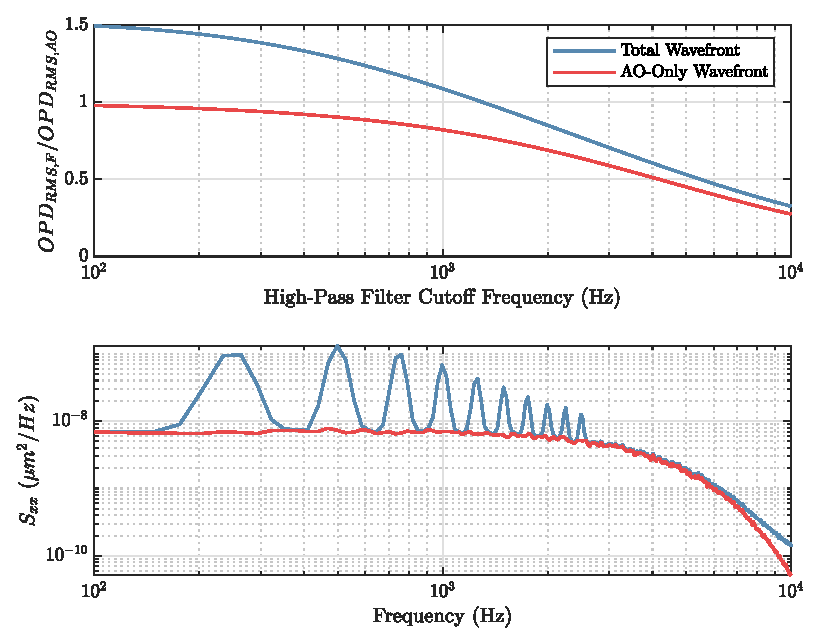
\includegraphics{../matlab/06_single_sensor_filtering/filter_temporal.eps}
 \caption{The $opdrms$ of high-pass temporal filtered wavefronts relative to the $opdrms$ of the aero-optical only unfiltered wavefront (top). Power spectra of both of the simulated wavefront versions (bottom).}
 \label{fig:06_filter_temporal}
\end{figure}
The top plot in this figure shows the high-pass filtered $\opdrms$ of both the total and aero-optical only wavefronts normalized by the unfiltered $\opdrms$ of the aero-optical only wavefront, for high-pass filters with various cutoff frequencies.
The results in Figure \ref{fig:06_filter_temporal} were computed using wavefronts that were simulated using the methods described in Chapter \ref{chap:05_synthetic}.
For reference, the bottom plot of Figure \ref{fig:06_filter_temporal} shows the power spectra of just the aero-optical portion of the wavefront (red curve) and the total wavefront (blue curve) which includes vibration-related peaks associated with the blade-passing frequency and its harmonics.
The figure shows how a high-pass filter decreases the energy in the total wavefront and in the actual aero-optical wavefront, as the filter cutoff frequency increases.
As shown in the top plot, at low cutoff frequency, the filter primarily removes vibration effects from the total signal; however, as the cutoff frequency increases, the filter also removes actual aero-optical signal.
Around 1,200 Hz, the $\opdrms$ of the total signal is equal to the $\opdrms$ of the actual aero-optical signal; at this cutoff frequency ~75\% of the aero-optical signal remains and the remaining signal is made up by the remaining contamination.
This approach can provide a computationally inexpensive way of estimating the aero-optical portion of the wavefront for calculations that rely on the $\opdrms$ of a wavefront.
While it is more straightforward to determine a cutoff frequency for this synthetic wavefront since all of the signal components are fully known, a measured wavefront will likely take some knowledge or expectation of the contamination that is present in the measurement in order to select a high-pass filter cutoff frequency.

% \ref{tab:test}
% \begin{table}
% \centering
% \caption{Test Table}
% \input{../matlab/04_basic_filtering/filter_temporal.txt}
% \label{tab:test}
% \end{table}

An example of wavefronts that result from band-pass and band-stop filtering is shown in Figure \ref{fig:06_filter_temporal_bandpass}.
\begin{figure}
 \centering
 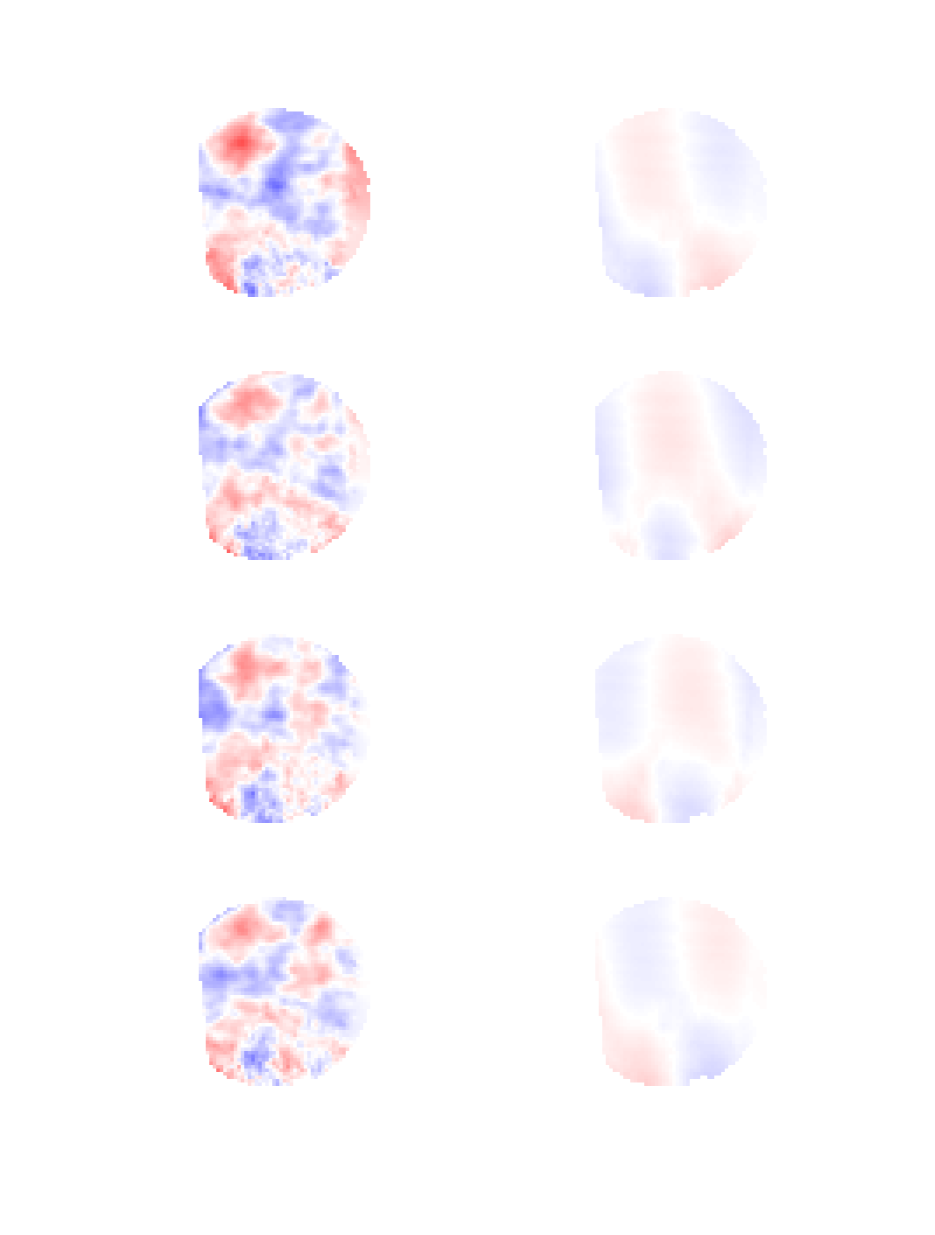
\includegraphics{../matlab/06_single_sensor_filtering/filter_temporal_bandpass.eps}
 \caption{Measured wavefronts filtered at the blade-passing frequency (532$\pm$10 Hz).  The left column is band-stop filtered while the right is band-pass filtered.}
 \label{fig:06_filter_temporal_bandpass}
\end{figure}
The figure shows several wavefront frames of measured data acquired in the Notre Dame White Field wind tunnel and presented previously in Chapter \ref{chap:03_optical_acoustics} (see Figure \ref{fig:03_tunnel_comparison}) that are band-stop filtered in the left column and band-pass filtered in the right column.
The flow is from right-to-left and the band-pass filtered wavefront clearly shows upstream-moving optical disturbances (moving left-to-right against the flow direction) associated with acoustic duct modes traveling upstream from the fan.
On the other hand, the band-stop filtered wavefronts on the left of Figure \ref{fig:06_filter_temporal_bandpass} show much slower-moving optical disturbances that are in general moving in the direction of the flow.
In particular, the downstream-moving disturbances on the left side of Figure \ref{fig:06_filter_temporal_bandpass} have the appearance of boundary-layer aero-optical disturbances, with a scale on the order of the boundary-layer thickness.

Note that for filters that operate in one dimension, the filters were applied over both positive and negative frequencies to the n-dimensional Fourier transform in order to preserve the direction of travel of the signal.
This also allowed several filters to be applied in series without having to perform a Fourier and inverse Fourier transform for each successive filter.
Temporal filters are also used in sizing and/or designing adaptive optics systems \cite{Greenwood-1977-aWDqUh6C} for example.
A low-pass filter with a cutoff at the bandwidth of either a fast-steering or deformable mirror is often used to define the signal that the system needs to reject \cite{Whiteley-2007-bHbWRWUu}.
A control system may need to have the bandwidth reduced in order to keep a mirror’s travel within limits \cite{Madec-2012-YJ8eWhPB}, while a high-pass filter would inform designers of the remaining optical aberrations that cannot be corrected.

\section{Upstream/Downstream Moving}
\label{chap:06_up_down_filter}
In the preceding section, filters based on temporal frequency only were discussed. In this section, another filtering approach is presented in which signals are identified based on their dispersion velocity.
For the filtering of upstream and downstream moving optical disturbances a logistic function was chosen,
\begin{equation}
 f(x) = \frac{1}{1+\exp\{-kx\}} \textrm{.}
 \label{eqn:06_logistic}
\end{equation}
This function was then expanded into two-dimensions ($x$ and $t$).
For a filter that removes disturbances moving against the direction of flow, the filter should ideally return a value of one in both the first and third quadrants and zero otherwise when plotted in a graph of temporal versus spatial frequency.
To accomplish this, the logistic curve in each dimension was scaled and offset to output values between negative one and positive one,
\begin{equation}
 G_t(f) = \frac{2}{1+\exp\{-k_tf\}}-1
 \label{eqn:06_logistic_time}
\end{equation}
and
\begin{equation}
 G_x(\xi_x) = \frac{2}{1+\exp\{\pm k_x\xi_x\}}-1 \textrm{,}
 \label{eqn:06_logistic_space}
\end{equation}
where $\pm$ determines whether the filter is designed to act on upstream-traveling disturbances ($+$) or downstream-traveling ($-$).
These two gain functions are then multiplied together and scaled to output values between zero and one,
\begin{equation}
 G(\xi_x,f) = \frac{(G_t\cdot G_x)+1}{2} \textrm{.}
 \label{eqn:06_up_down_filter}
\end{equation}
As the values of $k_x$ and $k_t$ go to infinity an ideal filter is obtained.
In a plot of the gain with the horizontal spatial frequency on the x-axis and the temporal frequency on the y-axis, an ideal filter for obtaining only the downstream traveling disturbances would have a gain of one in the first and third quadrants, zero in the second and fourth quadrants, and a value of $1/2$ when either frequency is zero.
The value of $1/2$ would equally split the component of a disturbance that is neither traveling upstream or downstream between the two directions.

The multidimensional spectrum using an ideal upstream-moving filter on the synthetic wavefront is shown in Figure \ref{fig:06_filter_downstream} alongside the spectrum of the unfiltered wavefront.
\begin{figure}
 \centering
 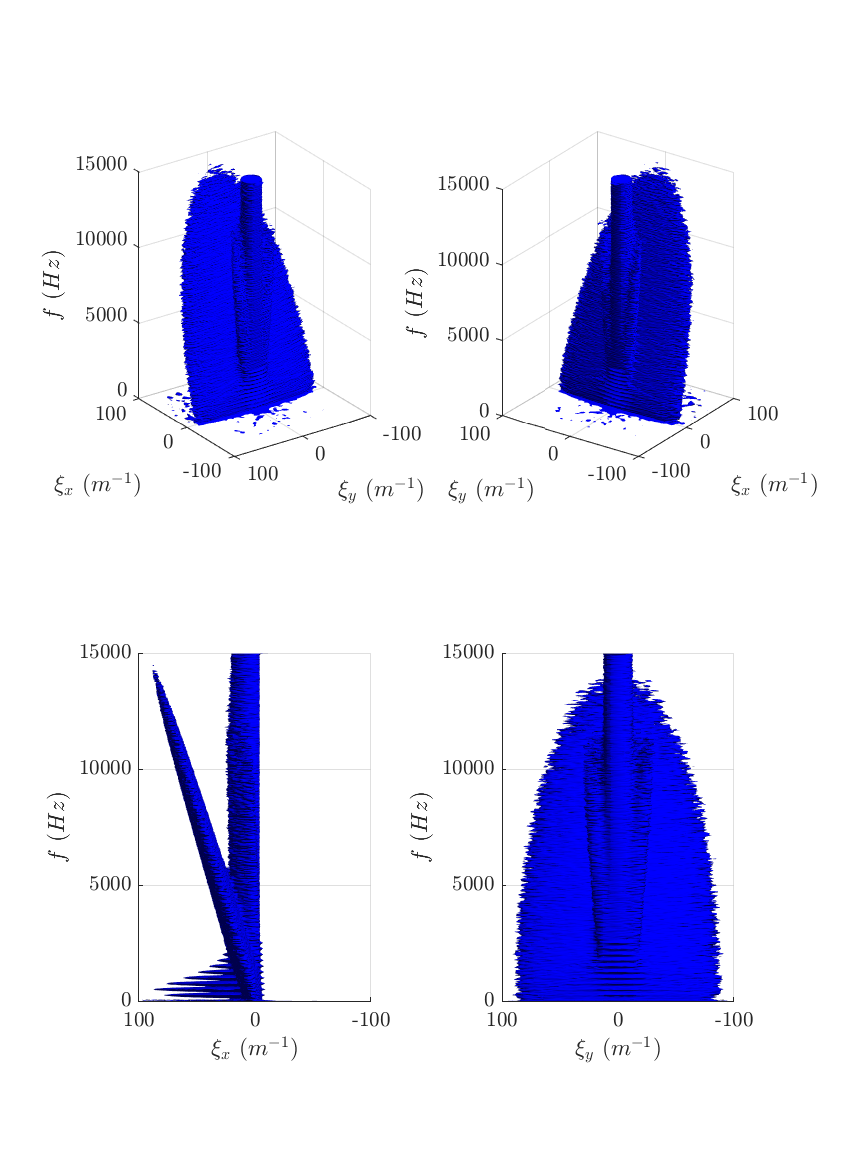
\includegraphics{../matlab/06_single_sensor_filtering/filter_downstream.eps}
 \caption{Multidimensional spectral isosurface of the synthetic wavefront with a downstream filter in place.}
 \label{fig:06_filter_downstream}
\end{figure}
All of the upstream traveling disturbances are removed and the disturbances at the stream-wise spatial frequency $\xi_x=0$ m$^{-1}$ are significantly reduced.
Some of the stationary modes (the vertical cylinder along $\xi_x=0$ and $\xi_y=0$) remain while only the acoustic and vibration signals that are propagating in the direction of flow remain.
The aero-optical signal from the boundary layer is clipped slightly at $\xi_x=0$ due to the spatial width of the signal.
The ratio of the time-averaged spatial-RMS of the filtered signal when compared to the aero-optical only signal was 1.24 while the unfiltered ratio was 1.53.
When the filter was applied to the wavefront with only the aero-optical boundary layer signal present the $\opdrms$ was reduced to 96\% that of the unfiltered wavefront, showing that the filter does not reduce the energy of aero-optical signals convecting with the flow.
Hence, this filter method will retain any disturbance that is traveling in the direction of flow.
Even with an ideal filter there is some slight attenuation of the aero-optical signal due to signal having some spectral width that crosses into upstream-moving portion of the dispersion plot.


\section{Velocity Filtering}
\label{chap:06_velocity_filter}
For a nondispersive medium such as air, flow structures traveling at a given speed have a constant slope on a multidimensional spectral plot.
A plane in the multidimensional spectral plot can therefore be used to measure a flow structure's velocity in both $x$ and $y$-directions.
The distance from any given point in the multidimensional spectral space to a plane described by the velocities $u_x$ and $u_y$ can be computed by
\begin{equation}
 d = \frac{|u_x\xi_x+u_y\xi_y-f|}{\sqrt{u_x^2+u_y^2+1}} \textrm{.}
 \label{eqn:06_dist_point_2_plane}
\end{equation}
Equation \ref{eqn:06_dist_point_2_plane} above can therefore be used to construct a low-pass or high-pass filter that retains only disturbances that are traveling at that velocity, or to exclude those disturbances,
\begin{equation}
  G(d) = \frac{1}{\sqrt{1+\left(\frac{d}{d_c}\right)^{\pm2n}}} \textrm{.}
  \label{eqn:06_butterworth_velocity}
\end{equation}
where $d_c$ is the cutoff distance from the plane defined by the velocities $u_x$ and $u_y$.
Because of differences in the temporal and spatial sample rates of several orders of magnitude, the filter function employed in this research used frequencies that have been normalized by the sample rate.

An example of a low-pass velocity-filter applied to the synthetic wavefront generated in Chapter \ref{chap:05_synthetic} is shown in Figure \ref{fig:06_filter_velocity}.
\begin{figure}
 \centering
 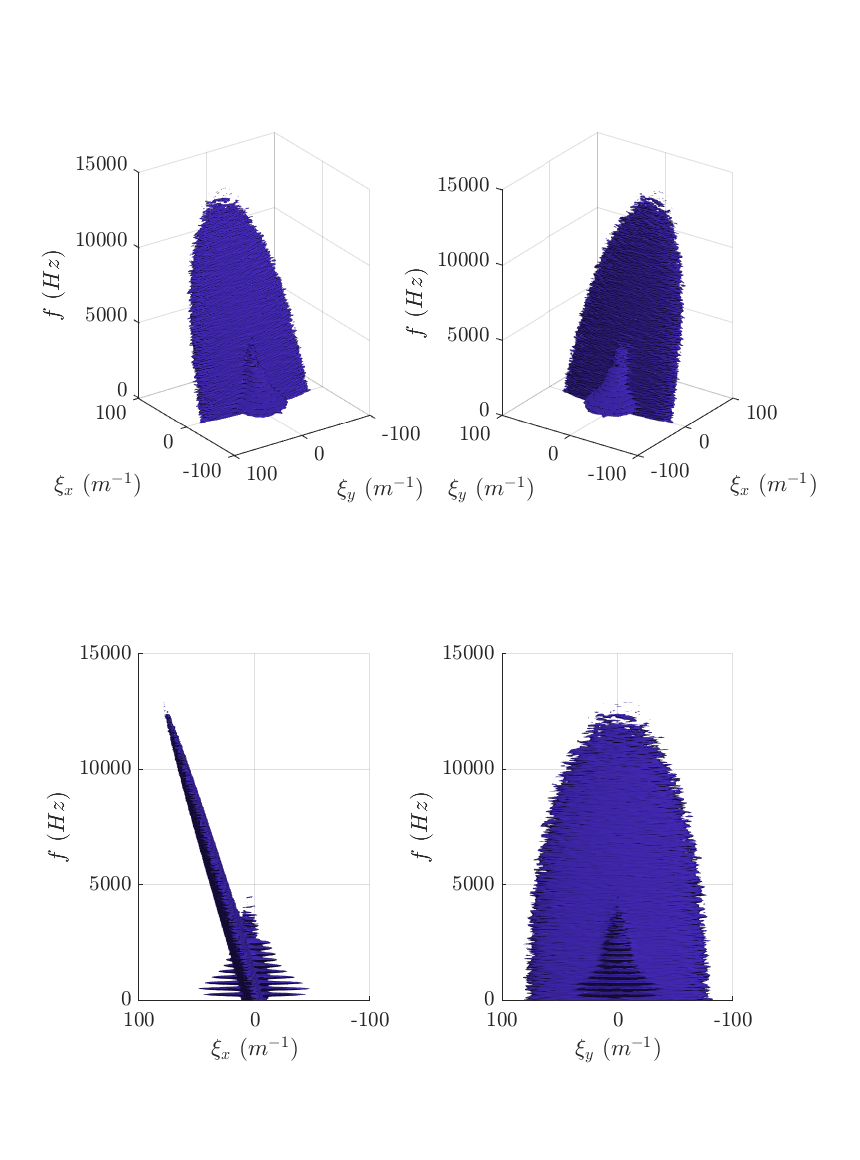
\includegraphics{../matlab/06_single_sensor_filtering/filter_velocity.eps}
 \caption{Multidimensional spectral isosurface of the synthetic wavefront with a low-pass velocity-filter in place.}
 \label{fig:06_filter_velocity}
\end{figure}
The filter was constructed for a $u_x$ set at the mean boundary-layer velocity, and $u_y$ set to zero.
The values of the other two filter parameters were selected as $d_c=1/80$, and $n=1$, which were chosen in a trial-and-error process in which values were chosen, the filtered multidimensional spectrum was computed, and refinements to the parameter values were made based on how well the filtered spectrum captured just the boundary-layer signal.
Figure \ref{fig:06_filter_velocity} shows that, using these filter parameters, the  velocity-filtered multidimensional spectrum successfully retains primarily only the aero-optical signal with some additional low-frequency content from the blade-passing frequency and harmonic disturbances as well as some stationary and acoustic disturbances.
The ratio of the $\opdrms$ relative to that of the aero-optical-only signal went from 1.53 in the unfiltered case to 1.01 in the filtered case, showing that the velocity filter has filtered out a substantial amount of noise and other unrelated signals from the aero-optical signal of the boundary layer, which is presumed to be the objective of the measurement.
As such, this method can provide a very effective way to quickly estimate the $\opdrms$ of a convecting aero-optical disturbance in a noise-contaminated wavefront.

Another use of the velocity filter is measuring the speed of a broadband convecting disturbance such as the aero-optical signal of a boundary layer.
This can be accomplished by applying a series of low-pass velocity filters to the multidimensional spectrum of the wavefront along with a high-pass radial frequency filter to remove a significant portion of the stationary modes and acoustic cone,
\begin{equation}
  S_{xx,f}(\xi_x,\xi_y,f) = S_{xx}(\xi_x,\xi_y,f) G_v^2 G_\rho^2 \textrm{,}
  \label{eqn:06_velocity_filter_measurement}
\end{equation}
where $G_v$ is the velocity filter and $G_\rho$ is the radial frequency ($\xi_rho^2 = \xi_x^2+\xi_y^2$) filter.
Once the wavefront has been filtered in multidimensional spectral space, the total power remaining in the filtered spectrum can be calculated,
\begin{equation}
  P = \sum (S_{xx,f}\prod{\overrightarrow{f_s}}) \textrm{.}
\end{equation}
The average convective velocity of the structure is then given by the filter parameters that produce the maximum power in the filtered signal.

This velocity finding procedure described in the preceding paragraph was tested on the synthetic wavefront generated in Chapter \ref{chap:05_synthetic}, which had a known boundary-layer mean velocity.
The results of the velocity finding analysis are shown in Figure \ref{fig:06_filter_velocity_measure}, which shows the power in the filtered signal as a function of the $u_x$ parameter using in the velocity filter component of Equation \ref{eqn:06_velocity_filter_measurement}.
\begin{figure}
 \centering
 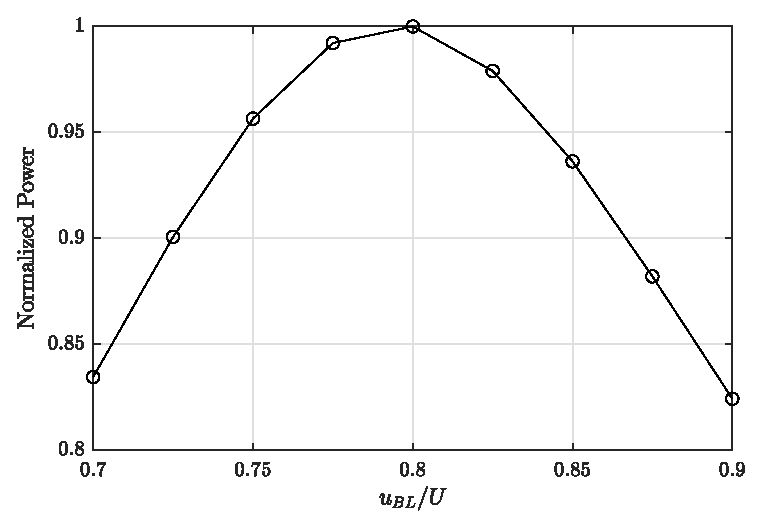
\includegraphics{../matlab/06_single_sensor_filtering/filter_velocity_measure.eps}
 \caption{Boundary layer velocity measurement of the synthetic wavefront using a combination of a low-pass velocity filter and a high-pass radial frequency filter. The maximum value at $u_{BL}/U=0.8$ corresponds with the actual value used in the creation of the synthetic wavefront.}
 \label{fig:06_filter_velocity_measure}
\end{figure}
The low-pass velocity filter used the same parameters as used previously except that $u_x$ was varied and the high-pass radial frequency filter used a cutoff value of 0.1 with an order of $n=2$.
The radial frequency, $\xi_\rho$, was normalized by the spatial sampling rate.
In this case, the boundary layer speed was determined to be 163 m/s which corresponds to the design velocity of the synthetic signal of $0.8U$.
For signals where the mean-velocity component of the aero-optical signal is not aligned with either the horizontal or vertical axis, both velocity components can be varied in the velocity filter.
This produces a three-dimensional surface of filtered signal power as a function of $u_x$ and $u_y$ in the velocity filter, where the velocity components of the moving signal are given by the maximum power of the surface.
An example of this method is shown in Figure \ref{fig:06_filter_velocity_real}, which was computed using experimental wavefront data acquired in the White Field wind tunnel at M=0.5.
\begin{figure}
 \centering
 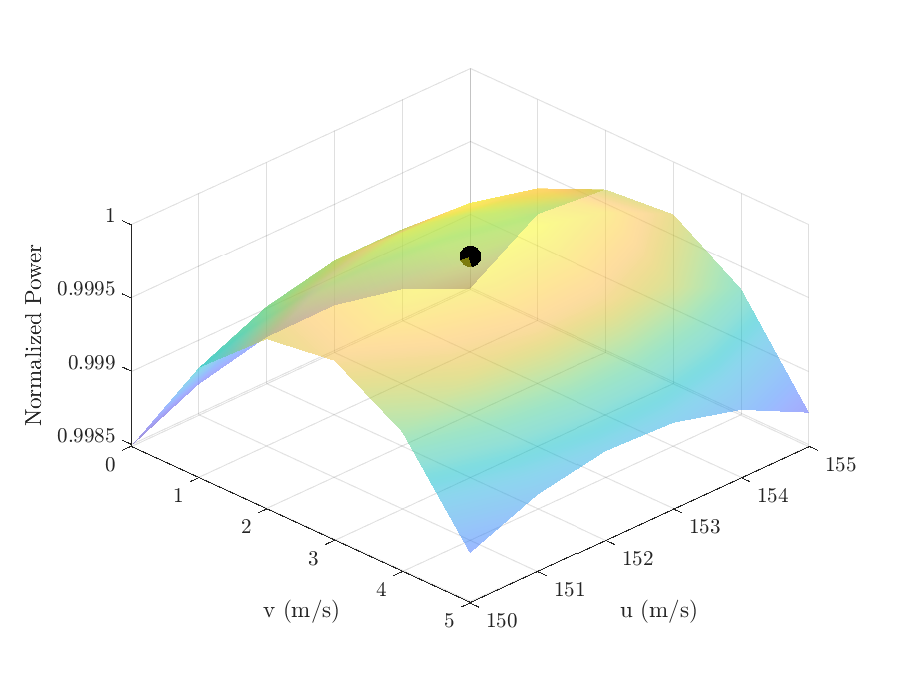
\includegraphics{../matlab/06_single_sensor_filtering/filter_velocity_real.eps}
 \caption{Velocity low-pass filter used to determine the mean disturbance velocity of measured data presented in Figure \ref{fig:04_dispersion_3d}.  The velocity in the x-direction was measured to be 152 m/s and 3 m/s in the y-direction.}
 \label{fig:06_filter_velocity_real}
\end{figure}
In this case the same filtering parameters were used as the synthetic case except the distance cutoff was $d_c=1/40$ and both $u_x$ and $u_y$ were variables.
The velocity components of the boundary-layer optical disturbances determined from Figure \ref{fig:06_filter_velocity_real} are 152 m/s in the x-direction and 3 m/s in the y-direction.
This boundary-layer velocity is approximately 0.85 times the freestream velocity when compared to the pitot probe measurement of the free-stream velocity, which is very close to the accepted speed of the optically-aberrating structures in a boundary-layer flow \cite{Gordeyev-2014-jcJndkHM}.
The overall flow angle of the boundary-layer with respect to the orientation of the measurement beam was approximately $1.1^\circ$.

\section{Baseline Spectrum}
\label{chap:06_baseline}
If all of the narrow-band temporal signals in a data set can be assumed to be measurement contamination that needs to be filtered out, a method for calculating the baseline of the spectrum provides a simple way of filtering a portion of the signal contamination.
For example, during analysis of Raman spectra, the baseline spectra must often be removed \cite{Schulze-2012-GmyAqzC7}.
This task is often performed manually which has resulted in a number of attempts to create automated techniques to estimate the baseline spectra \cite{Mosier-Boss-1995-keK3ckUN, Schulze-2005-QkUeywxD, Schulze-2012-GmyAqzC7, Zhao-2007-HAc6j8Wb}.
One of those techniques \cite{Schulze-2012-GmyAqzC7}, a small-window moving-average based, fully automated baseline estimation method was used in this research.
For this method, at each spatial frequency location, the baseline spectrum was computed along the temporal axis.
This process estimates the baseline spectrum, $\mathbf{b}$, from the measured spectrum, $\mathbf{m}$,
\begin{equation}
  \mathbf{m} = (\mathbf{b}+\mathbf{x})*\mathbf{p}+\mathbf{n} = \mathbf{b}*\mathbf{p}+\mathbf{x}*\mathbf{p}+\mathbf{n} \textrm{,}
\end{equation}
where $\mathbf{x}$ is a pure or underlying signal vector, $\mathbf{p}$ is an instrumental blurring function, $\mathbf{n}$ is measurement noise, and $*$ is convolution operator.

Figure \ref{fig:06_filter_baseline}, shows the multidimensional spectrum of an unfiltered measurement (top left) and its estimated baseline spectrum (top right).
\begin{figure}
  \centering
  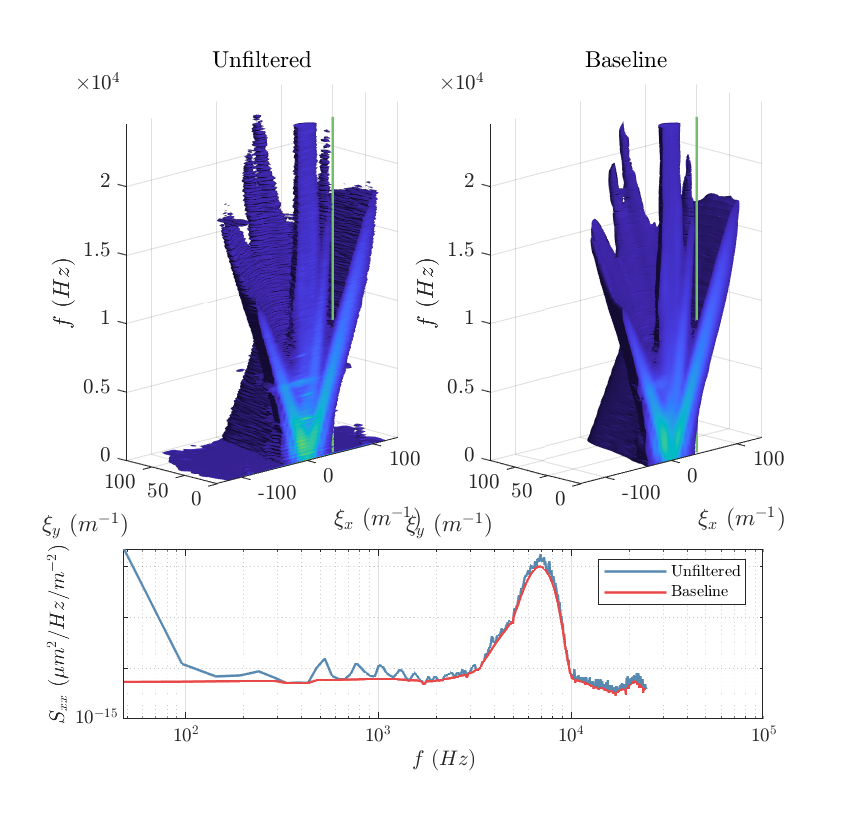
\includegraphics{../matlab/06_single_sensor_filtering/filter_baseline.eps}
  \caption{Baseline spectrum estimation. The top left plot shows the unfiltered multidimensional spectrum and the baseline spectrum on the top right. The green line in each of these plots represents the location at which the spectra in the bottom plot is shown.}
  \label{fig:06_filter_baseline}
\end{figure}
The bottom plot of the figure shows the unfiltered and baseline spectra along the green line in the two multidimensional spectral plots.
The total power of the signal has been reduced by $~71\%$ with all of the narrow-band signals removed.
A large portion of this signal removal is the very low temporal frequency components.
The blade-passing frequency and harmonics are completely removed but the broadband acoustic duct-modes remain intact.
The peak of the boundary-layer signal is reduced slightly as well as the high frequency fluctuations.

\section{Basic Filter Summary}
Three different basic wavefront filters were shown and discussed in this chapter.
The temporal filter is most useful when filtering out a frequency band of optical noise.
Besides filtering out optical noise, band-pass filters can be used to analyze a wavefront over a narrow-band to examine the optical aberrations at specific frequencies that significantly contribute to the overall optical disturbance; for example, as was shown in Chapter \ref{chap:03_optical_acoustics}, band-pass filters along with an implementation of an acoustic mode-marching method can help determine with some confidence that a narrow-band signal is likely to have been created by the wind-tunnel fan and can be removed.

Filters that separate upstream and downstream-moving disturbances are useful to filter out the optical contamination that comes from acoustic signals that are traveling upstream from a wind-tunnel fan.
These filters would also be useful for separating out an aero-optical signal that has a broad range of velocities that can occur in a span wise measurement of a boundary layer.
The velocity filter is the most useful for isolating the aero-optical portion of a wavefront measurement given the aero-optical signal has a fairly narrow and constant velocity range.
This filter also can be used to measure the speed associated with an optical disturbance in both x and y-directions.

The spectral baseline provides a simple way of removing all of the narrow-band signals with slight attenuation to the broadband signals.
The broadband acoustic and stationary modes remain but could be filtered with via other techniques such as using a velocity filter.
Narrow-band features that are not likely to be environmental contamination could be easily added back in.

\section{Multiple Sensor Filtering of Optical Wavefronts}
In the previous sections, methods of filtering optical wavefront corruption by applying a variety of filters to the wavefront in the multidimensional spectral domain were investigated.
These techniques involve only data from the optical wavefront itself and user knowledge and experience to obtain filtered data.
When additional data are available, such as from microphones or accelerometers, a targeted filter approach becomes possible.

This kind of approach is described in a previous study \cite{DeLucca-2014-RAJvGdv7} in which a combination of linear stochastic estimation (LSE) and spectral proper orthogonal decomposition (SPOD) was used to remove vibration related contamination from aero-optical wind-tunnel measurements.
This process along with optical tip and tilt removal showed approximately an 85\% removal of contamination in the measured $\opdrms$ by using accelerometer measurements to remove vibration effects from optical wavefront measurements.

Finally, this chapter concludes by showing results produced by applying the LSE-SPOD filter to experimental wavefront data acquired in the White Field wind tunnel, both by itself and in combination with the filters described in Chapter \ref{chap:06_single_filter}. The objective of the filtering approaches shown was to filter out contamination from the aero-optical signal produced by the boundary layer on the measurement aperture. The performance of the various filtering methods are compared and recommendations for the best filtering approach are given.

\subsection{Optical Tip and Tilt}
Although they are usually not employed in aero-optical investigations, Zernike polynomials have been traditionally used for modal decomposition of the optical aberrations of an optical system \cite{Born-1965-HHGYgjdH}.
These polynomials are defined on the unit circle and form a set of orthogonal functions,
\begin{equation}
  Z_n^m(\rho,\theta) = R_n^m(\rho)\cos(m\theta)
  \label{eqn:07_zernike}
\end{equation}
where $R_n^m(\rho)$ is the radial basis function and $\cos(m\theta)$ is the angular basis function.
For values of $-m$ the angular basis function becomes $\sin(m\theta)$.
The radial basis functions are developed from Jacobi polynomials but for purposes of this study, only a few simple ones will be used.
An optical wavefront can be represented by a summation of Zernike polynomials multiplied by their corresponding coefficients
\begin{equation}
  \wf = \sum Z_ja_j \textrm{.}
  \label{eqn:07_zernike_coeff}
\end{equation}

The Noll naming scheme is a method of organizing the Zernike polynomials into a single notation of $Z_j$, along with normalizing each polynomial to have a spatial RMS equal to one \cite{Noll-1976-HHKzd88f}.
The first three of these using the Noll naming scheme are piston, tip, and tilt.
Piston is simply the average $\opd$ value of the wavefront
\begin{equation}
  Z_1 = 1 \textrm{.}
  \label{eqn:07_zernike_1}
\end{equation}
Tip and tilt are the best planar fit to the $\opd$ along the x-axis and y-axis respectively where tip is
\begin{equation}
  Z_2 = 2\rho\cos\theta \textrm{,}
  \label{eqn:07_zernike_2}
\end{equation}
and tilt is
\begin{equation}
  Z_3 = 2\rho\sin\theta \textrm{.}
  \label{eqn:07_zernike_3}
\end{equation}
Once the coefficients for these modes are solved for they can be removed from the original wavefront, $WF$:
\begin{equation}
  WF^F = WF-\sum Z_ja_j \textrm{.}
\end{equation}

\subsection{LSE-SPOD}
The LSE-SPOD technique starts with performing SPOD on the primary data set and then using the Fourier transforms of the additional sensor data to perform a filtering operation.
The spectral proper orthogonal decomposition technique is described in detail by Schmidt and Colonius \cite{Schmidt-2020-m2emACkX}.
A schematic of the SPOD algorithm is shown in Figure \ref{fig:07_spod_algorithm}.
\begin{figure}
  \centering
  \includegraphics{../other-sources/schmidt_2020_figure_01.jpeg}
  \put(-20,235){\fcolorbox{white}{white}{\footnotesize(\ref{eqn:07_data_block})}}
  \put(-230,210){\rotatebox{90}{\fcolorbox{white}{white}{\color{white}{empt}}}}
  \put(-20,102){\fcolorbox{white}{white}{\footnotesize(\ref{eqn:07_frequency_block})}}
  \put(-231,69){\rotatebox{90}{\fcolorbox{white}{white}{\footnotesize(\ref{eqn:07_pod_01}-\ref{eqn:07_pod_04})}}}
  \caption{Schematic of the SPOD algorithm (taken from \cite{Schmidt-2020-m2emACkX}). The numbers in parentheses denote the equations used.}
  \label{fig:07_spod_algorithm}
\end{figure}
The algorithm begins by separating the original data set, $Q$, into a number of smaller blocks,
\begin{equation}
  Q = \left[
  \begin{matrix}
    \mid & \mid & & \mid \\
    q^{(1)} & q^{(2)} & \cdots & q^{(N)} \\
    \mid & \mid & & \mid
  \end{matrix}
  \right]\textrm{,}\quad Q\in\mathbb{C}^{M\times N}
  \label{eqn:07_data_block}
\end{equation}
where $M$ is the total number of degrees of freedom (number of spatial points times the block length in time) and $N$ is the number of blocks.
Each block is then Fourier Transformed in the temporal dimension or through all dimensions.
Once in the frequency domain the data blocks are then reorganized by creating new blocks of identical temporal-frequencies,
\begin{equation}
  \hat{Q} = \left[
  \begin{matrix}
    \mid & \mid & & \mid \\
    \hat{q}^{(1)} & \hat{q}^{(2)} & \cdots & \hat{q}^{(N)} \\
    \mid & \mid & & \mid
  \end{matrix}
  \right]\textrm{,}\quad \hat{Q}\in\mathbb{C}^{M\times N}
  \label{eqn:07_frequency_block}
\end{equation}
where $M$ is now the number of spatial points times the number of blocks and $N$ is block length in time.
Proper orthogonal decomposition is then performed separately on each temporal-frequency block via either traditional POD
\begin{equation}
  \hat{C} = \frac{1}{N-1}\hat{Q}\hat{Q}^H \textrm{,}
  \label{eqn:07_pod_01}
\end{equation}
\begin{equation}
  \hat{C}W\hat{\Phi}=\hat{\Phi}\hat{\Lambda} \textrm{,}
  \label{eqn:07_pod_02}
\end{equation}
or the method of snapshots,
\begin{equation}
  \hat{Q}^HW\hat{Q}\hat{\Psi}=\hat{\Psi}\hat{\Lambda} \textrm{,}
  \label{eqn:07_pod_03}
\end{equation}
\begin{equation}
  \hat{\Phi}=\hat{Q}\hat{\Psi} \textrm{,}
  \label{eqn:07_pod_04}
\end{equation}
where $H$ denotes the Hermitian transpose, $W$ is a weighting matrix, $\Phi$ is the set of deterministic spatial functions, $\Lambda$ is the eigen-values, and $\Psi$ is the coefficient matrix.

The linear stochastic estimation portion of the technique is described by Adrian \cite{Adrian-1975-VenaZyuv}.
This process uses a linear sum, $L_{ij}$, of additional measurements, $y_j$, to approximate a measured signal, $x_i$,
\begin{equation}
  x_i^{LSE}=L_{ij}y_j \textrm{,}
  \label{eqn:07_lse_01}
\end{equation}
where
\begin{equation}
  L_{ij} = \langle x_iy_k\rangle\langle y_jy_k\rangle^{-1} \textrm{.}
  \label{eqn:07_lse_02}
\end{equation}
When combined with SPOD, the estimation matrix, $L$, becomes
\begin{equation}
  L=(\hat{\Psi}\hat{y}^H)(\hat{y}\hat{y}^H)^{-1} \textrm{,}
  \label{eqn:07_lse_spod_01}
\end{equation}
which allows for an estimated version of the coefficient matrix to be calculated
\begin{equation}
  \hat{\Psi}^E=L\hat{y} \textrm{.}
  \label{eqn:07_lse_spod_02}
\end{equation}
The estimated coefficient matrix contains portions of the original signal that best resemble the additional sensor data.
Assuming that the additional sensor data represents signal contamination of the original signal, a filtered coefficient matrix can be computed from the difference between the original and estimated coefficient matrices.
\begin{equation}
  \hat{\Psi}^F=\hat{\Psi}-\hat{\Psi}^E \textrm{.}
  \label{eqn:07_lse_spod_03}
\end{equation}
A filtered signal, $Q^F$ can be constructed by using the filtered coefficient matrix and the spatial functions,
\begin{equation}
  \hat{Q} = \hat{\Psi}^F\hat{\Phi}^H \textrm{.}
\end{equation}

\subsection{Filtering Experimental Data}
The filtering technique described in the preceding section was applied to the same data sets that were shown in Figure \ref{fig:04_dispersion_mach}, either separately or in combination with the basic filtering methods described earlier in this chapter.
Simultaneous accelerometer and microphone measurements were made alongside the optical wavefront measurements.
The locations of some of the additional sensors are shown in Figure \ref{fig:07_sensor placement} with a CAD drawing of the test section in Figure \ref{fig:07_test_section_mic_accel}.
Table \ref{tab:07_sensor_list} shows a list of the additional sensors including the number designation used in Figures \ref{fig:07_sensor placement} and \ref{fig:07_test_section_mic_accel}, the model of the sensor and preamplifier used as well as a sensor grouping designation.
\begin{figure}
  \centering
  \includegraphics[trim={0 0 5in 3in},clip,width=0.9\textwidth]{../photos/IMG_9655.jpeg}
  \put(-65,120){\circledfill{\large 1}}
  \put(-40,220){\circledfill{\large 3}}
  \put(-50,165){\circledfill{\large 4}}
  \put(-125,40){\circledfill{\large 7}}
  \put(-243,240){\circledfill{\large 8}}
  \put(-180,120){\circledfill{\large 9}}
  \put(-320,110){\circledfill{\large 10}}
  \caption{The locations of some of the additional sensors used in the LSE-SPOD filtering. The sensors are labeled with the sensor numbers, see Table \ref{tab:07_sensor_list}.}
  \label{fig:07_sensor placement}
\end{figure}
\begin{figure}
  \centering
  \includegraphics[trim={1in 2.75in 1in 2.75in},clip,width=0.9\textwidth]{../cad/test_section_mic_accel.pdf}
  \put(-272,77){\circled{\large 3}}
  \put(-274,60){\circled{\large 4}}
  \put(-131,61){\circled{\large 5}}
  \put(-133,45){\circled{\large 6}}
  \put(-203,82){\circled{\large 8}}
  \put(-220,46){\circled{\large 9}}
  \put(-188,46){\circled{\large 10}}
  \put(-188,12){\squared{\large 11}}
  \put(-243,100){\squared{\large 12}}
  \put(-140,100){\squared{\large 13}}
  \put(-350,10){\Large Flow $\Longrightarrow$}
  \caption{CAD drawing view of the inside of the test-section with some of the sensor locations labeled. Flow is from left to right. The numbers in the circles are the sensor numbers on the model side of the test-section. The numbers in the square are the sensor numbers opposite of the model side. The dashed line represents the optics window opposite of the model for the beam angle of $90^\circ$. The window was moved up and downstream depending on the beam angle.}
  \label{fig:07_test_section_mic_accel}
\end{figure}
\begin{table}
  \centering
  \caption{Additional sensors used the the LSE-SPOD filtering.}
  \begin{tabular}{c c c c c}
    Channel & Sensor Type & Model & Preamp & Group\\
    \hline \hline
    1 & Microphone & ACO 7016B & B\&K 2690 & Ambient \\
    2 & Microphone & B\&K 4939 & B\&K 2690 & Ambient \\
    3 & Microphone & PCB 103B02 & PCB 483C & Test Section \\
    4 & Microphone & PCB 103B02 & PCB 483C & Test Section \\
    5 & Microphone & PCB 103B02 & PCB 483C & Test Section \\
    6 & Microphone & PCB 103B02 & PCB 483C & Test Section \\
    7 & Accelerometer & PCB 352C33 & PCB 483C & Primary Lens \\
    8 & Accelerometer & PCB 352C33 & PCB 483C & Test Section \\
    9 & Accelerometer & PCB 352C33 & PCB 483C & Test Section \\
    10 & Accelerometer & PCB 352C33 & PCB 483C & Test Section \\
    11 & Accelerometer & PCB 352C33 & PCB 482A22 & Test Section \\
    12 & Accelerometer & PCB 352C33 & PCB 482A22 & Test Section \\
    13 & Accelerometer & PCB 352C33 & PCB 482A22 & Test Section \\
    14 & Accelerometer & PCB 352C33 & PCB 482A22 & Optics Bench \\
    15 & Accelerometer & PCB 352C33 & PCB 482A22 & Return Mirror \\
    16 & Accelerometer & PCB 352C33 & PCB 482A22 & Return Mirror \\
  \end{tabular}
  \label{tab:07_sensor_list}
\end{table}
All of the test-section mounted sensors are shown in their approximate locations in Figure \ref{fig:07_test_section_mic_accel} in a view that is looking at the wind-tunnel model from inside of the test-section with the flow moving from left-to-right.
The dashed box represent the optical window on the opposite side of the tunnel from the model which was moved up or downstream depending on the beam angle relative to the flow.
Sensors 11-13 were attached to this optical window and moved with it.
The picture in Figure \ref{fig:07_sensor placement} was taken from the opposite side of the test-section and model that is shown in Figure \ref{fig:07_test_section_mic_accel} and as such the flow goes from right-to-left.

Two microphones were used for ambient measurement (a ACO 7016B \cite{ACO-Microphones} and a Br\"uel \& Kj\ae r 4939 \cite{Bruel-Kjaer-4939}), four microphones were used for test-section noise measurement (PCB 103B02 \cite{PCB-103B02-C}), and ten accelerometers were located throughout the setup (PCB 352C33 \cite{PCB-352C33-H}).
One of the ambient microphones was mounted to the top of the optics bench facing the test-section and can be seen in Figure \ref{fig:07_sensor placement} just to the right of the primary lens and the other ambient microphone was hanging below the optics bench end towards the test-section.

The test-section microphones were in groups of two either upstream or downstream from the optical beam by about 20-inches, with the upstream microphone locations viewable in Figure \ref{fig:07_sensor placement} (sensors 3 and 4) and shown in Figure \ref{fig:07_test_section_mic_accel}.
The model installed in the test-section represents the outside of an aircraft fuselage with a 5-foot diameter and is angled to account for the aircraft's angle-of-attack (~6$^\circ$) for steady-level-flight at cruise.
This results in the fuselage model being shifted approximately 2-inches higher from the test-section centerline upsteam at the microphone location.
The duct microphones were placed about 2.75-inches from the model centerline.

There were six accelerometers attached to the test-section windows, with three being on each side as shown in Figure \ref{fig:07_test_section_mic_accel}.
The locations of the three accelerometers (sensors 8-10) on the model side can be seen in Figure \ref{fig:07_sensor placement}, the three accelerometers on the other window used the opposite pattern (two high and one low).
The optical window on the far side of the test-section was moved laterally depending on the angle of the beam relative to the flow.
One accelerometer was placed on the primary lens (also shown, sensor 7) and one was placed in the center of the optics bench.
The last two accelerometers were located on the back of the return mirror with one on the top and the other on the side.

\section{Results}
The power-spectra of all of the sensors at the three Mach numbers are shown in Figure \ref{fig:07_sensor_spectra}.
\begin{figure}
  \centering
  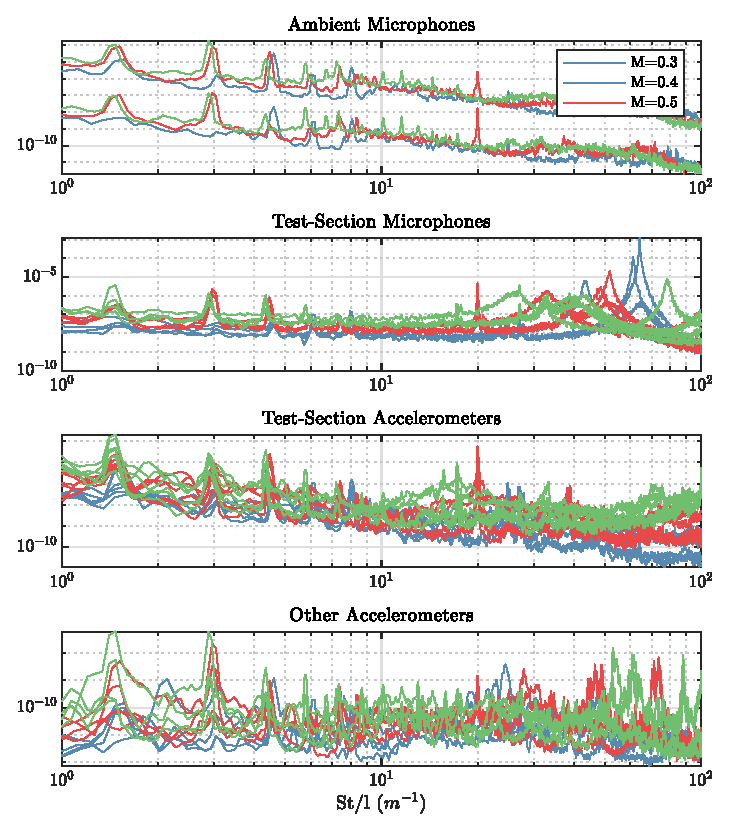
\includegraphics{../matlab/07_multiple_sensor_filtering/sensor_spectra.eps}
  \caption{Power-spectra of the additional sensor measurements at the three Mach numbers tested. The x-axis is in Strouhal number per characteristic length ($St/l$).}
  \label{fig:07_sensor_spectra}
\end{figure}
These plots are presented as Strouhal number per unit characteristic length, since this puts the signals related to the fan blade-passing frequency at the same x-axis location for all three tested wind speeds.
Figure \ref{fig:07_sensor_spectra} also shows the different groups of sensors shown together in separate plots.
The blade-passing frequency for these data sets is at a $St/l$ of approximately 3 $m^{-1}$ with a clear and consistent narrow-band signal at that $St/l$ for all but the $M=0.3$ run, which has a slight increase in signal for some of the sensors.
For the $M=0.5$ case there is an additional strong narrow-band signal at 20 $m^{-1}$ for all sensors and a slightly broader signal at 38 $m^{-1}$ that is only present in the test-section mounted sensors that may be due to extra fan vibration which was limiting the top speed of the wind-tunnel.
The test-section mounted microphones are picking up boundary layer acoustic noise above $St/l$ of approximately 20 $m^{-1}$.

Two variants of the filtering technique were tried.
The first was a standard LSE-SPOD technique in which the spectral POD was performed on the data set that was Fourier transformed in time only.
For the second technique, which will be referred to here as LSE-MSPOD, the spectral POD was applied to a data set in which the Fourier transform was performed in all dimensions of space and time, which is a portion of the computation for the multidimensional spectral estimation.
Figures \ref{fig:07_lse_spod} and \ref{fig:07_lse_mspod} show multidimensional power spectrum plots at a temporal block length of $2^{10}$ with no overlap.
\begin{figure}
  \centering
  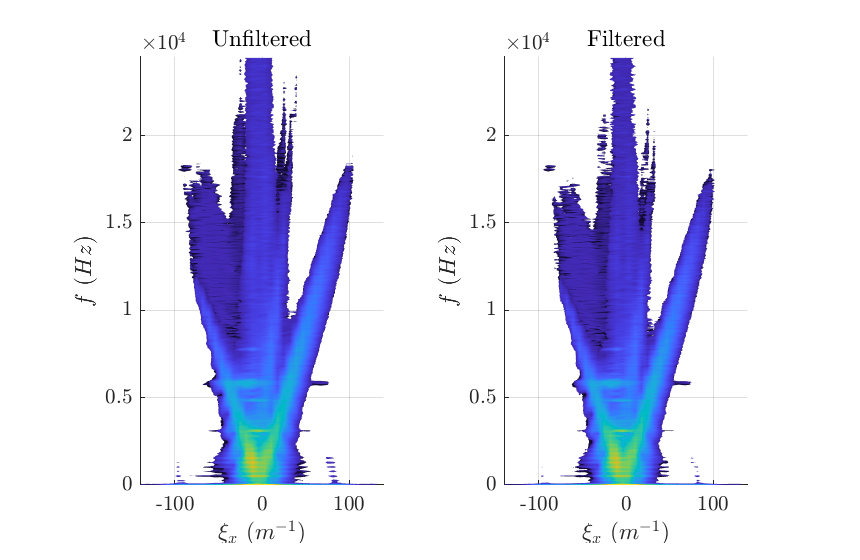
\includegraphics{../matlab/07_multiple_sensor_filtering/lse_spod.eps}
  \caption{A multidimensional power spectrum of an unfiltered wavefront and the same wavefront filtered with the LSE-SPOD method using all 16 additional microphone or accelerometer measurements.  }
  \label{fig:07_lse_spod}
\end{figure}
\begin{figure}
  \centering
  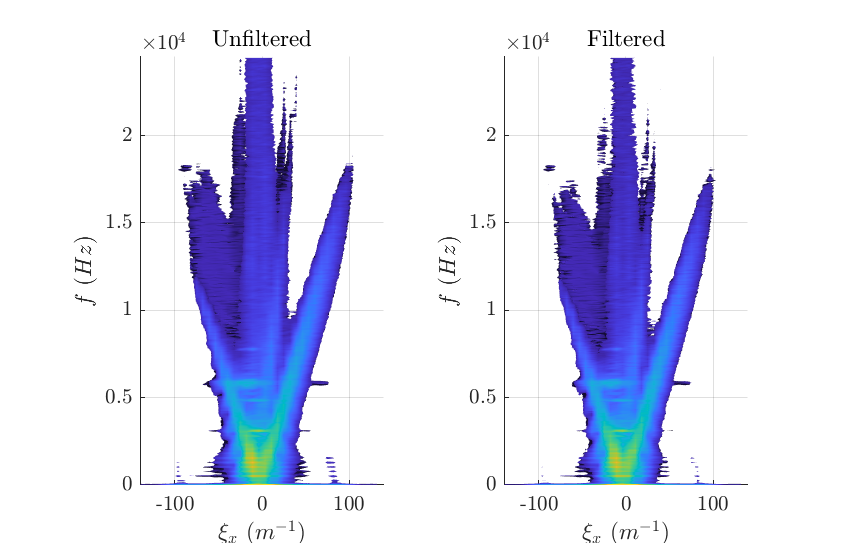
\includegraphics{../matlab/07_multiple_sensor_filtering/lse_mspod.eps}
  \caption{A multidimensional power spectrum of an unfiltered wavefront and the same wavefront filtered with the LSE-MSPOD method using all 16 additional microphone or accelerometer measurements.  }
  \label{fig:07_lse_mspod}
\end{figure}
These plots show the $f$-$\xi_x$ plane of the multidimensional spectrum that captures horizontally-moving (streamwise) plane waves with a portion of the acoustic cone isosurface wrapping behind it.
Both of these methods performed effectively identically to one another with a 14.2\% drop in overall RMS value of the filtered wavefront (both time and space).
There is a significant drop in the signal at the blade-passing frequency and its harmonics, especially at the higher spatial frequencies.
The stationary signal information is also significantly reduced along with the high temporal-frequency acoustic signal.
The aero-optical boundary layer signal is also partially reduced, which is most noticeable at higher temporal-frequencies.
% Some of this lost signal can be restored by increasing the overlap of the temporal frequency blocks, but this also restores some of the unwanted high temporal-frequency contamination.

\begin{table}
  \centering
  \caption{$\opdrms$ ($\mu m$) comparison of using different combinations of additional sensor information in the LSE-MSPOD filtering process.}
  \input{../matlab/07_multiple_sensor_filtering/lse_mspod_table.txt}
  \label{tab:07_lse_mspod_table}
\end{table}

Table \ref{tab:07_lse_mspod_table} shows the time averaged $\opdrms$ of three different data sets at a beam angle through the test-section of $90^\circ$.
The data sets were at Mach numbers of 0.3, 0.4, and 0.5 and had an unfiltered $\opdrms$ of 0.0561, 0.0521, and 0.0824 $\mu m$ respectively.
Note that in the raw processed wavefronts, the $\opdrms$ at a Mach number of 0.3 was higher than the 0.4 case.
There was a significant drop of between 62.6\% and 78.6\% in the $\opdrms$ by removing the Zernike modes corresponding to tip and tilt.
It is at this point the Mach number of 0.4 case has a higher $\opdrms$ than the 0.3 case as would be expected \cite{Gordeyev-2014-jcJndkHM}.
Note that it is standard practice to remove optical tip/tilt from wavefront measurements, since tip/tilt is largely imposed by the measurement optics rather than the actual aero-optical flow.

Table \ref{tab:07_lse_mspod_table} also shows the effect of five different combinations of additional sensors that were used for filtering with the LSE-MSPOD process (the bracketed percentage in Table \ref{tab:07_lse_mspod_table} shows the percent reduction in $\opdrms$ due to the filtering).
The first set was all of the accelerometers which resulted in an additional drop in $\opdrms$ of between 3\% and 5\%.
The second and third sets used either the ambient or duct microphones and those sets had slightly less reduction than the accelerometers.
The fourth set was the test-section sensors comprised of six window mounted accelerometers and four duct mounted microphones.
This set of sensors performed the same as all of the accelerometers, while the use of all of the additional sensors in the last set performed the best, with an additional reduction in $\opdrms$ of 4 to 6\% from the tip/tilt removal cases.

% A velocity filter was also tried in addition to just the tip/tilt removal or in conjunction with tip/tilt and all the sensors being used in the LSE-MSPOD process.
% The velocity filter performed better than the all-sensors removal case by an additional 1.5 to 3\% but some of the narrow-band signals remain.
% When all sensors were used with LSE-MSPOD on the velocity filtered wavefronts an additional 3 to 4\% of the $\opdrms$ was removed compared to just the velocity-filtered case or an additional 8.1\% reduction for only doing tip/tilt removal on the Mach number of 0.3 case or 14.1 and 13.3\% reduction for the 0.4 and 0.5 Mach number cases.

In summary, Table \ref{tab:07_lse_mspod_table} shows that using either the temporal or multidimensional version of the LSE-SPOD filtering technique can help remove some of the narrow-band acoustic and vibration reduction in an optical wavefront.
These temporally narrow-band signals have broadband spatial content that is attenuated.
This additional reduction does seem to be somewhat tied to the number of sensors used with more sensors having a greater impact on the signal reduction.
Since the vibrations and acoustics have the same primary source, the wind-tunnel fan, they seems to do a relatively equivalent job at filtering the optical contamination.
Accelerometers have the benefit of easier installation but the microphones do not necessarily have to be installed inside of the wind-tunnel.

    % !TEX root = catron-dissertation.tex
\epstopdfsetup{outdir=./images/07_multiple_sensor_filtering/}

\chapter{Multiple Sensor Filtering Techniques}
\label{chap:07_multiple_filter}

    % !TEX root = catron-dissertation.tex
\epstopdfsetup{outdir=./images/08_conclusion/}

\chapter{Conclusion}
\label{chap:08_conclusion}

When aero-optical measurements are made in a wind tunnel, there are a number of sources that contaminate the measurement with noise.
This can be seen in Figure \ref{fig:08_dispersion_isosurface} which shows a multidimensional spectral estimation of an optical wavefront measurement made in a wind tunnel.
\begin{figure}
  \centering
  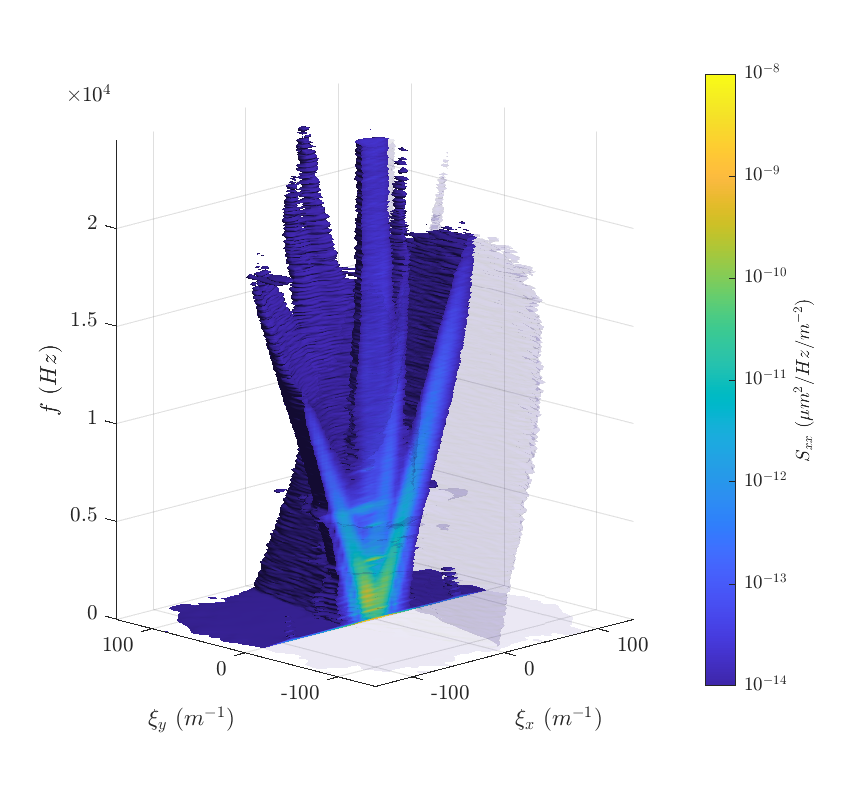
\includegraphics{../matlab/08_conclusion/dispersion_isosurface.eps}
  \put(-195,120){\rotatebox{76}{\Large Boundary Layer}}
  \put(-305,250){\rotatebox{-75}{\Large Acoustic Cone}}
  \put(-300,69){\textcolor{white}{\Large BPF $\Longrightarrow$}}
  \put(-231,180){\textcolor{white}{\rotatebox{90}{\Large Stationary Modes}}}
  \put(-235,50){\rotatebox{15}{\Large Mean-Lensing}}
  \caption{Multidimensional spectral estimation of an optical wavefront measurement made in a wind tunnel.}
  \label{fig:08_dispersion_isosurface}
\end{figure}
Figure \ref{fig:08_dispersion_isosurface} shows the full multi-dimensional spectrum for wavefront data acquired in a wind tunnel, including streamwise and vertical spatial frequencies ($\xi_x$ and $\xi_y$), and temporal frequencies ($f$); however, in
in Figure \ref{fig:08_dispersion_isosurface}, the half of the isosurface which represents the portion of the signal that has a component that is traveling vertically downward has been made transparent to show some of the internal auto-spectral density of planar waves that are traveling parallel to the direction of flow.

In Figure \ref{fig:08_dispersion_isosurface}, the aero-optical signal that is considered to be the objective of the measurement is the boundary layer which resembles a thin ellipsoid that has an angle in the $x-\xi_x$ plane (where the $xi_x$-coordinate represents spatial frequencies in the stream-wise direction) by an amount related to the free-stream velocity (see Equation \ref{eqn:04_velocity_assumed}).
Acoustic duct modes make up a temporally broadband signal that forms a cone and have a significant portion of the signal that travels upstream.
In the $\xi_x-f$ plane the outer surface of the acoustic cone is limited by the sonic lines at $u\pm c$, while in the $\xi_y-f$ plane the limit is at $\pm c$.
The wind-tunnel fan produces temporally narrow-band acoustic and vibration modes that are able to contaminate the wavefront measurement at the blade-passing frequency (BPF) and its various harmonics.

Sources of noise shown in Figure \ref{fig:08_dispersion_isosurface} not related to the acoustics include stationary modes and mean-lensing.
The stationary modes do not travel in any direction, their spatial frequencies are near zero and their signal strength is fairly constant in time.
Due to the temporally white-noise nature of this signal, it is likely not physically relevant and could be optical mode noise from the laser, electronic noise in the camera, or even numerical noise from the processing code.
At lower frequencies, especially around the blade-passing frequency or its harmonics, there is likely a significant number of stationary modes that are due to vibration of various optical elements.
The mean-lensing portion of the signal ($\lessapprox 100$ Hz) is a slowly varying signal with large spatial frequency content.
A color coded multidimensional spectral estimation plot that allows for easier identification of the various component signals is shown in Figure \ref{fig:05_synthetic_dispersion_input} and was used for generating a synthetic wavefront.
As such, a major contribution of this dissertation research is an improved understanding of the signals and contamination that appear in aero-optical data, and how those signals appear in multi-dimensional spectra. This information provides a better understanding of aero-optical data, as well as guidance towards methods of filtering out contaminating noise sources.

\section{Filtering of Optical Wavefronts}
Two main families of filtering techniques were examined in this dissertation.
The first family was single sensor filters, Chapter \ref{chap:06_single_filter}, which operate on the optical wavefronts without knowledge of any other time resolved data.
Some of these filters may rely on additional information about the average sampling conditions used to measure the wavefronts.
The second family was multiple sensor filters, Chapter \ref{chap:07_multiple_filter}, which filter the optical wavefront using time resolved measurements from additional sensors.

\subsection{Single Sensor Filters}
The single sensors filters operated directly on the optical wavefront measurements.
Most of these filters are based on Butterworth filters \cite{Butterworth-1930-DvDrjKha} that operate in the multidimensional Fourier domain using a transfer function, $\hat{H}(\xi_x,\xi_y,f)$,
\begin{equation}
  \widehat{WF}(\xi_x,\xi_y,f) = \hat{H}(\xi_x,\xi_y,f)\fftthree(wf(x,y,t)) \textrm{,}
\end{equation}
which can be inverse Fourier transformed back into the physical domain or be used for calculating the multidimensional spectrum.
Filtering can also be performed on the multidimensional spectrum using the gain function, $G^2 = \hat{H}\hat{H}^*$,
\begin{equation}
  S_{xx}(\xi_x,\xi_y,f) = G^2(\xi_x,\xi_y,f)S_{xx}(\xi_x,\xi_y,f) \textrm{.}
\end{equation}
The only filter that was investigated that was not based on basic filters was a baseline spectrum estimator \cite{Schulze-2012-GmyAqzC7}.
This filter removes narrow-band peaks and noise peaks along the temporal frequency axis smooth spectrum.

\section{Other Useful Products}

\subsection{Synthetic Wavefront}
A synthetic wavefront was developed in Chapter \ref{chap:05_synthetic} to test various filters used in Chapter \ref{chap:06_single_filter}.
In the process used to create the synthetic wavefront, each of these signal components was generated separately in the multidimensional spectrum.
While this synthetic wavefront generation technique produced a qualitative approximation of a wavefront, it provided a useful set of fully known data to test various filters.
There is some significant room for improvement in the process of creating synthetic wavefronts that are more physically accurate.
Even without improvement this process may be useful in generating a set of synthetic wavefronts with a known aero-optical and noise components that can be used for training a neural network to filter \cite{Lo-1994-W6aWeuaT} wavefront measurements.
A neural network based filter may be able to separate the overlapping component signals at low frequencies.

\subsection{Measuring Acoustic Field Optically}
In section \ref{sect:03_examples_spherical}, optical wavefront were shown to have a fairly good agreement with a microphone for measuring the fluctuating field strength of a spherical wave generated by a speaker.
The optical wavefront measurement however had issues when the acoustic field diverged from being nearly spherical.
Optical wavefronts can be a method to non-intrusively measure an acoustic field, although the beam-path integrated results of the wavefront measurement require additional interpretation to extract information on the acoustic field.

\subsection{Acoustic Mode-Marching}
An acoustic mode-marching method was developed to quickly estimate the acoustic field within a wind-tunnel test-section assuming that the primary noise source was the wind-tunnel fan.
Although, this is likely to have limited application in filtering of optical wavefronts, it is useful for assisting researchers in determining whether specific narrow-band signals are produced by the wind-tunnel fan and can be filtered out.
Since there may be upstream-traveling components of the aero-optical signal such as that produced by recirculation zones or sound produced by the test model, the capability to definitively identify the optical signal produced by the wind-tunnel main fan is useful information.
There also maybe some application during the initial design of a tunnel for estimating the acoustic field in some critical components.

\section{Recommendations For Future Research}

Future research is needed to better validate these filtering techniques as well as aid in the development of future filtering techniques.
This in part can be accomplished by making a series of measurements on different models that differ only in scale.
For turrets the aero-optical signal can be normalized \cite{Jumper-2013-8KtN3pue},
\begin{equation}
  \opd_{NORM} = \frac{\opd}{\left(\frac{\rho_0}{\rho_{SL}}\right)M^2D} \textrm{,}
\end{equation}
where $\rho_0$ is the free-stream total density of the flow around the turret, $\rho_{SL}$ is the density of air at sea-level, and $D$ is the turret diameter.
This equation allow the aero-optical signal to be scaled to different models.
Test results from different scale models should be in agreement after the signal contamination is removed.

A detailed set of measurements should be produced capturing not only the aero-optical mesurements but also simultaneous sound and vibration measurements.
This has been partially done before with hemispherical and hemisphere-on-cylinder turrets, but other geometries such as partial-hemisphere or generic-pod-based geometries need a test database as well.
Optical wave-front measurements behind a turbulent wake from a cylinder may even prove to be useful.

There is a lot of research that can still be done on various filtering techniques to remove signal contamination of aero-optical wavefront measurements.
This is especially true for filters that can utilize additional sensor measurements.
The process for creating the synthetic wavefronts used in this research was a qualitative approximation that can be made more physically accurate.
Synthetic signal algorithms could be developed for types other aero-optical disturbances such as sheer layers \cite{Jumper-2017-8UnkaeqW}.
Synthetic wavefront signals could aid in the testing of algorithms used on adaptive optic systems.
The acoustic mode-marching analysis could be expanded to the case where a simple model in the wind-tunnel test section.


  % \appendix
  %   % !TEX root = catron-dissertation.tex
\chapter{Sample Code}

\lstinputlisting[label=code:sc_simpleSXX, caption={A simple function for computing the power spectra for vector \lstinline{x} given an arbitrary windowing function.}, language=Matlab]{../matlab/00_functions/simpleSXX.m}

\lstinputlisting[label=code:sc_simpleSXXn, caption={A simple function for computing the dispersion or n-dimensional power spectra of \lstinline{x} given an arbitrary windowing function.}, language=Matlab]{../matlab/00_functions/simpleSXXn.m}

\lstinputlisting[label=code:sc_synthetic_wavefront, caption={MATLAB code used to generate the synthetic wavefront used in Chapter \ref{chap:wavefront_filtering}.}, language=Matlab]{../matlab/05_synthetic_wavefront/synthetic_wavefront.m}

\lstinputlisting[label=code:sc_basic_wavefront_filters, caption={MATLAB code used to filter wavefronts in Chapter \ref{chap:wavefront_filtering}.}, language=Matlab]{../matlab/00_functions/WFfilter.m}

% \lstinputlisting[label=code:sc_spatial_window, caption={MATLAB code used to generate a spatial windowing function for an arbitrary two-dimensional mask.}, language=Matlab]{../matlab/00_functions/createSpatialWindow.m}

% \lstinputlisting[label=code:wfdispersion, caption={Dispersion analysis code}, language=Matlab]{../matlab/00_functions/WFdispersion.m}

    % % !TEX root = catron-dissertation.tex

\chapter{N-Dimensional Power Spectral Density}
\label{chap:ap_nd_psd}

This appendix will go through the process of obtaining a n-dimensional form of the power spectral density formula.
For a point in physical space or time, the variable $x$ will be used, while frequency space will use the variable $\xi$.


\section{1-Dimensional Continuous}
\begin{equation}
  F(\xi) = \int_{-\infty}^{+\infty} f(x)\exp\{-2\pi j x \xi\} dx
\end{equation}
\cite{Kammler-2007-ypxvyGCJ}


\begin{equation}
  S_{xx}(\xi) = \lim_{X \to \infty}\frac{1}{X}|F(\xi)|^2
\end{equation}
\cite{Miller-2012-2E7ckWtR}

\section{1-Dimensional Discrete}
\begin{equation}
  F[\xi] = \frac{1}{N}\sum_{n=0}^{N-1}f[n]\exp\{-2\pi jn\xi/N\}
\end{equation}
\cite{Kammler-2007-ypxvyGCJ}

\begin{equation}
  S_{xx}[\xi] = \frac{1}{N}   |F[\xi]|^2
\end{equation}


\section{1-Dimensional Comparison}


\section{N-Dimensional Continuous}
\begin{equation}
  F(\mathbf{\xi}) = 
\end{equation}


  \backmatter
    \bibliographystyle{nddiss2e}
    \bibliography{99_references.bib}
\end{document}
